In this section we study the performance of various groomed jet
masses, substructure variables, and BDT combinations of groomed mass
and substructure, in terms of the
identification of a boosted hadronically decaying $W$ signal aginst a gluon-gluon
background. We produce Receiver Operating Characteristic (ROC)
curves that elucidate the performance of the various groomed mass and
substructure variables that are
capable of providing discrimination between signal and background. A
range of different distance parameter settings for the \antikt~jet
algorithm are explored, in a variety of kinematic regimes
(lead jet \pt 200-300 GeV, 500-600 GeV, 1.0-1.1 TeV), to explore the
performance as a function of jet radius and jet boost, and to see
where substructure approaches may break down. The groomed
mass and substructure variables are then combined in a Boosted Decision Tree (BDT), and the performance of the resulting BDT discriminant
explored through ROC curves to understand the degree to which
variables are correlated and exploiting the same information, and how
this changes with jet boost and jet radius. 

\subsection{Methodology}

These studies use the $X \rightarrow WW$ samples as signal and the $gg$
samples to model the QCD background, described previously in Section~\ref{sec:samples}. Whilst only gluonic backgrounds
are explored here, the conclusions as to the dependence of the
performance and correlations on the jet boost and radius have been
verified to hold also for $qq$ backgrounds. {\it To be checked!}

Jets are reconstructed using the \antikt algorithm, and have various
jet grooming approaches applied, as described in Section~\ref{sec:jetalgs}. The following event selection is then applied to these
samples....(presumably this will vary depending on which kinematic bin
is used, as will the actual samples used - maybe summarize in a table).

Figure~\ref{fig:pt300_basics} shows a comparison of the
leading jet \pt for the signal and background in the \pt 300-400 GeV bin, for the two different \antikt jet
algorithm distance parameters explored in this bin (R=0.8 and R=1.2). Figures~\ref{fig:pt500_basics} and~\ref{fig:pt1000_basics}  show the same for the
\pt 500-600 GeV bin and \pt 1.0-1.1 TeV bin respectively, where for
the \pt 1.0-1.1 TeV bin the distance parameter R=0.4 is also explored.

Go on to explain how we produce the ROC curves, how the BDT training
is done etc.

\begin{figure*}
\begin{center}
\subfigure[\antikt R=0.8]{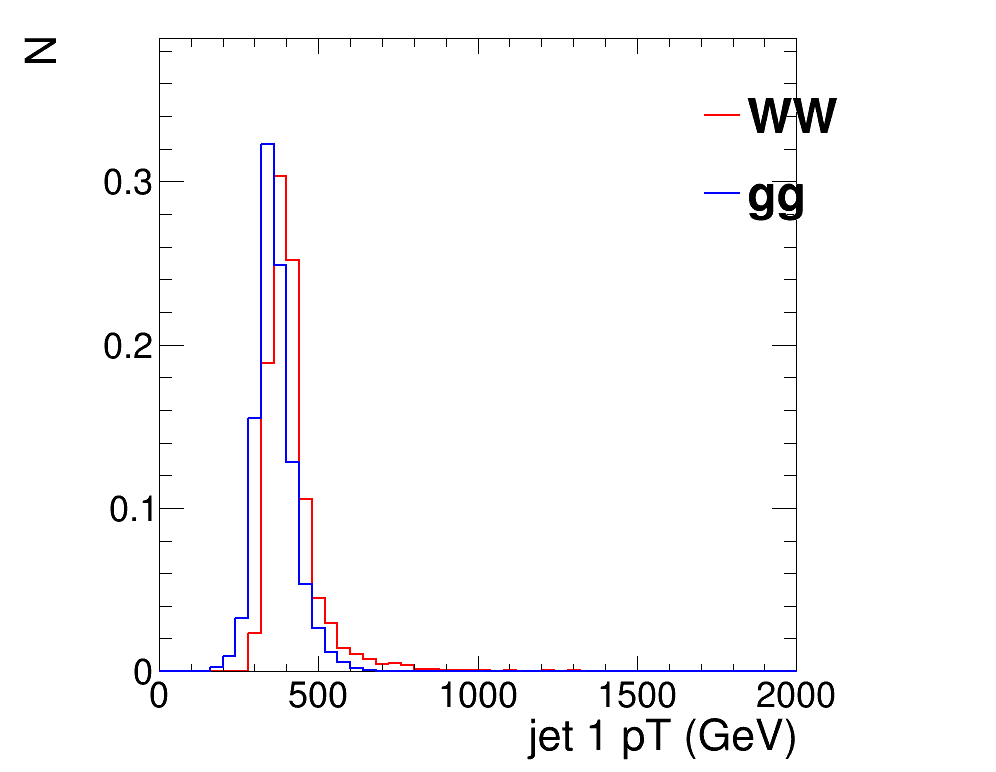
\includegraphics[width=0.48\textwidth]{./Figures/figs072514/figs071614_Wg_bin300_ak08/oneD/jpt1.png}}
\subfigure[\antikt R=1.2]{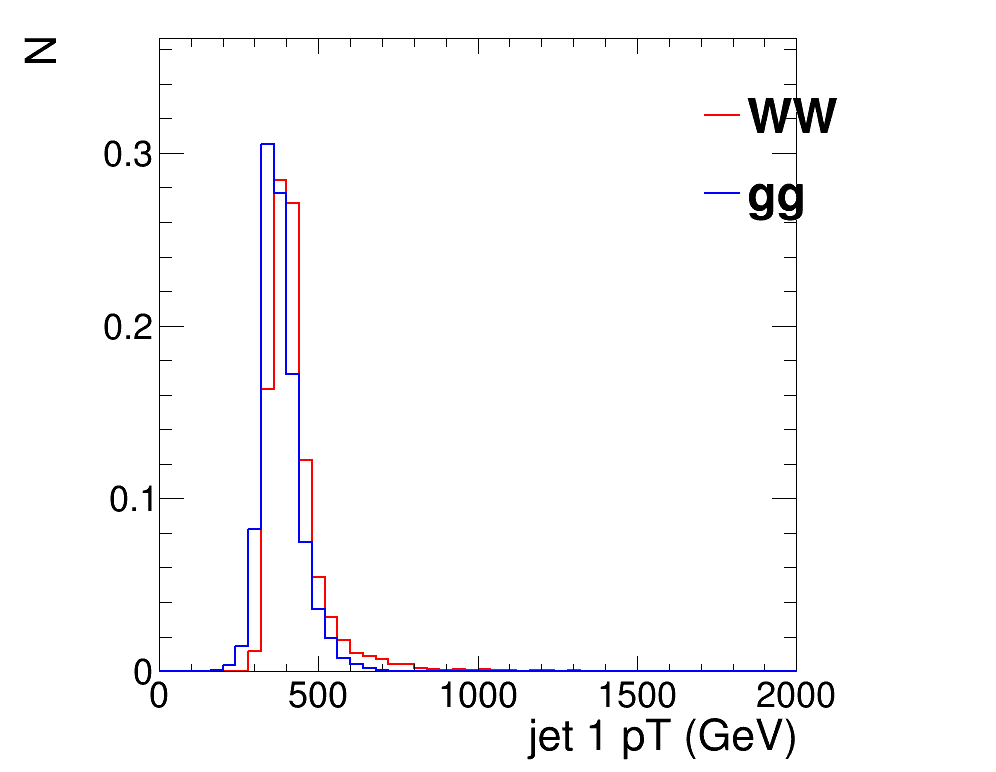
\includegraphics[width=0.48\textwidth]{./Figures/figs072514/figs071614_Wg_bin300_ak12/oneD/jpt1.png}}
\caption{Comparisons of the leading jet \pt spectrum of the $gg$
  background to the WW signal in the \pt 300-400 GeV bin using the
  different \antikt jet distance parameters explored.}
\label{fig:pt300_basics}
\end{center}
\end{figure*}

\begin{figure*}
\begin{center}
\subfigure[\antikt R=0.8]{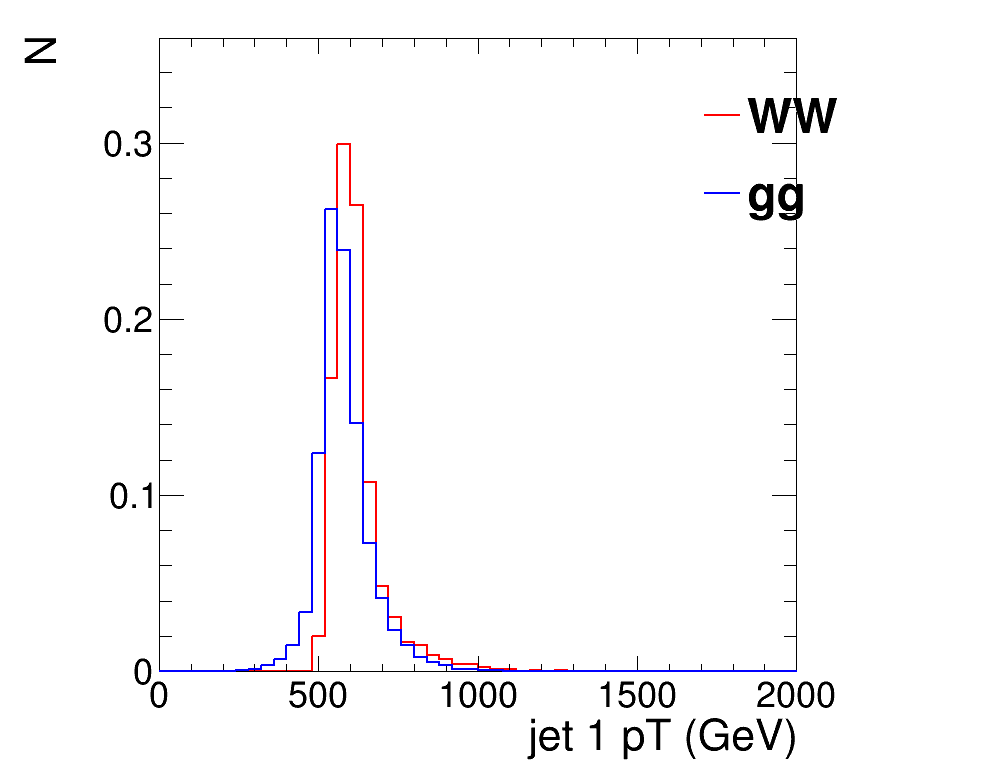
\includegraphics[width=0.48\textwidth]{./Figures/figs072514/figs071614_Wg_bin500_ak08/oneD/jpt1.png}}
\subfigure[\antikt R=1.2]{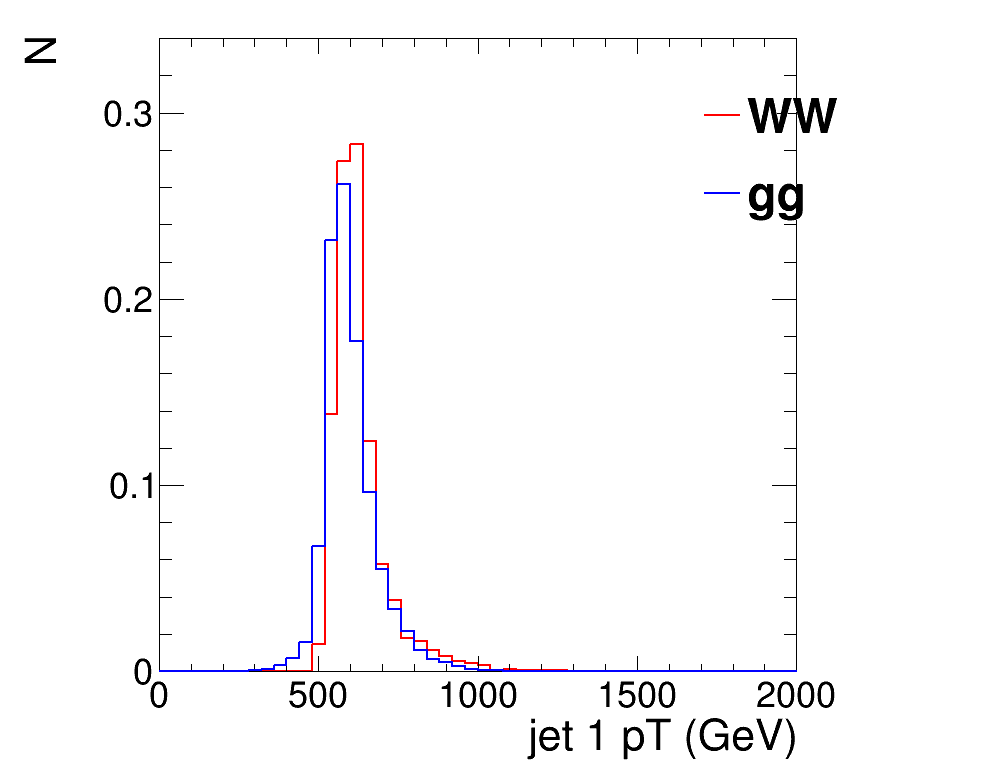
\includegraphics[width=0.48\textwidth]{./Figures/figs072514/figs071614_Wg_bin500_ak12/oneD/jpt1.png}}
\caption{Comparisons of the leading jet \pt spectrum of the $gg$
  background to the WW signal in the \pt 500-600 GeV bin using the
  different \antikt jet distance parameters explored.}
\label{fig:pt500_basics}
\end{center}
\end{figure*}

\begin{figure*}
\begin{center}
\subfigure[\antikt R=0.4]{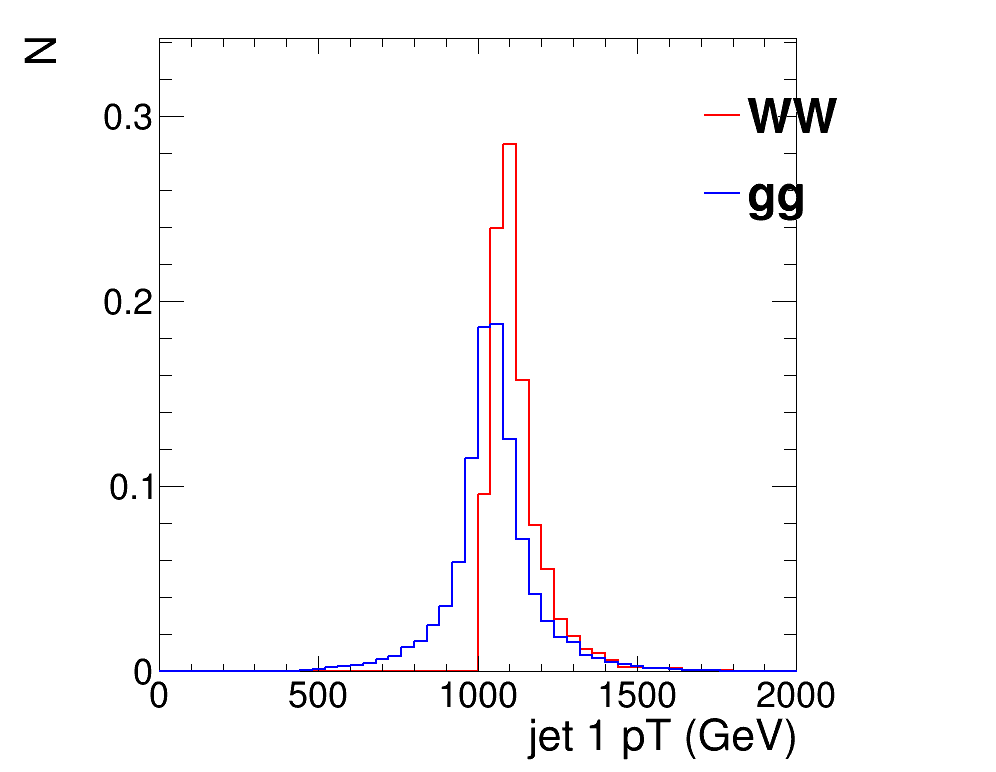
\includegraphics[width=0.48\textwidth]{./Figures/figs072514/figs071614_Wg_bin1000_ak04/oneD/jpt1.png}}
\subfigure[\antikt R=0.8]{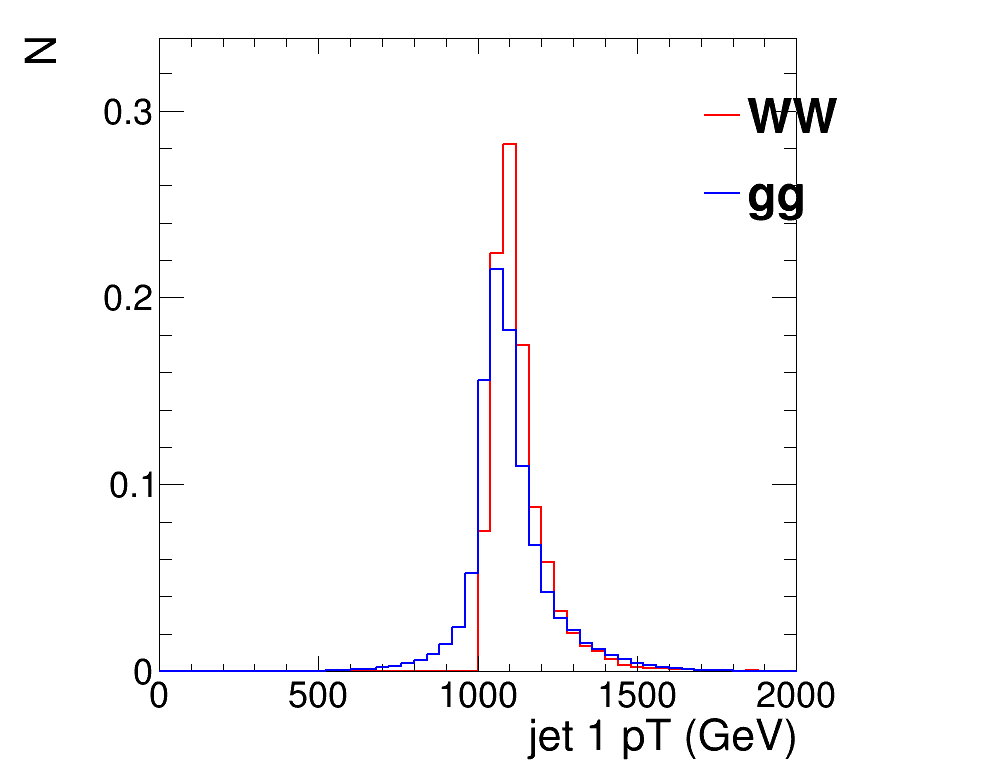
\includegraphics[width=0.48\textwidth]{./Figures/figs072514/figs071614_Wg_bin1000_ak08/oneD/jpt1.png}}
\subfigure[\antikt R=1.2]{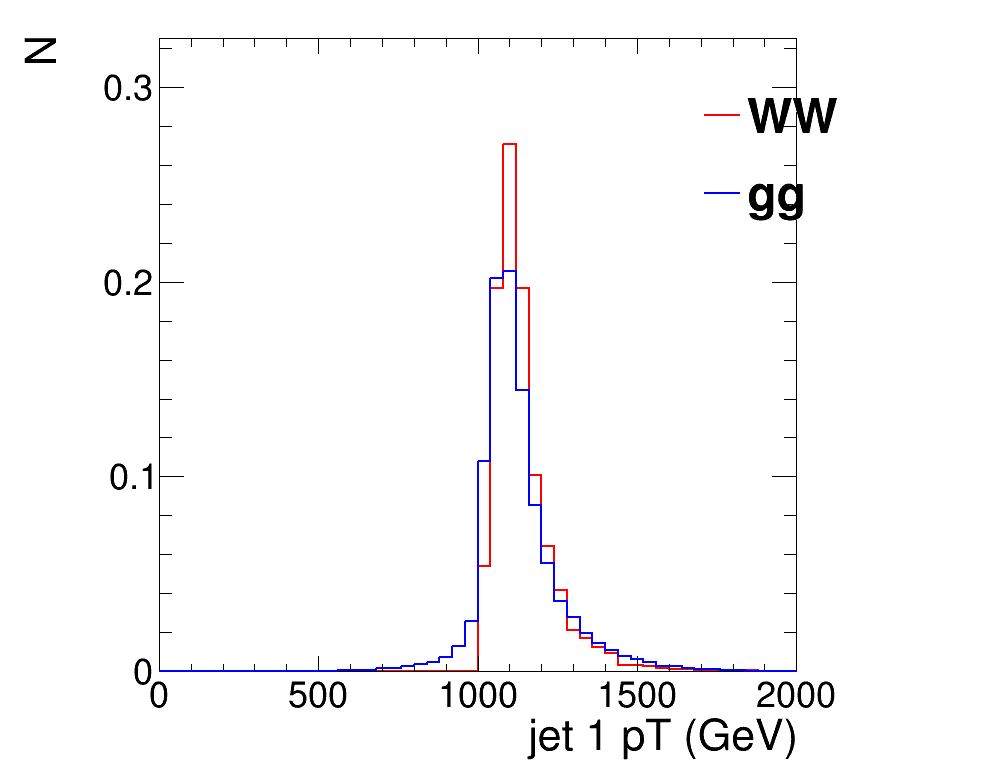
\includegraphics[width=0.48\textwidth]{./Figures/figs072514/figs071614_Wg_bin1000_ak12/oneD/jpt1.png}}
\caption{Comparisons of the leading jet \pt spectrum of the $gg$
  background to the WW signal in the \pt 1.0-1.1 TeV bin using the
  different \antikt jet distance parameters explored.}
\label{fig:pt1000_basics}
\end{center}
\end{figure*}


%\begin{figure*}
%\begin{center}
%\subfigure[Leading jet
%\pT]{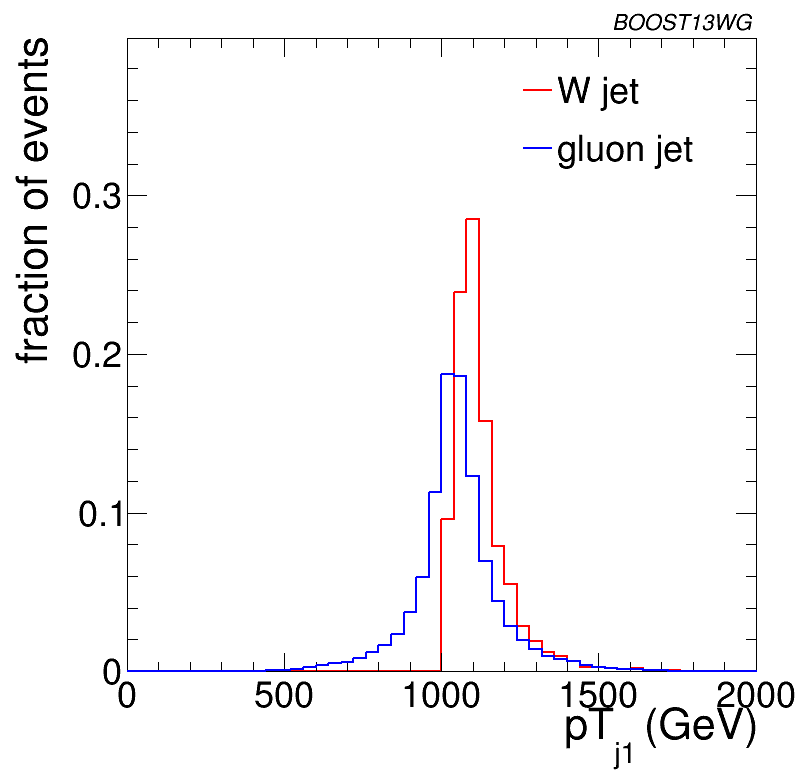
\includegraphics[width=0.48\textwidth]{./Figures/figs072514/figs071614_Wg_bin500_ak08/jpt1.png}}
%\subfigure[Sub-leading jet
%\pT]{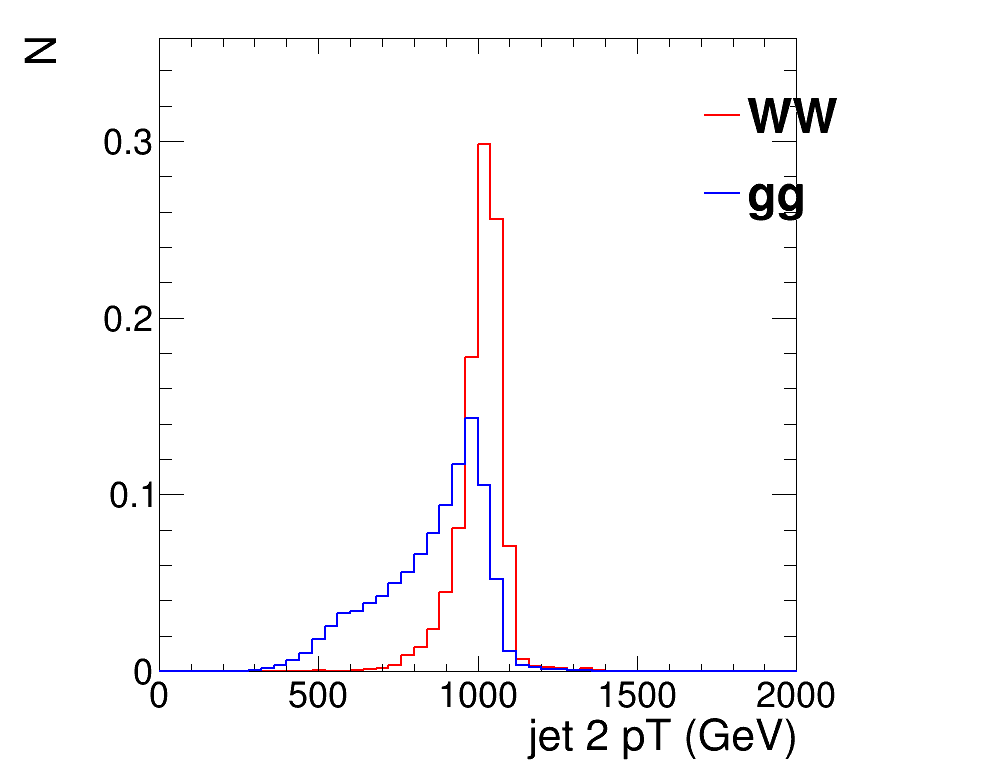
\includegraphics[width=0.48\textwidth]{./Figures/figs072514/figs071614_Wg_bin500_ak08/jpt2.png}}
%\subfigure[Leading jet
%$\eta$]{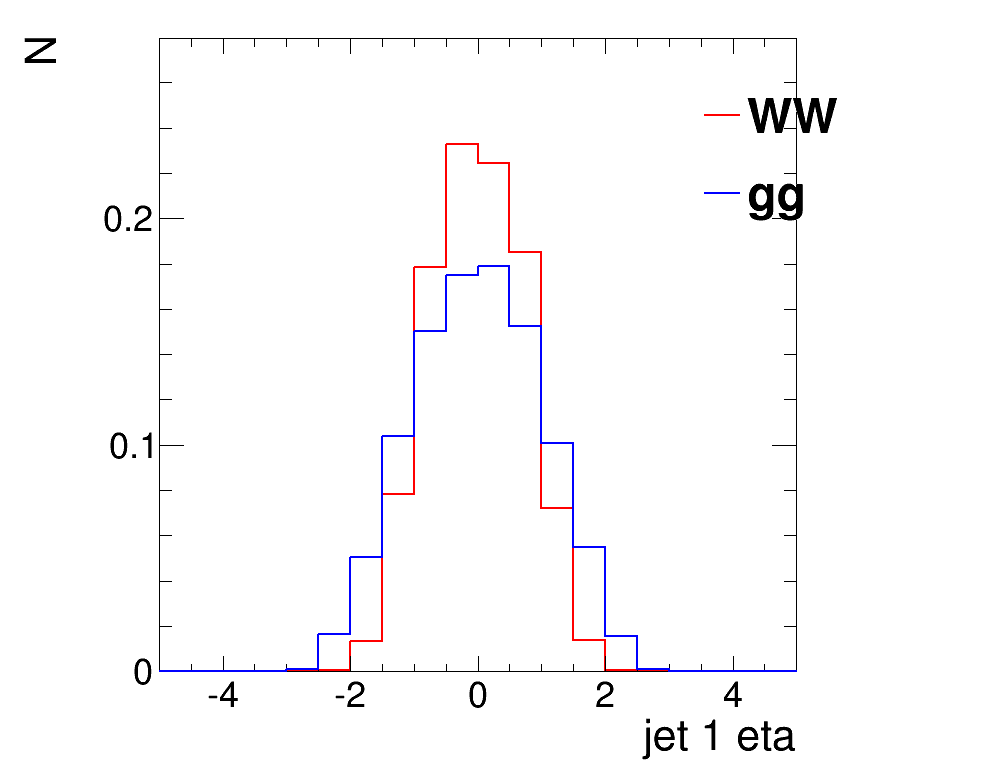
\includegraphics[width=0.48\textwidth]{./Figures/figs072514/figs071614_Wg_bin500_ak08/jeta1.png}}
%\subfigure[Sub-leading jet
%$\eta$]{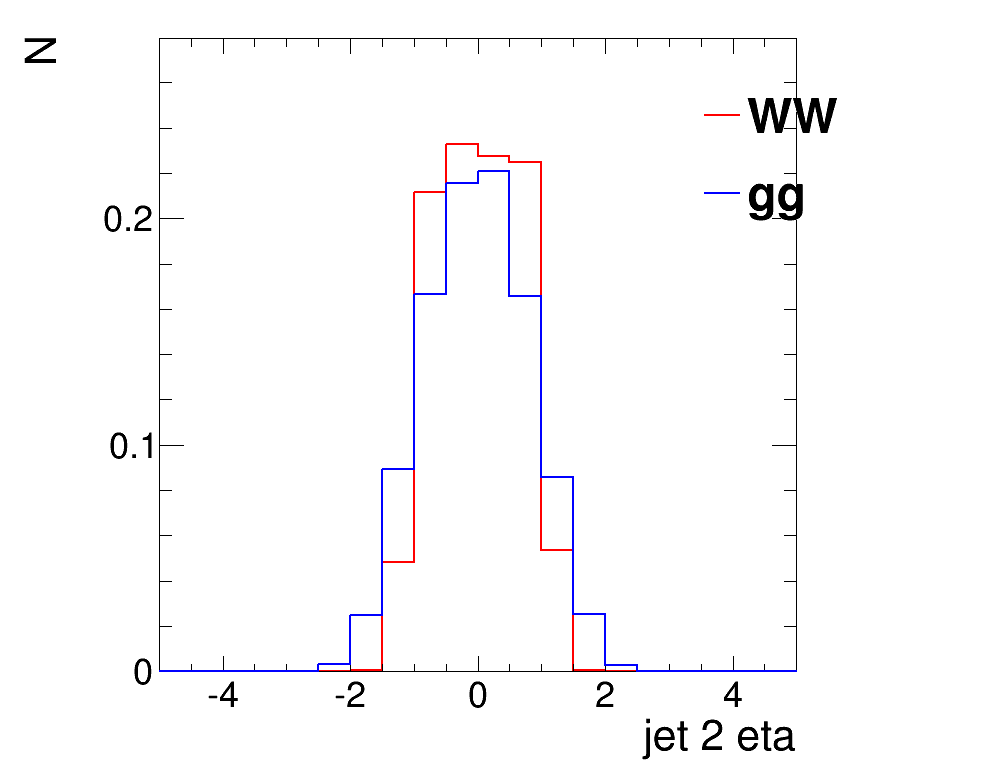
\includegraphics[width=0.48\textwidth]{./Figures/figs072514/figs071614_Wg_bin500_ak08/jeta2.png}}
%\caption{Comparisons of the QCD background to the WW signal in the \pt 500 GeV bin using the anti-\kT R=0.8 algorithm: basic
%  kinematic distributons.}
%\label{fig:pt500_basics_AKt_R08}
%\end{center}
%\end{figure*}



\subsection{Single Variable Performance}

In this section we will explore the performance of the various groomed
jet mass and substructure variables in terms of discriminating signal
and background, and how this performance changes depending on the
kinematic bin and jet radius considered.

Figure~\ref{fig:pt500_mass_AKt_R08} the compares the signal and
background in terms of the different groomed masses explored for the
\antikt R=0.8 algorithm in the \pt 500-600 bin. One can clearly see
that in terms of separating signal and background the groomed masses
will be significantly more performant than the ungroomed \antikt R=0.8
mass. {\it Need to comment on the soft drop B=-1 mass here}
Figure~\ref{fig:pt500_subst_AKt_R08}
compares signal and background in the different substructure variables
explored for the same jet radius and kinematic bin. 

\begin{figure*}
\begin{center}
\subfigure[Ungroomed mass]{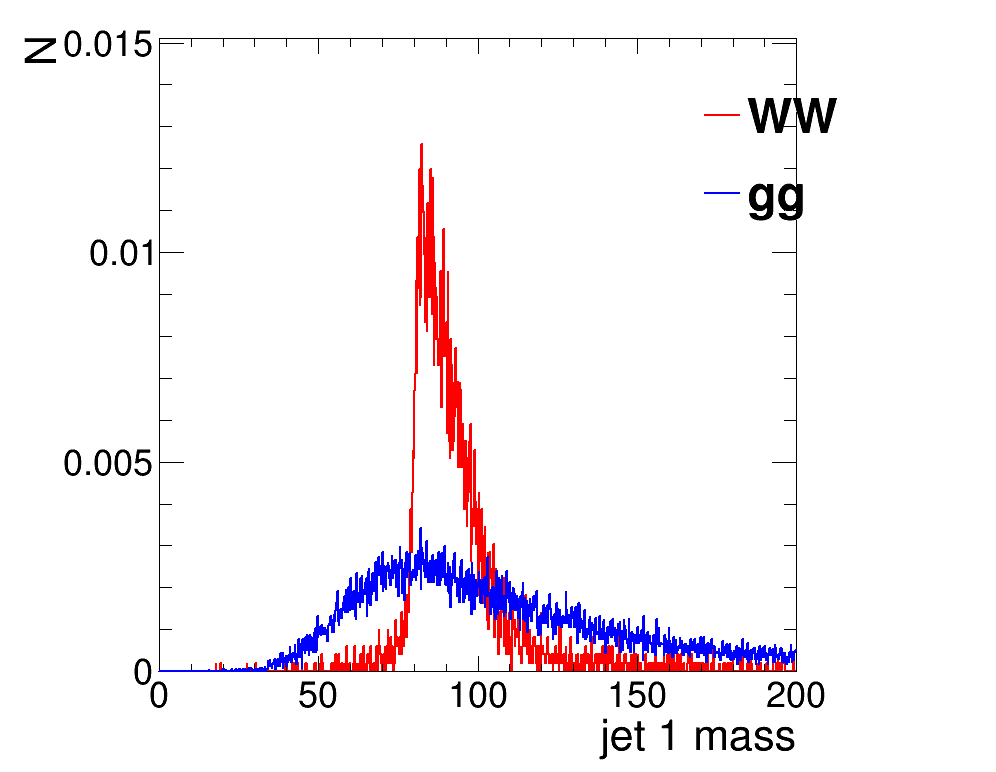
\includegraphics[width=0.48\textwidth]{./Figures/figs072514/figs071614_Wg_bin500_ak08/oneD/jmass1.png}}
\subfigure[Pruned mass]{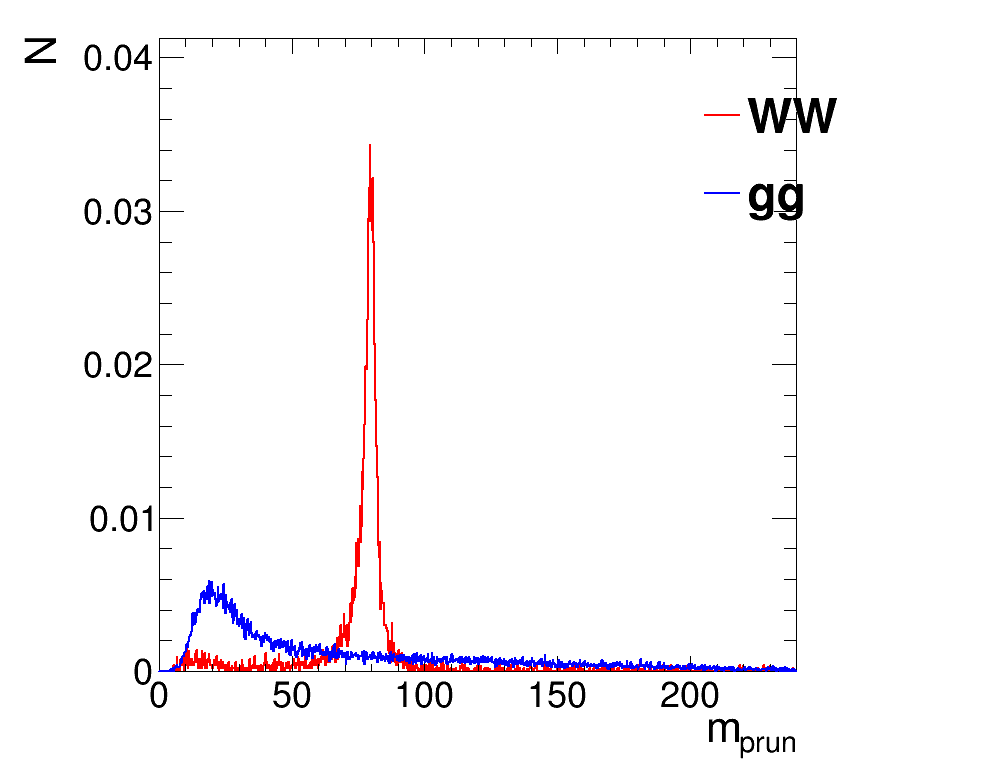
\includegraphics[width=0.48\textwidth]{./Figures/figs072514/figs071614_Wg_bin500_ak08/oneD/h_mass_prun.png}}
\subfigure[Trimmed mass]{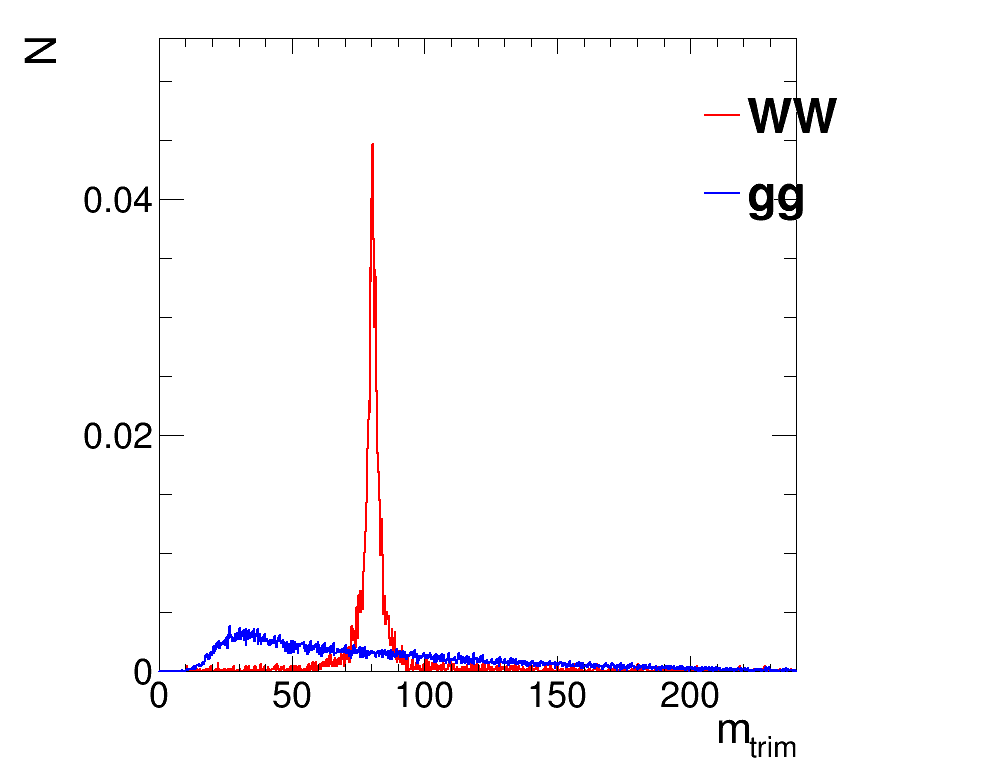
\includegraphics[width=0.48\textwidth]{./Figures/figs072514/figs071614_Wg_bin500_ak08/oneD/h_mass_trim.png}}
\subfigure[mMDT mass]{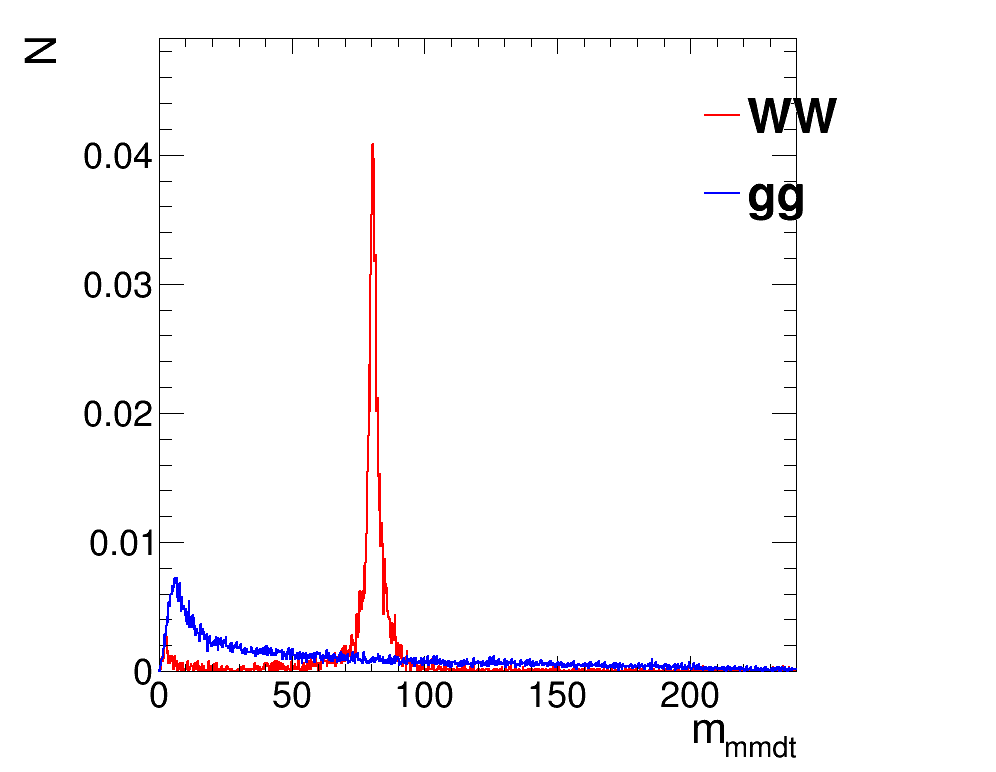
\includegraphics[width=0.48\textwidth]{./Figures/figs072514/figs071614_Wg_bin500_ak08/oneD/h_mass_mmdt.png}}
\subfigure[Soft-drop $\beta=2$ mass]{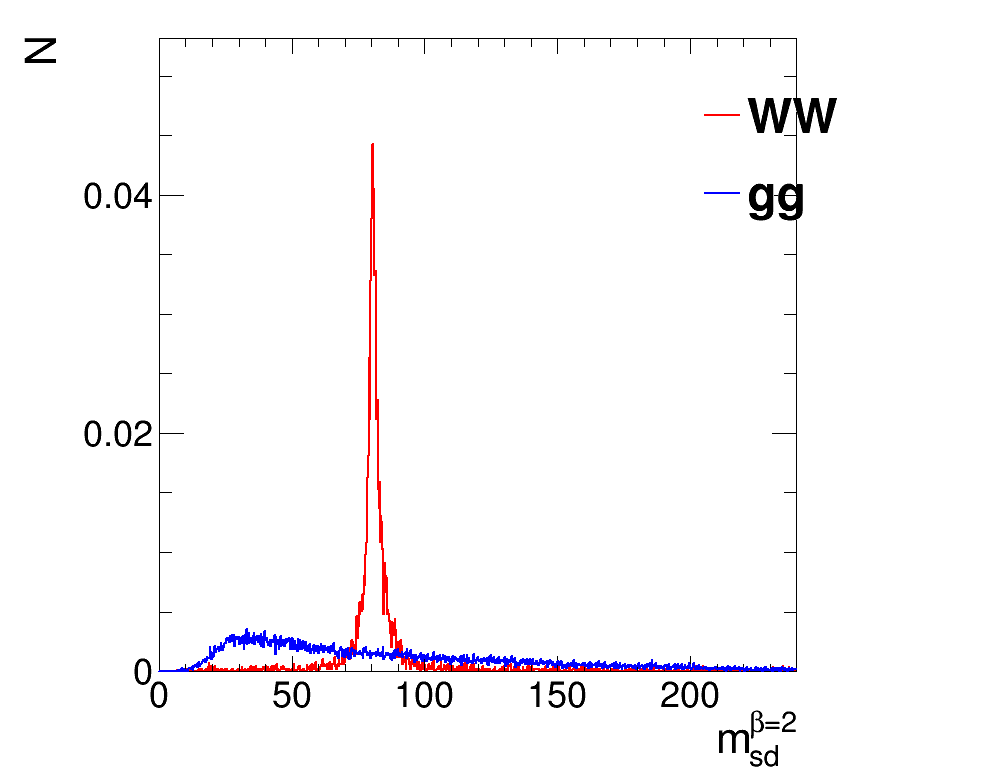
\includegraphics[width=0.48\textwidth]{./Figures/figs072514/figs071614_Wg_bin500_ak08/oneD/h_mass_sdb2.png}}
%\subfigure[Soft-drop $\beta=-1$ mass]{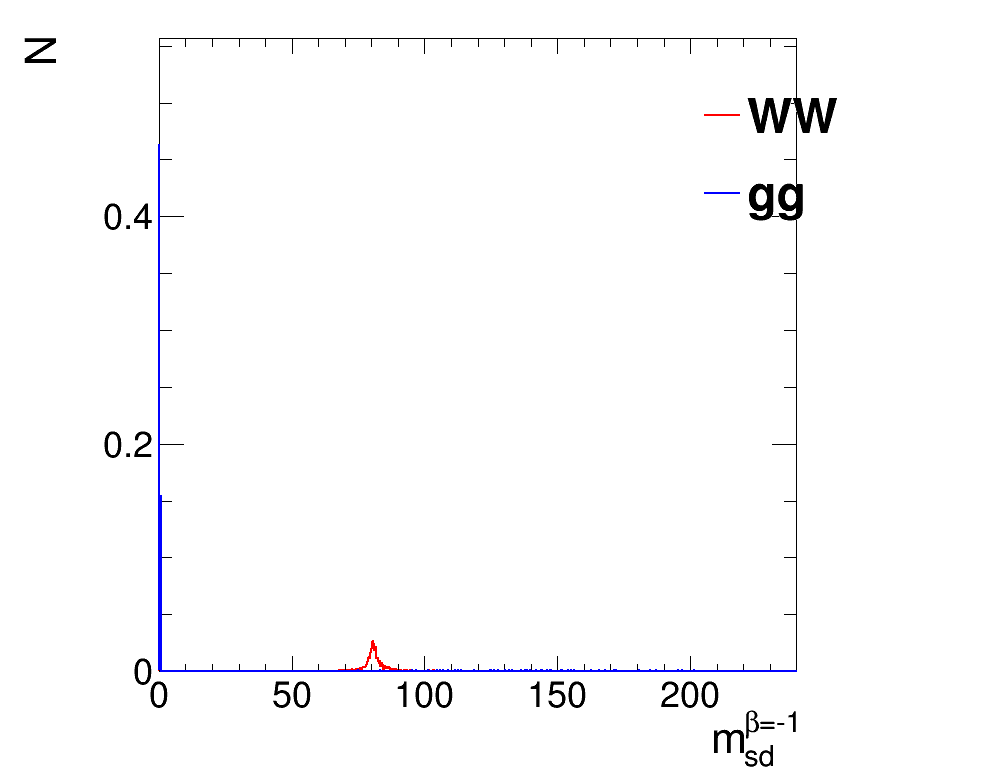
\includegraphics[width=0.48\textwidth]{./Figures/figs072514/figs071614_Wg_bin500_ak08/oneD/h_mass_sdm1.png}}
\caption{Comparisons of the QCD background to the WW signal in the \pt 500-600 GeV bin using the anti-\kT R=0.8 algorithm: leading
  jet mass distributions.}
\label{fig:pt500_mass_AKt_R08}
\end{center}
\end{figure*}

\begin{figure*}
\begin{center}
\subfigure[$C_2^{\beta=1}$]{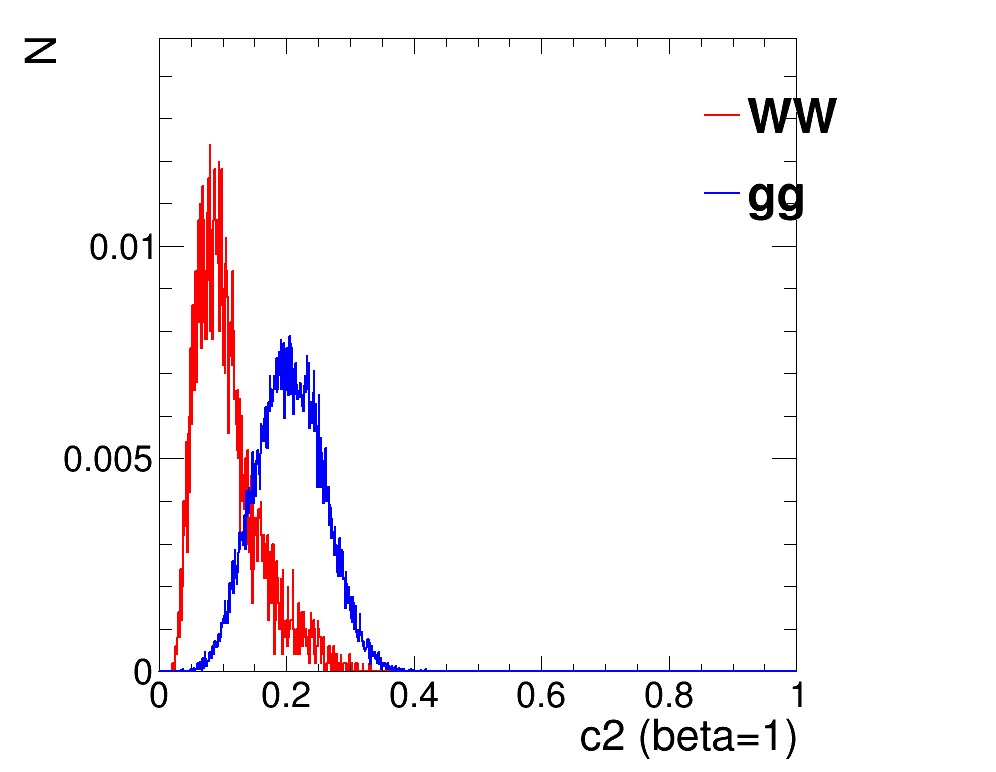
\includegraphics[width=0.48\textwidth]{./Figures/figs072514/figs071614_Wg_bin500_ak08/oneD/h_c2_b1.png}}
\subfigure[$C_2^{\beta=2}$]{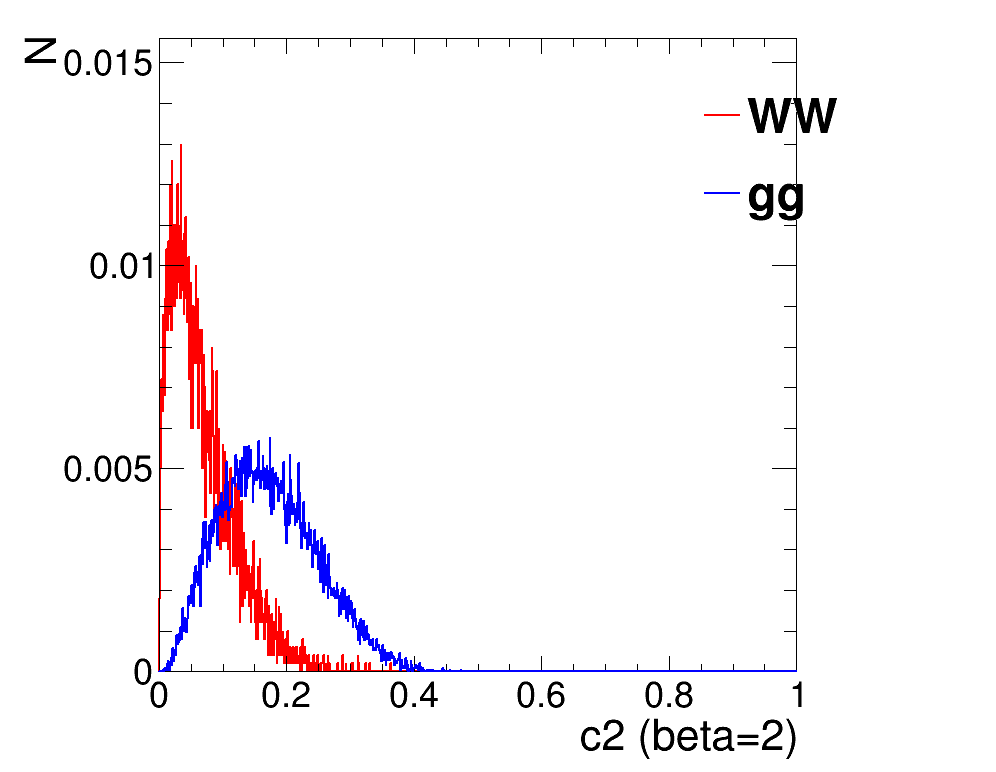
\includegraphics[width=0.48\textwidth]{./Figures/figs072514/figs071614_Wg_bin500_ak08/oneD/h_c2_b2.png}}
\subfigure[$\Gamma_{Qjet}$]{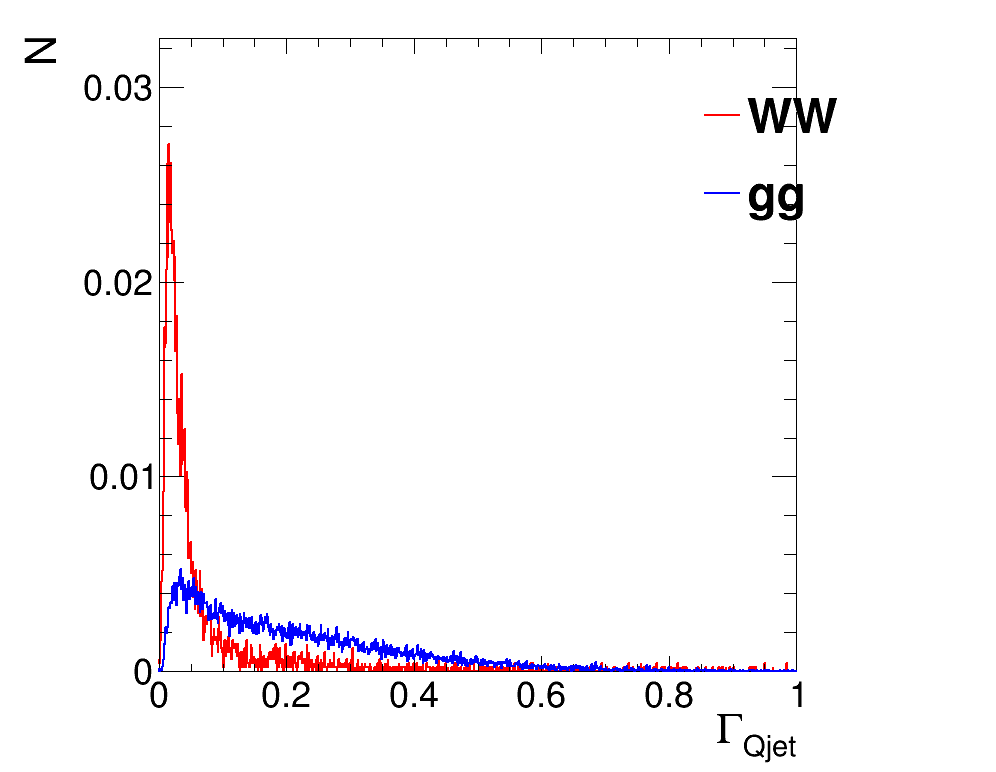
\includegraphics[width=0.48\textwidth]{./Figures/figs072514/figs071614_Wg_bin500_ak08/oneD/h_qjetVol.png}}
\subfigure[$\tau_{21}^{\beta=1}$]{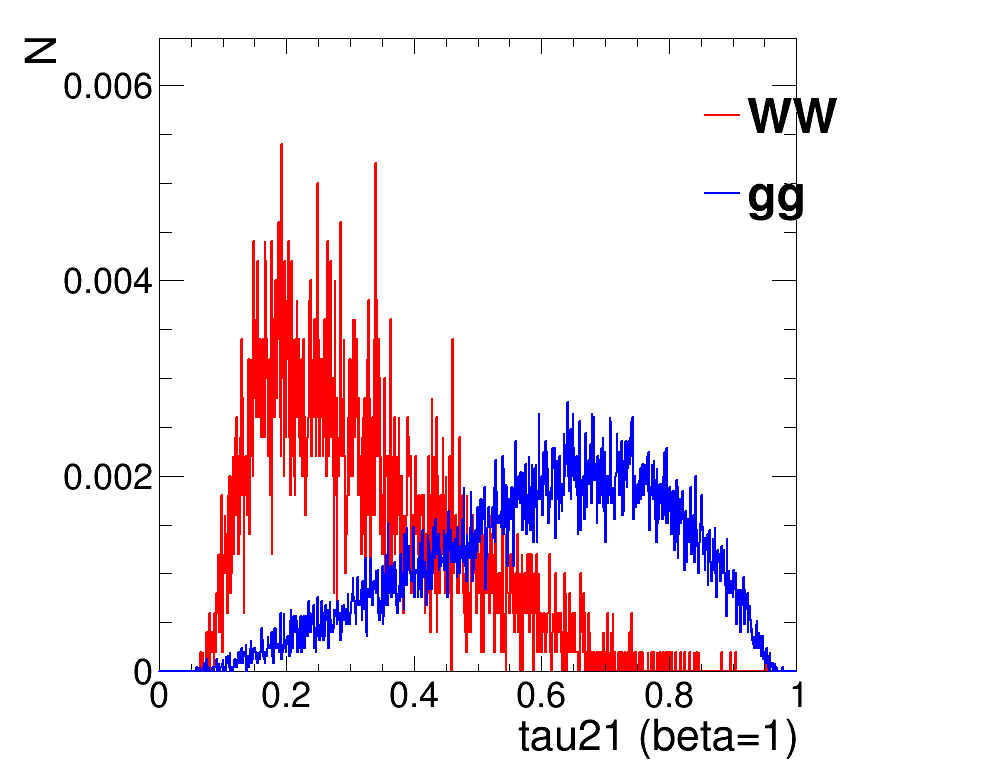
\includegraphics[width=0.48\textwidth]{./Figures/figs072514/figs071614_Wg_bin500_ak08/oneD/h_tau21_b1.png}}
\subfigure[$\tau_{21}^{\beta=2}$]{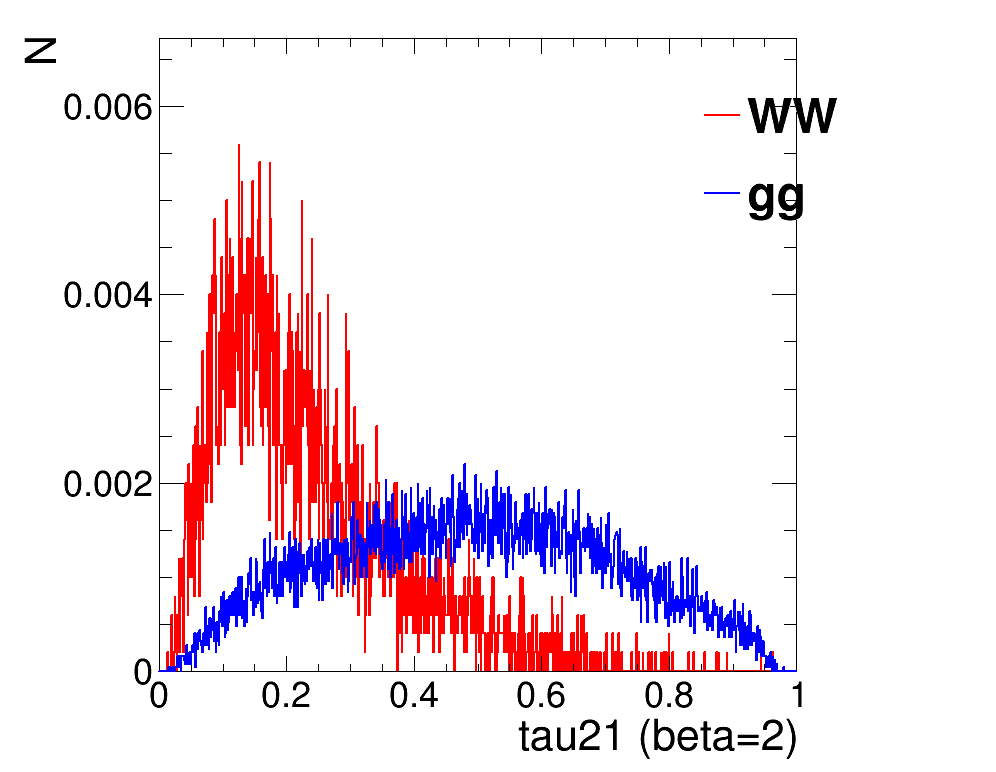
\includegraphics[width=0.48\textwidth]{./Figures/figs072514/figs071614_Wg_bin500_ak08/oneD/h_tau21_b2.png}}
\caption{Comparisons of the QCD background to the WW signal in the \pt 500-600 GeV bin using the anti-\kT R=0.8 algorithm:
  substructure variables.}
\label{fig:pt500_subst_AKt_R08}
\end{center}
\end{figure*}


Figures~\ref{fig:pt300_single},\ref{fig:pt500_single}
and~\ref{fig:pt1000_single} show the single variable ROC curves
compared to the ROC curve for a BDT combination of all the variables
(labelled ``allvars''),
for each of the \antikt distance parameters considered in each of the
kinematic bins. One can see that, in all cases, the ``allvars'' option
is considerably more performant than any of the individual single variables
considered, indicating that there is considerable complimentarity
between the variables, that will be explored further in the next
section. The best performant individual variables for a reasonable signal
efficiency are the groomed masses, which all have a similar
level of performance that is superior to that of any of the
substructure variables considered. 
%Comparing the impact of increasing the jet
%radius in the same kinematic bin, one can see that the groomed mass
%performance does not vary greatly, but that the performance of the
%substructure variables is markedly worse for larger jet radius.



%At low pT, substructure performance gets worse across the board as radius increases
%In Figure~\ref{fig:pt500_comb2D}  we can also
%observe that the degradation of the substructure variable performance
%with increased jet radius is not uniform. The background rejection of
%$C_2^{\beta=1}$ degrades substantially more than that of
%$\tau_{21}^{\beta=1}$ as the 
%At highest pT, the situation is different again....

% when you are at the characteristic scale of the jet, C2B1 does well,
% but when it is wider than necessaruy it starts to fail

%Figure~\ref{fig:pt500_single_AKt_R08} shows the single variable ROC curves in
%the \pT 500 GeV bin for the anti-\kT R=0.8 algorithm, compared to the
%ROC curve for a BDT combination of all the variables. One can see that
%the best performant single variables for a reasonable signal
%efficiency are the groomed/filtered masses, which all have a similar
%level of performance with the exception of the soft drop mass with $\beta=-1$. {\it Would be good to split this into two plots, one
%using the masses and one for other variables, or somehow make the mass
%and other variable curves more distinct from one another by using same
%colour for all the mass curves}.
%
%{\it We want to look also at:
%\begin{itemize}
%\item Dependence on R. So have the same single variable ROC for
%e.g. R=1.2, R=0.4. Then possibly have another plot which compares the
%best single variable (e.g. groomed mass) for
%different R.
%\item Dependence on pT. Again want to repeat the plot for different
%kinematic bins, and then have a plot which compares the best
%performance in each kinematic bin to see the dependence of performance
%on kinematics.
%\end{itemize}
%}

\begin{figure*}
\begin{center}
\subfigure[\antikt R=0.8, \pt 300-400 GeV bin]{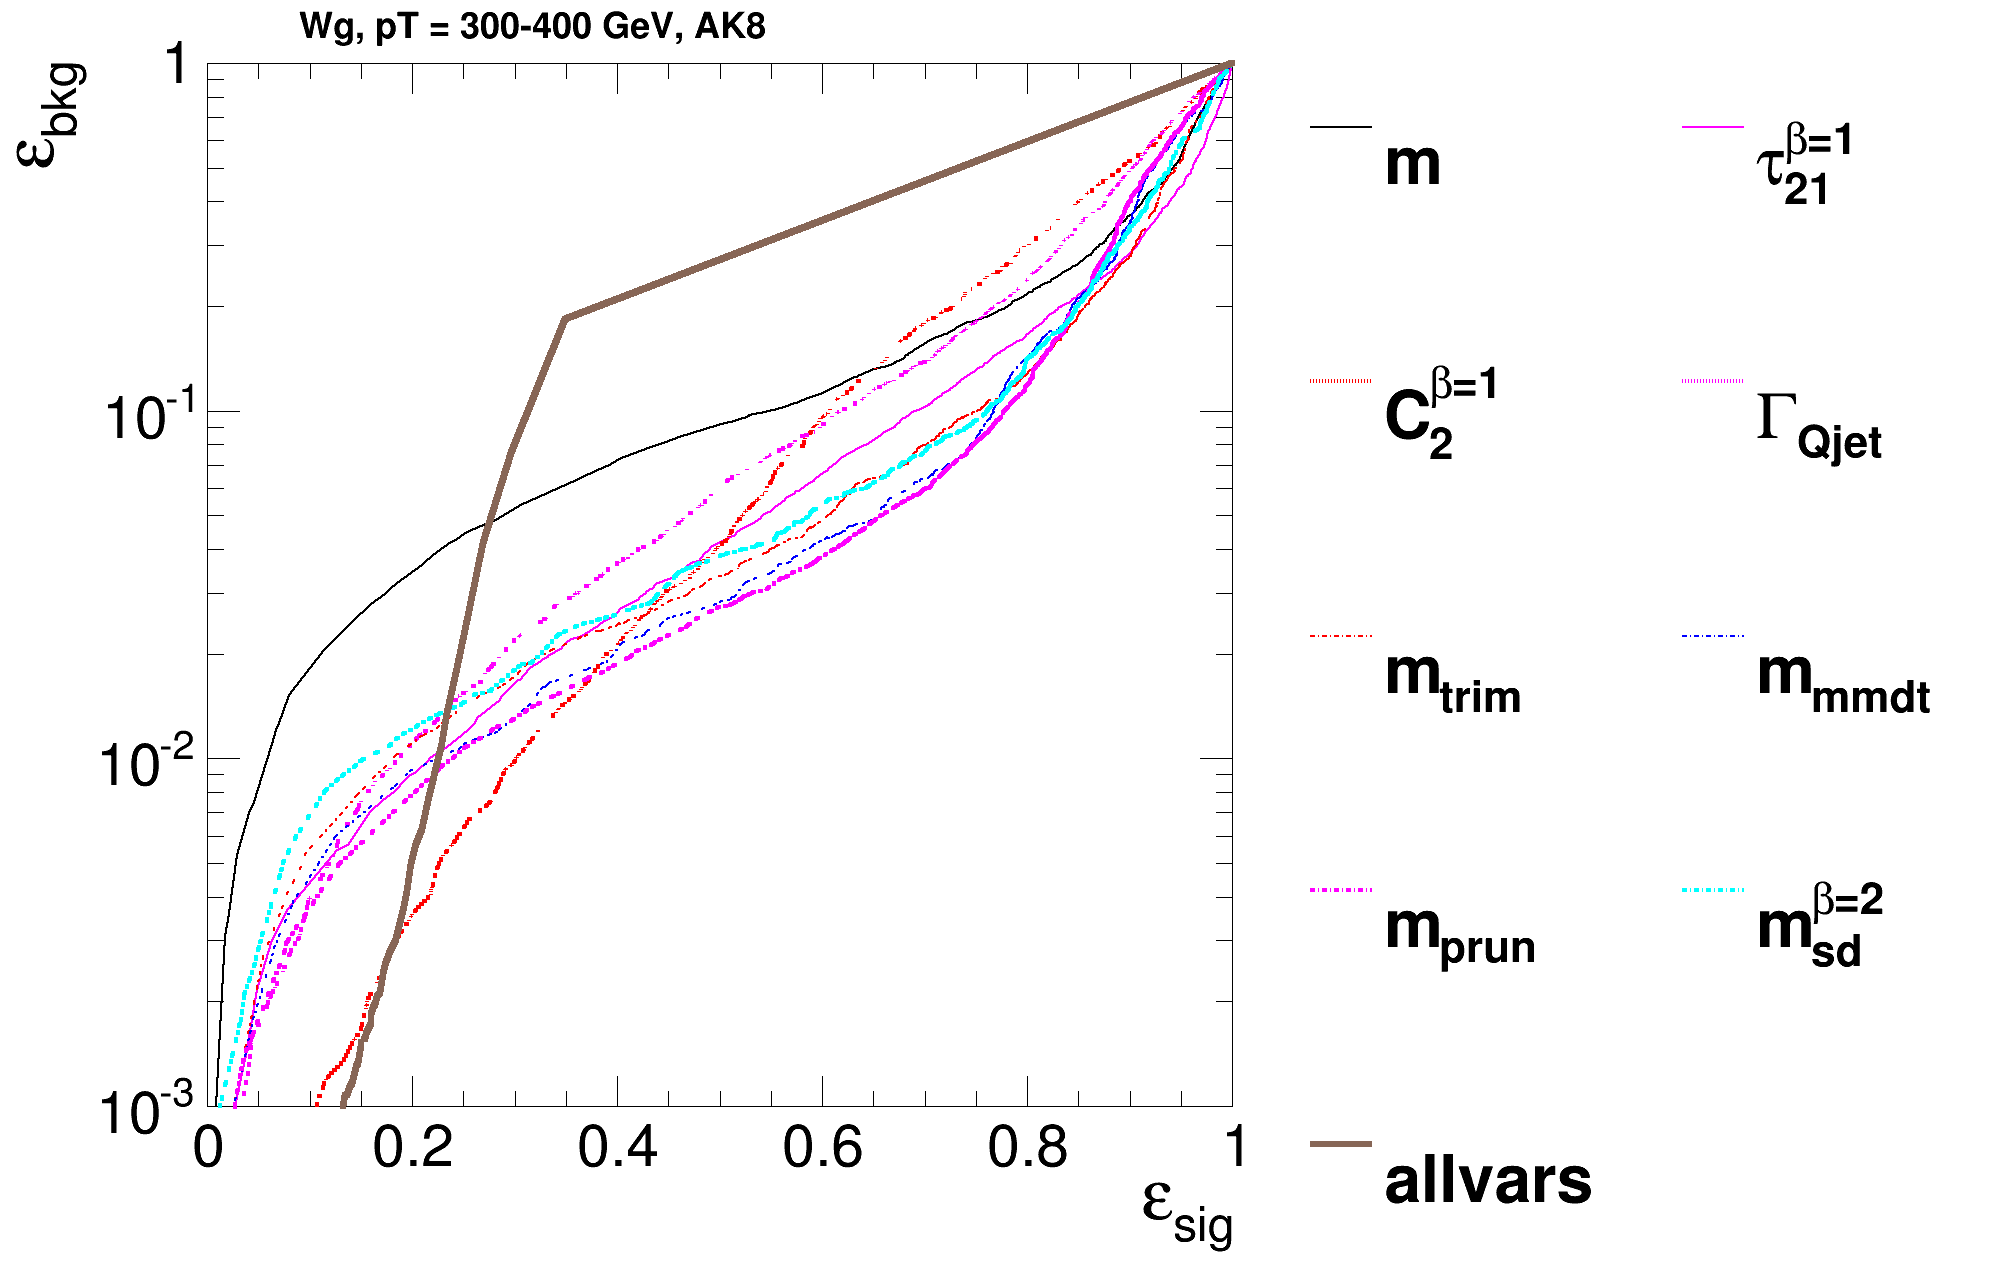
\includegraphics[width=0.7\textwidth]{./Figures/figs072514/figs071614_Wg_bin300_ak08/rocs/Rocs_1D_single.png}}
\subfigure[\antikt R=1.2, \pt 300-400 GeV bin]{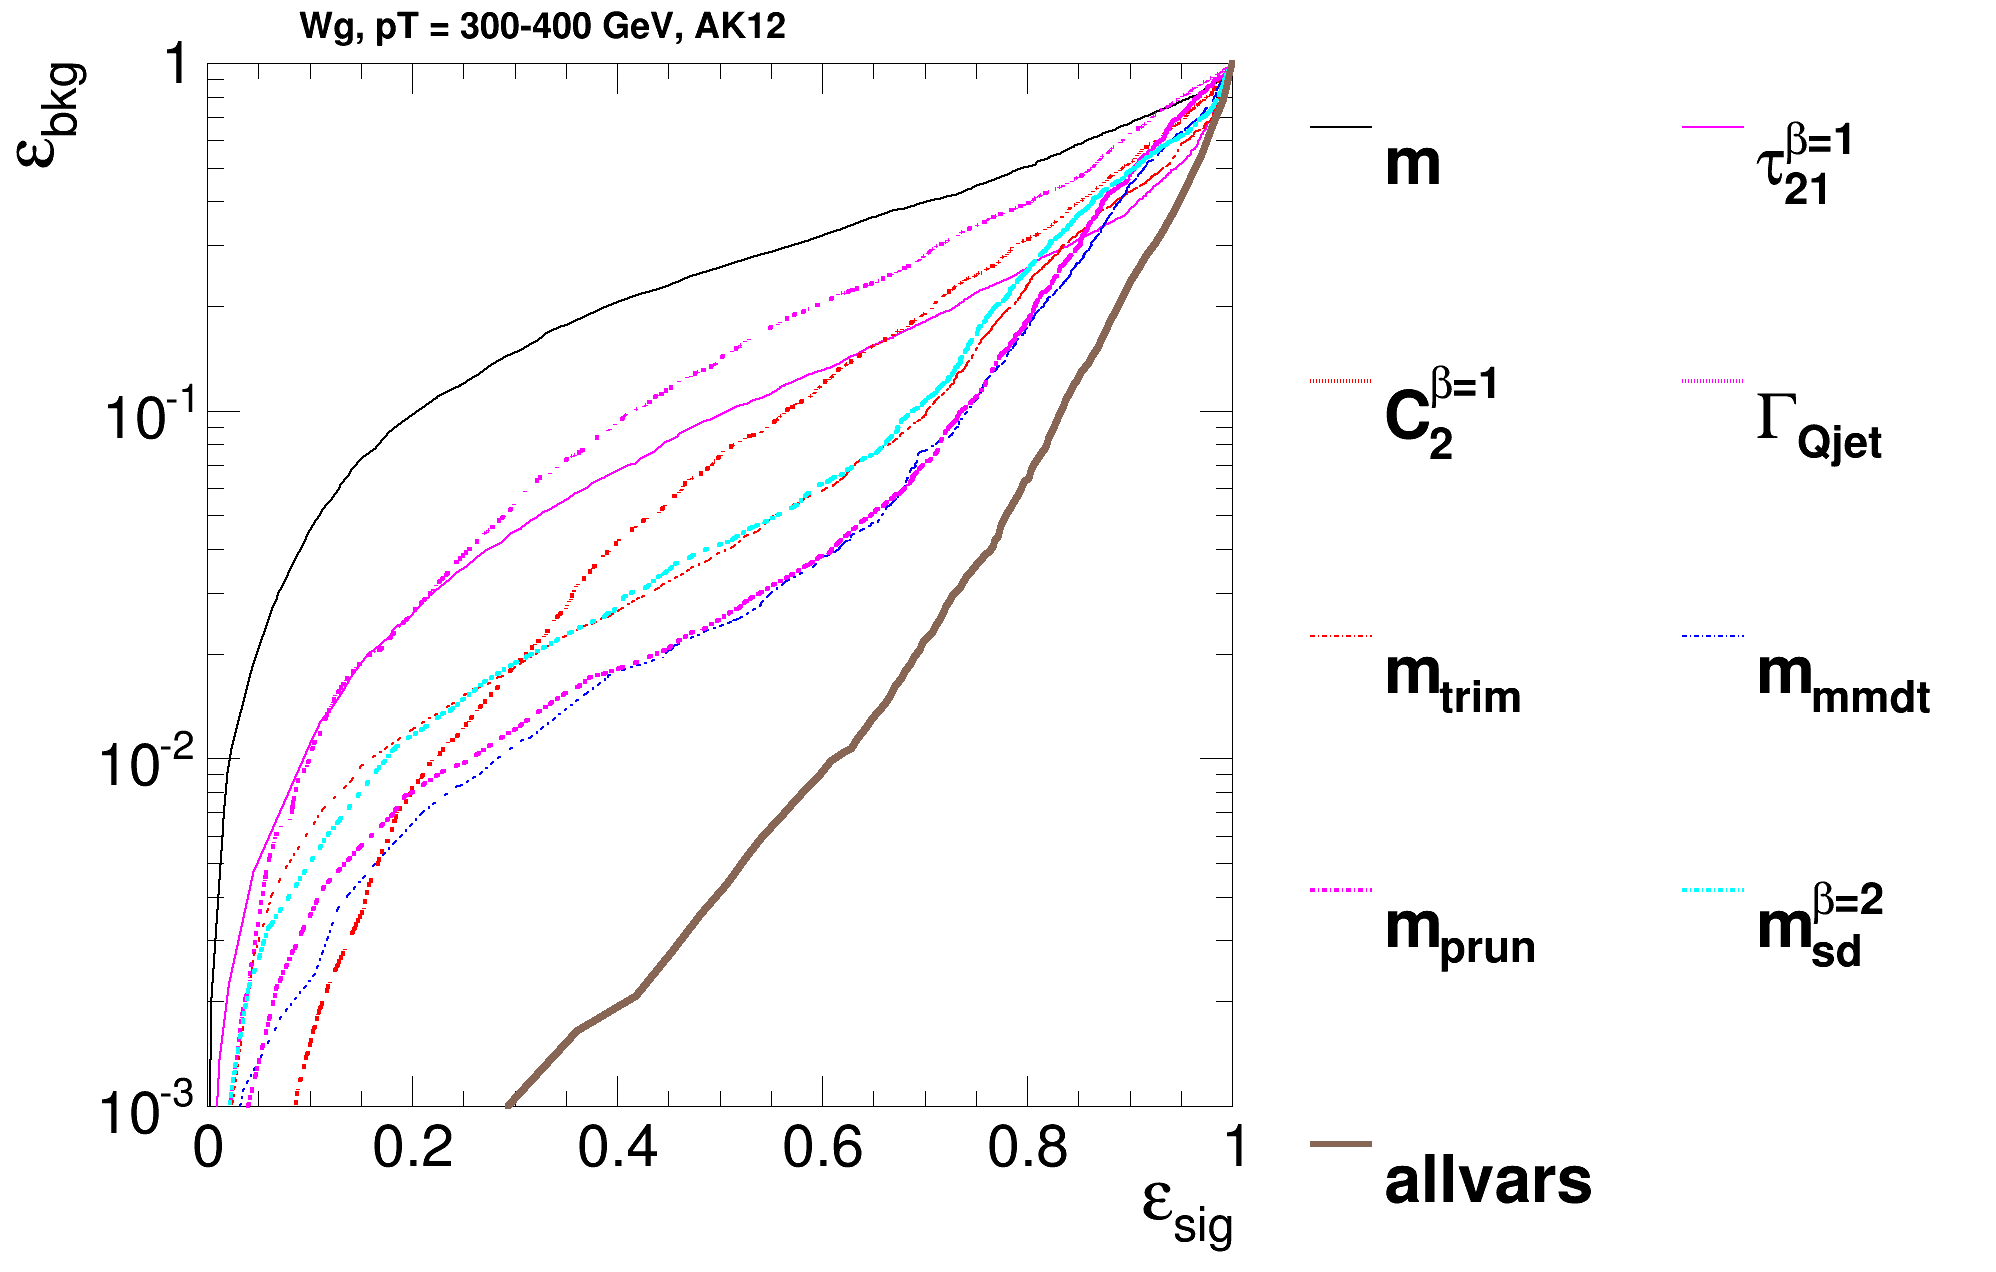
\includegraphics[width=0.7\textwidth]{./Figures/figs072514/figs071614_Wg_bin300_ak12/rocs/Rocs_1D_single.png}}
\caption{The ROC curve for all single variables considered for $W$
tagging in the \pt 300-400 GeV bin using the anti-\kT R=0.8 algorithm
(top) and R=1.2 algorithm (bottom).}
\label{fig:pt300_single}
\end{center}
\end{figure*}


\begin{figure*}
\begin{center}
\subfigure[\antikt R=0.8, \pt 500-600 GeV bin]{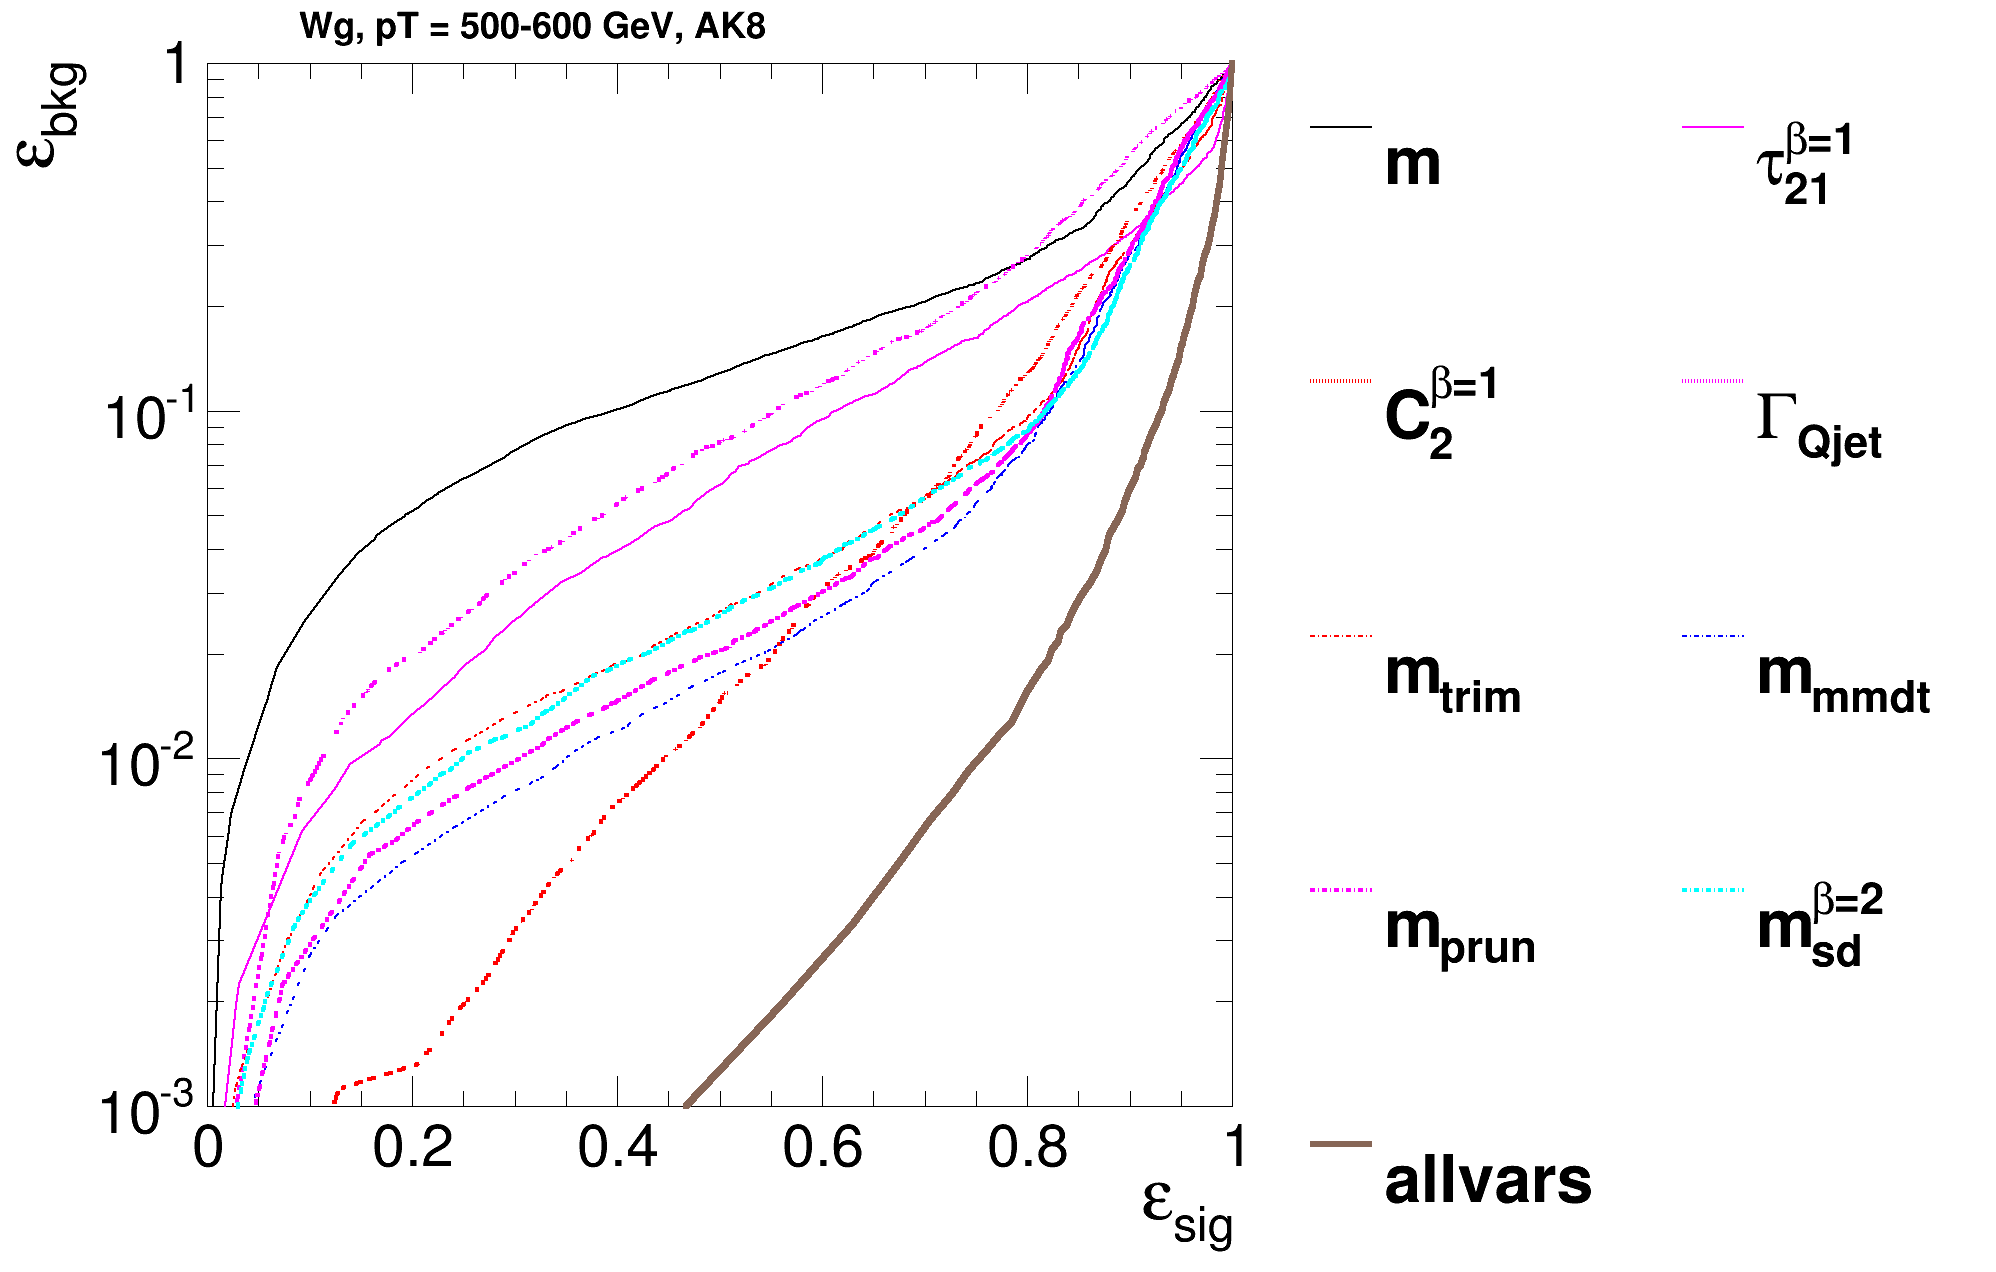
\includegraphics[width=0.7\textwidth]{./Figures/figs072514/figs071614_Wg_bin500_ak08/rocs/Rocs_1D_single.png}}
\subfigure[\antikt R=1.2, \pt 500-600 GeV bin]{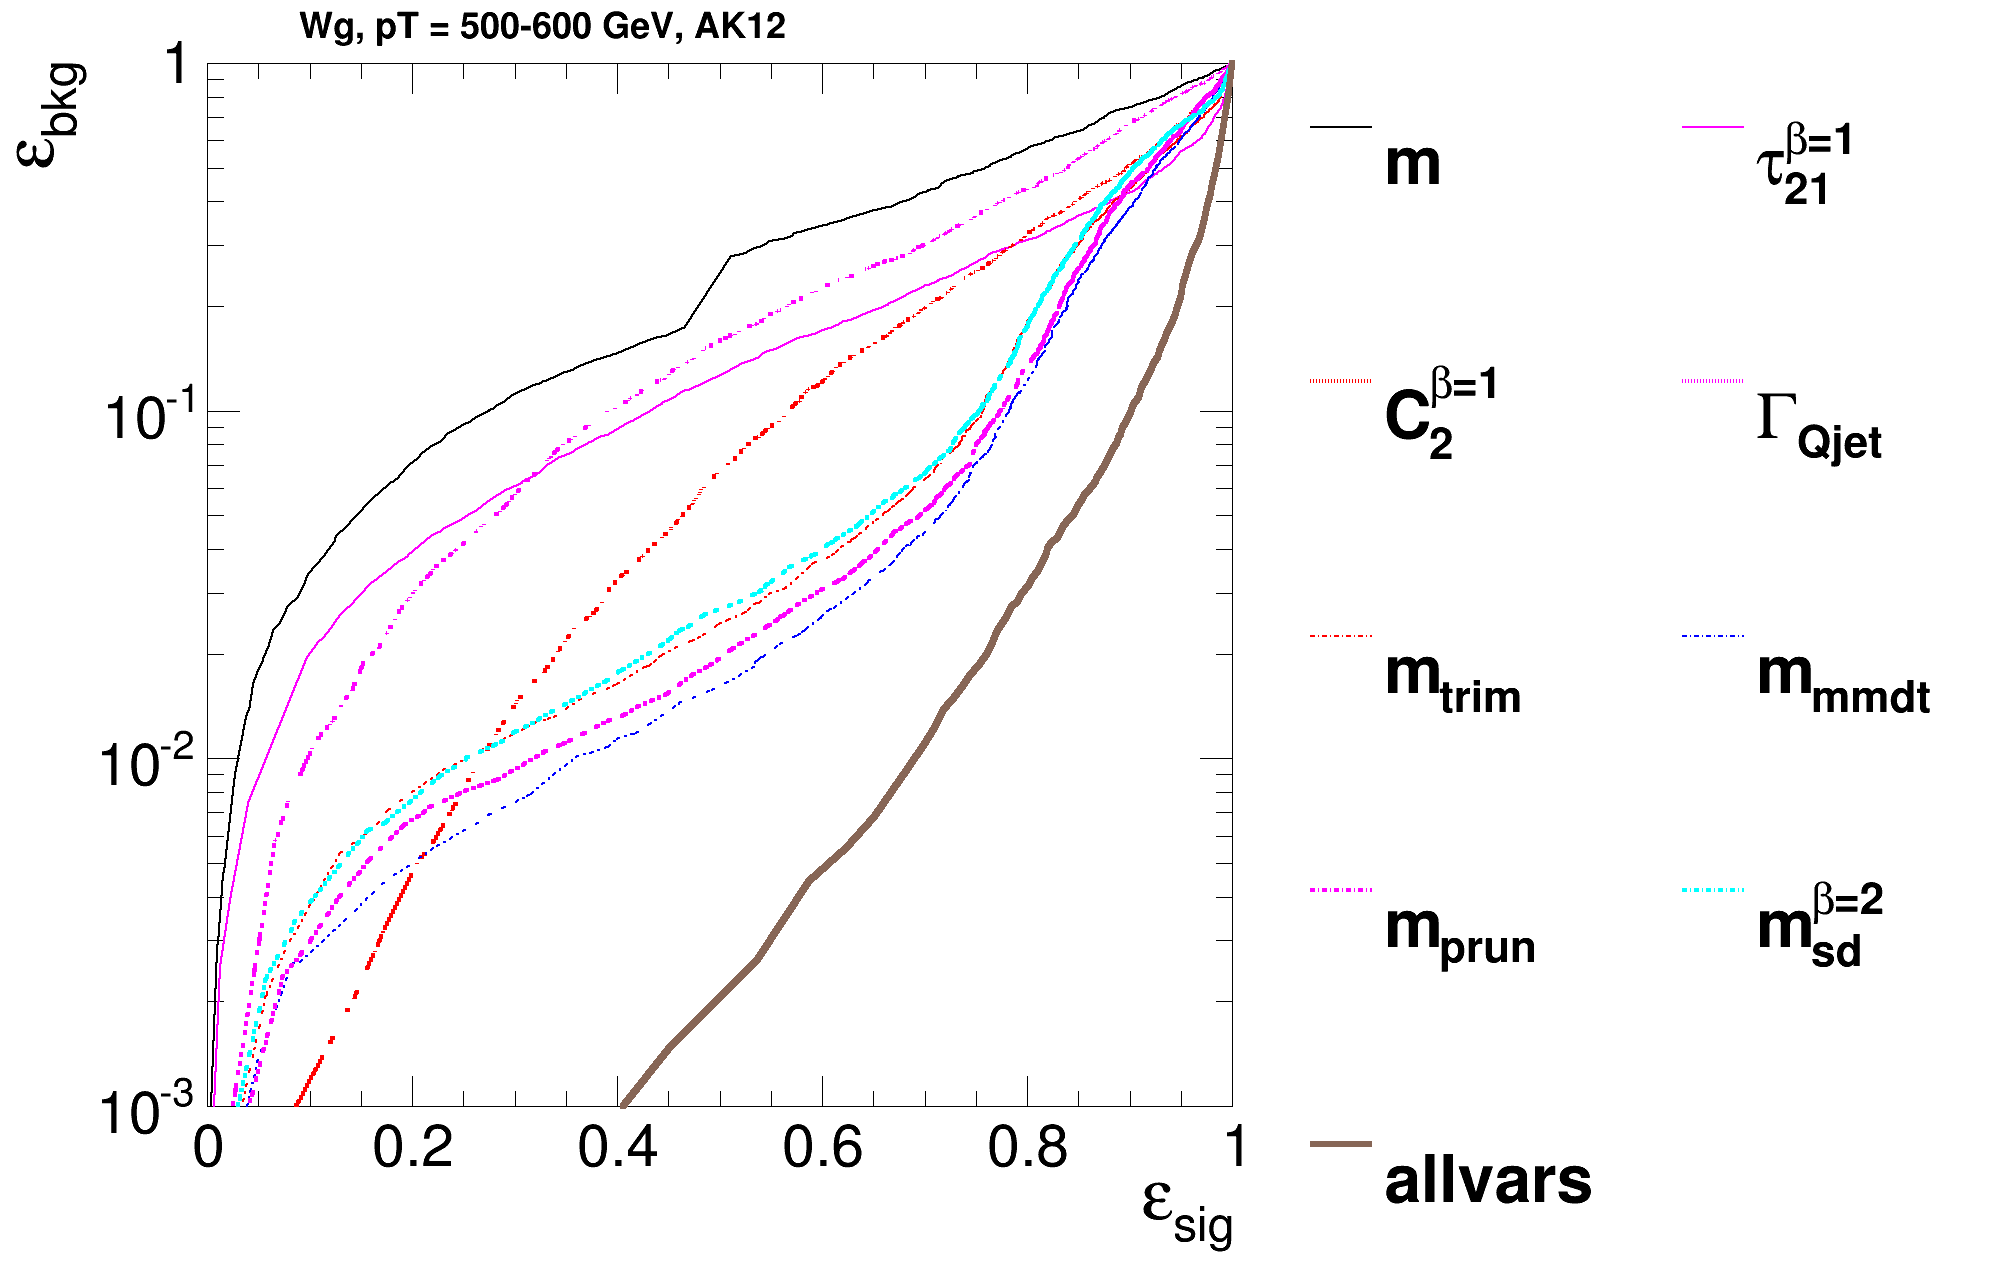
\includegraphics[width=0.7\textwidth]{./Figures/figs072514/figs071614_Wg_bin500_ak12/rocs/Rocs_1D_single.png}}
\caption{The ROC curve for all single variables considered for $W$
tagging in the \pt 500-600 GeV bin using the anti-\kT R=0.8 algorithm
(top) and R=1.2 algorithm (bottom).}
\label{fig:pt500_single}
\end{center}
\end{figure*}

\begin{figure*}
\begin{center}
\subfigure[\antikt R=0.4, \pt 1.0-1.1 TeV bin]{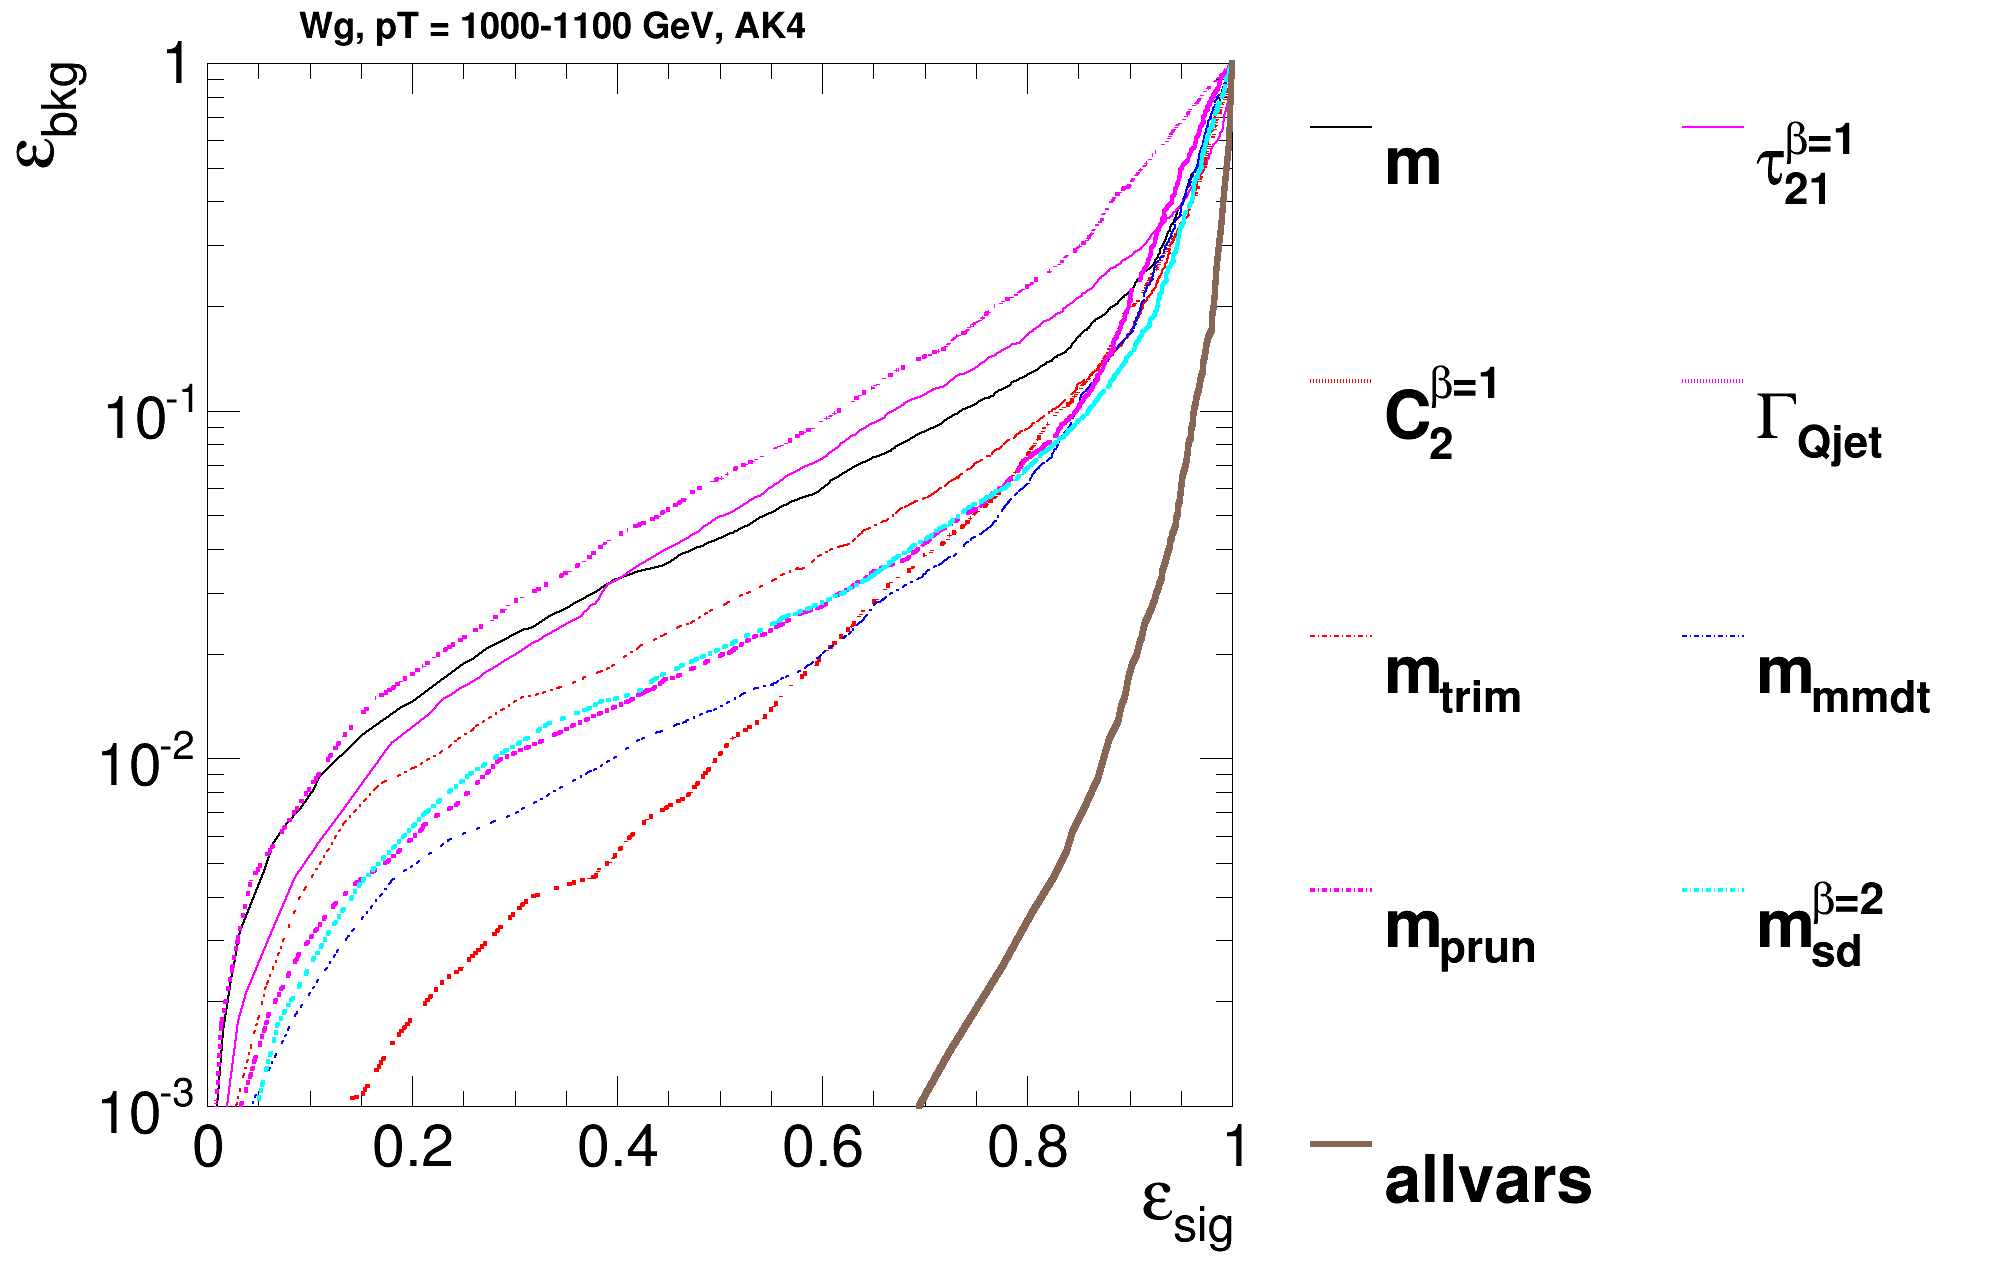
\includegraphics[width=0.7\textwidth]{./Figures/figs072514/figs071614_Wg_bin1000_ak04/rocs/Rocs_1D_single.png}}
\subfigure[\antikt R=0.8, \pt 1.0-1.1 TeV bin]{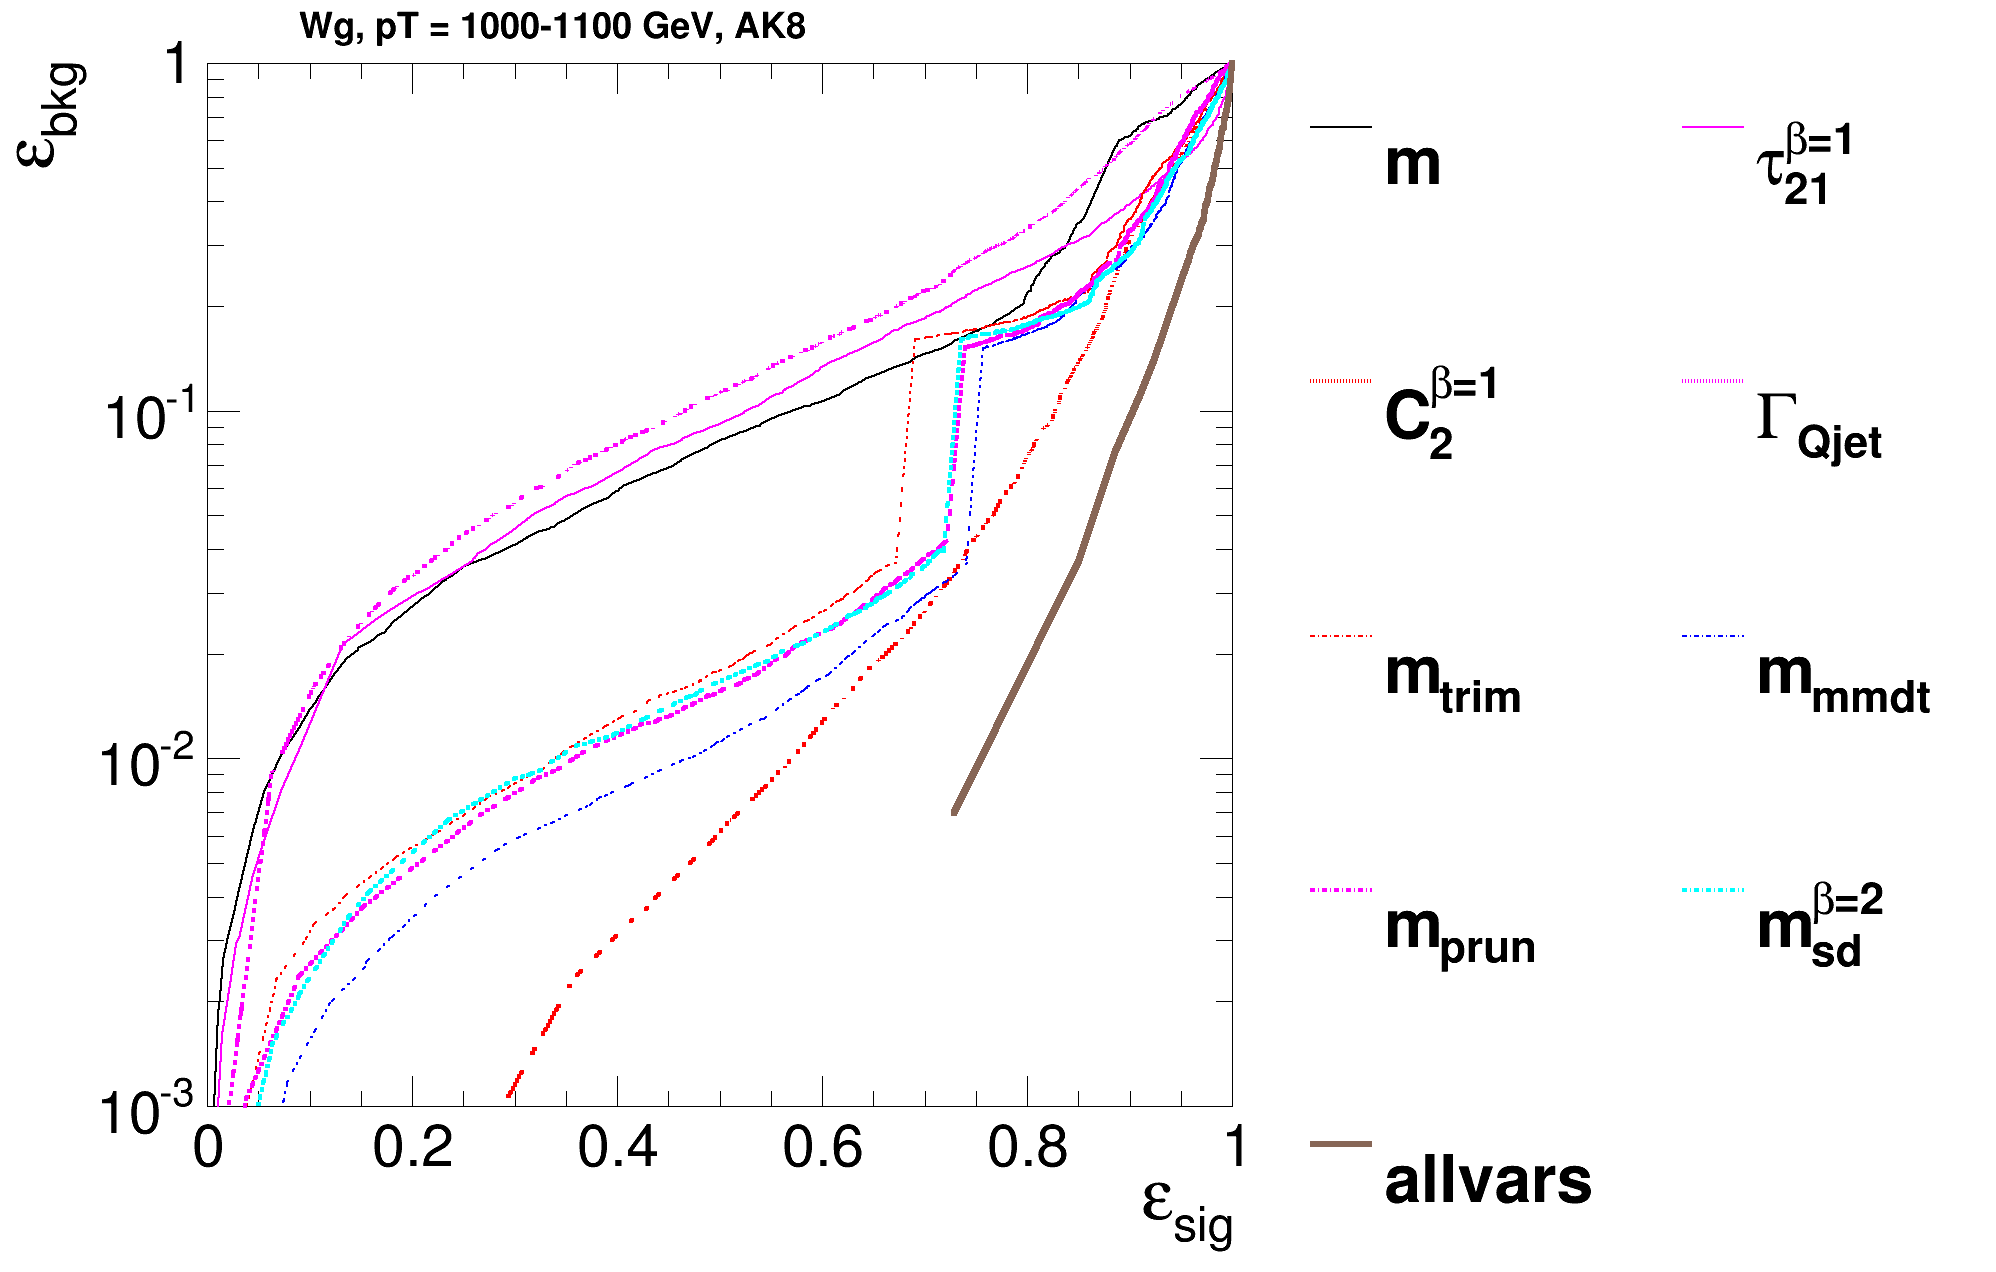
\includegraphics[width=0.7\textwidth]{./Figures/figs072514/figs071614_Wg_bin1000_ak08/rocs/Rocs_1D_single.png}}
\subfigure[\antikt R=1.2, \pt 1.0-1.1 TeV bin]{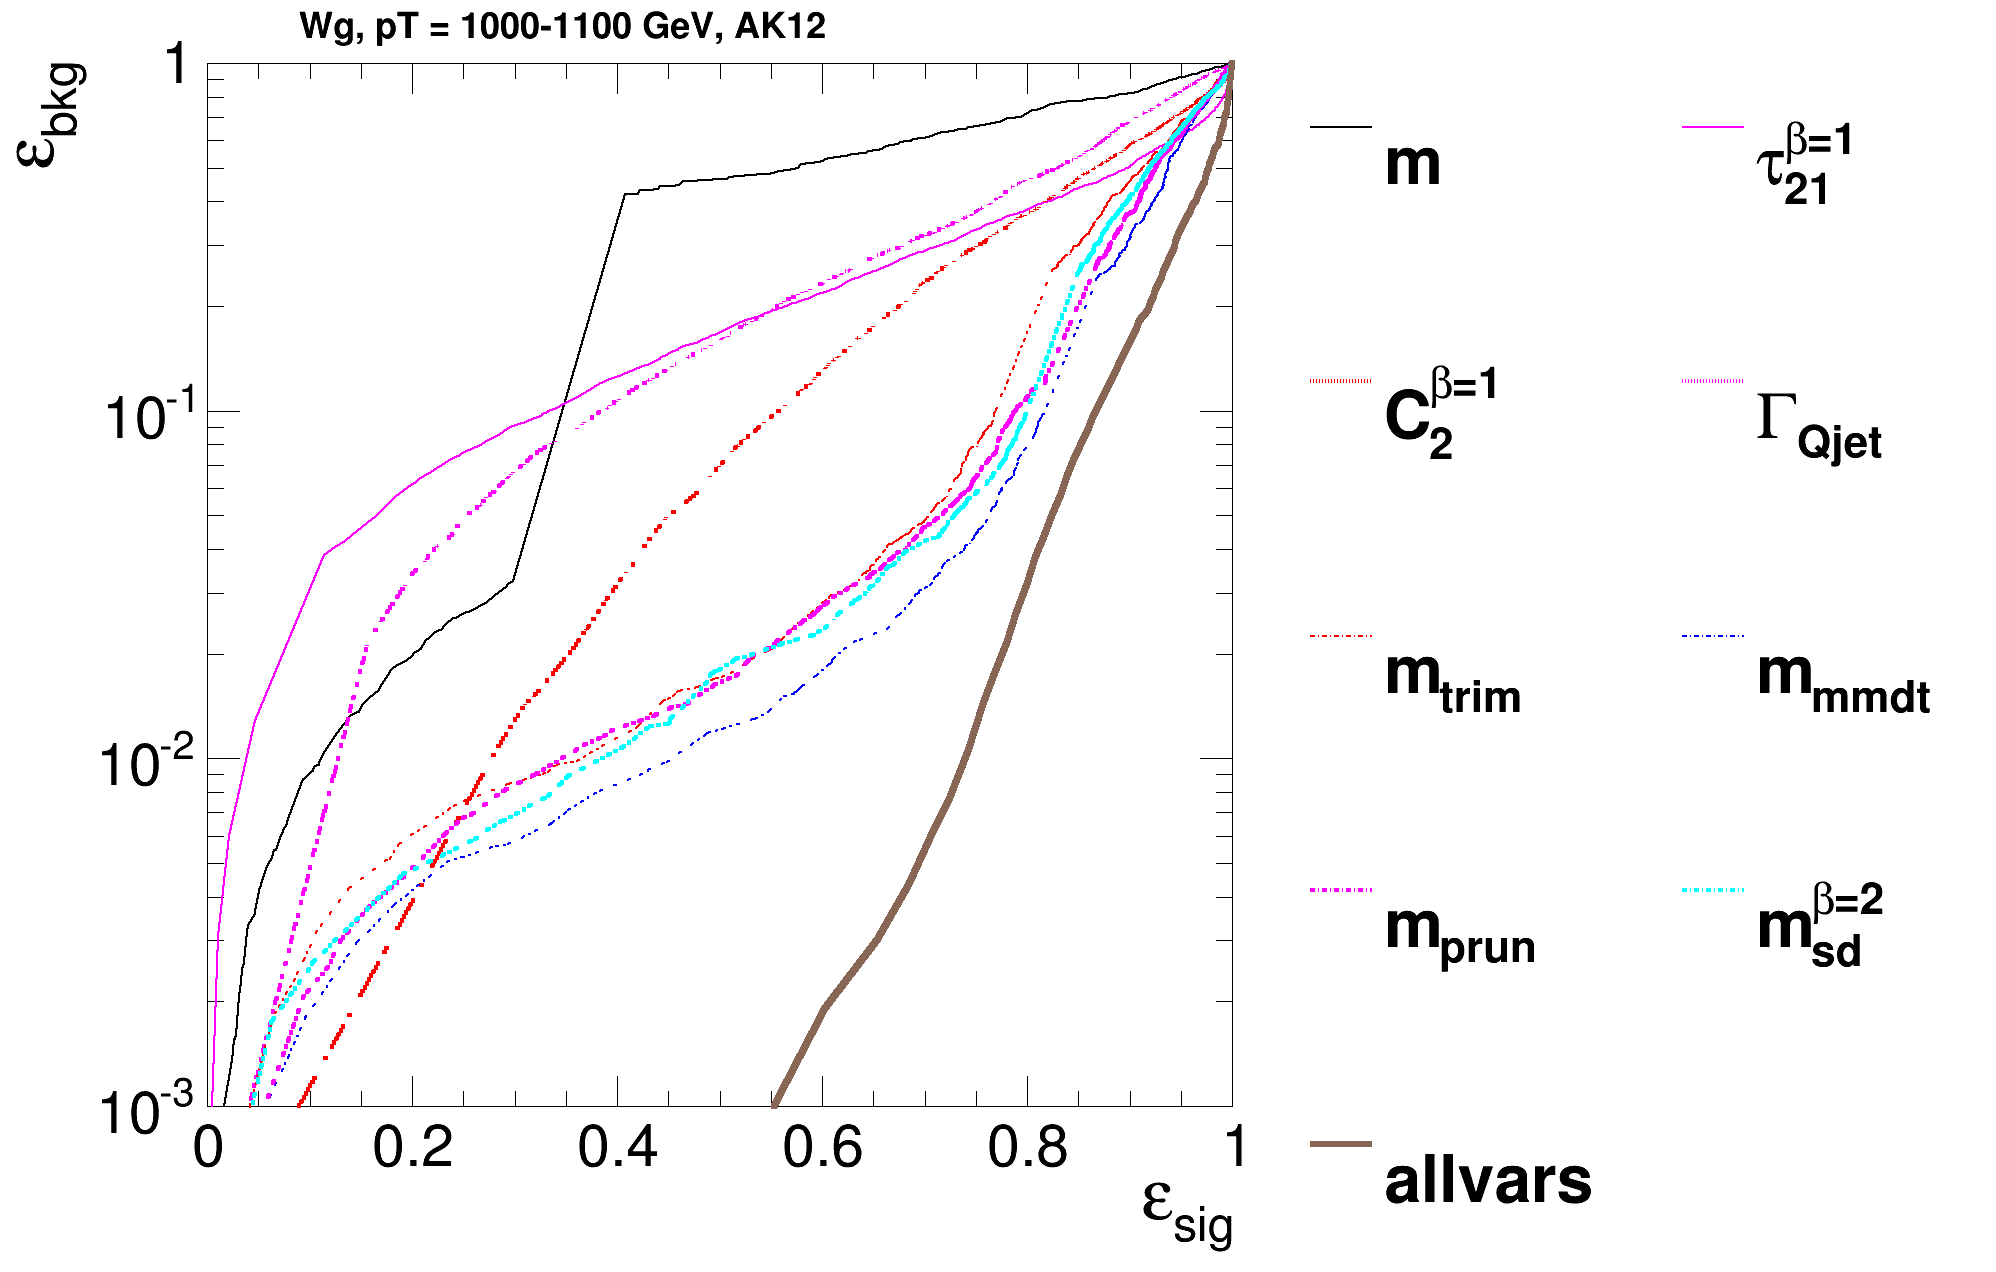
\includegraphics[width=0.7\textwidth]{./Figures/figs072514/figs071614_Wg_bin1000_ak12/rocs/Rocs_1D_single.png}}
\caption{The ROC curve for all single variables considered for $W$
tagging in the \pt 1.0-1.1 TeV bin using the anti-\kT R=0.4 algorithm (top), anti-\kT R=0.8 algorithm
(middle) and R=1.2 algorithm (bottom).}
\label{fig:pt1000_single}
\end{center}
\end{figure*}

%Figure~\ref{fig:pt500_single_AKt_R12} shows the single variable ROC curves in
%the \pT 500 GeV bin for the anti-\kT R=1.2 algorithm, compared to the
%ROC curve for a BDT combination of all the variables. Comparing to
%Figure~\ref{fig:pt500_single_AKt_R08}, one can see that the
%performance of the groomed masses is quite similar. However, the
%performance of the other non-mass substructure variables is markedly
%different, and better in the R=0.8 case.
%
%\begin{figure*}
%\begin{center}
%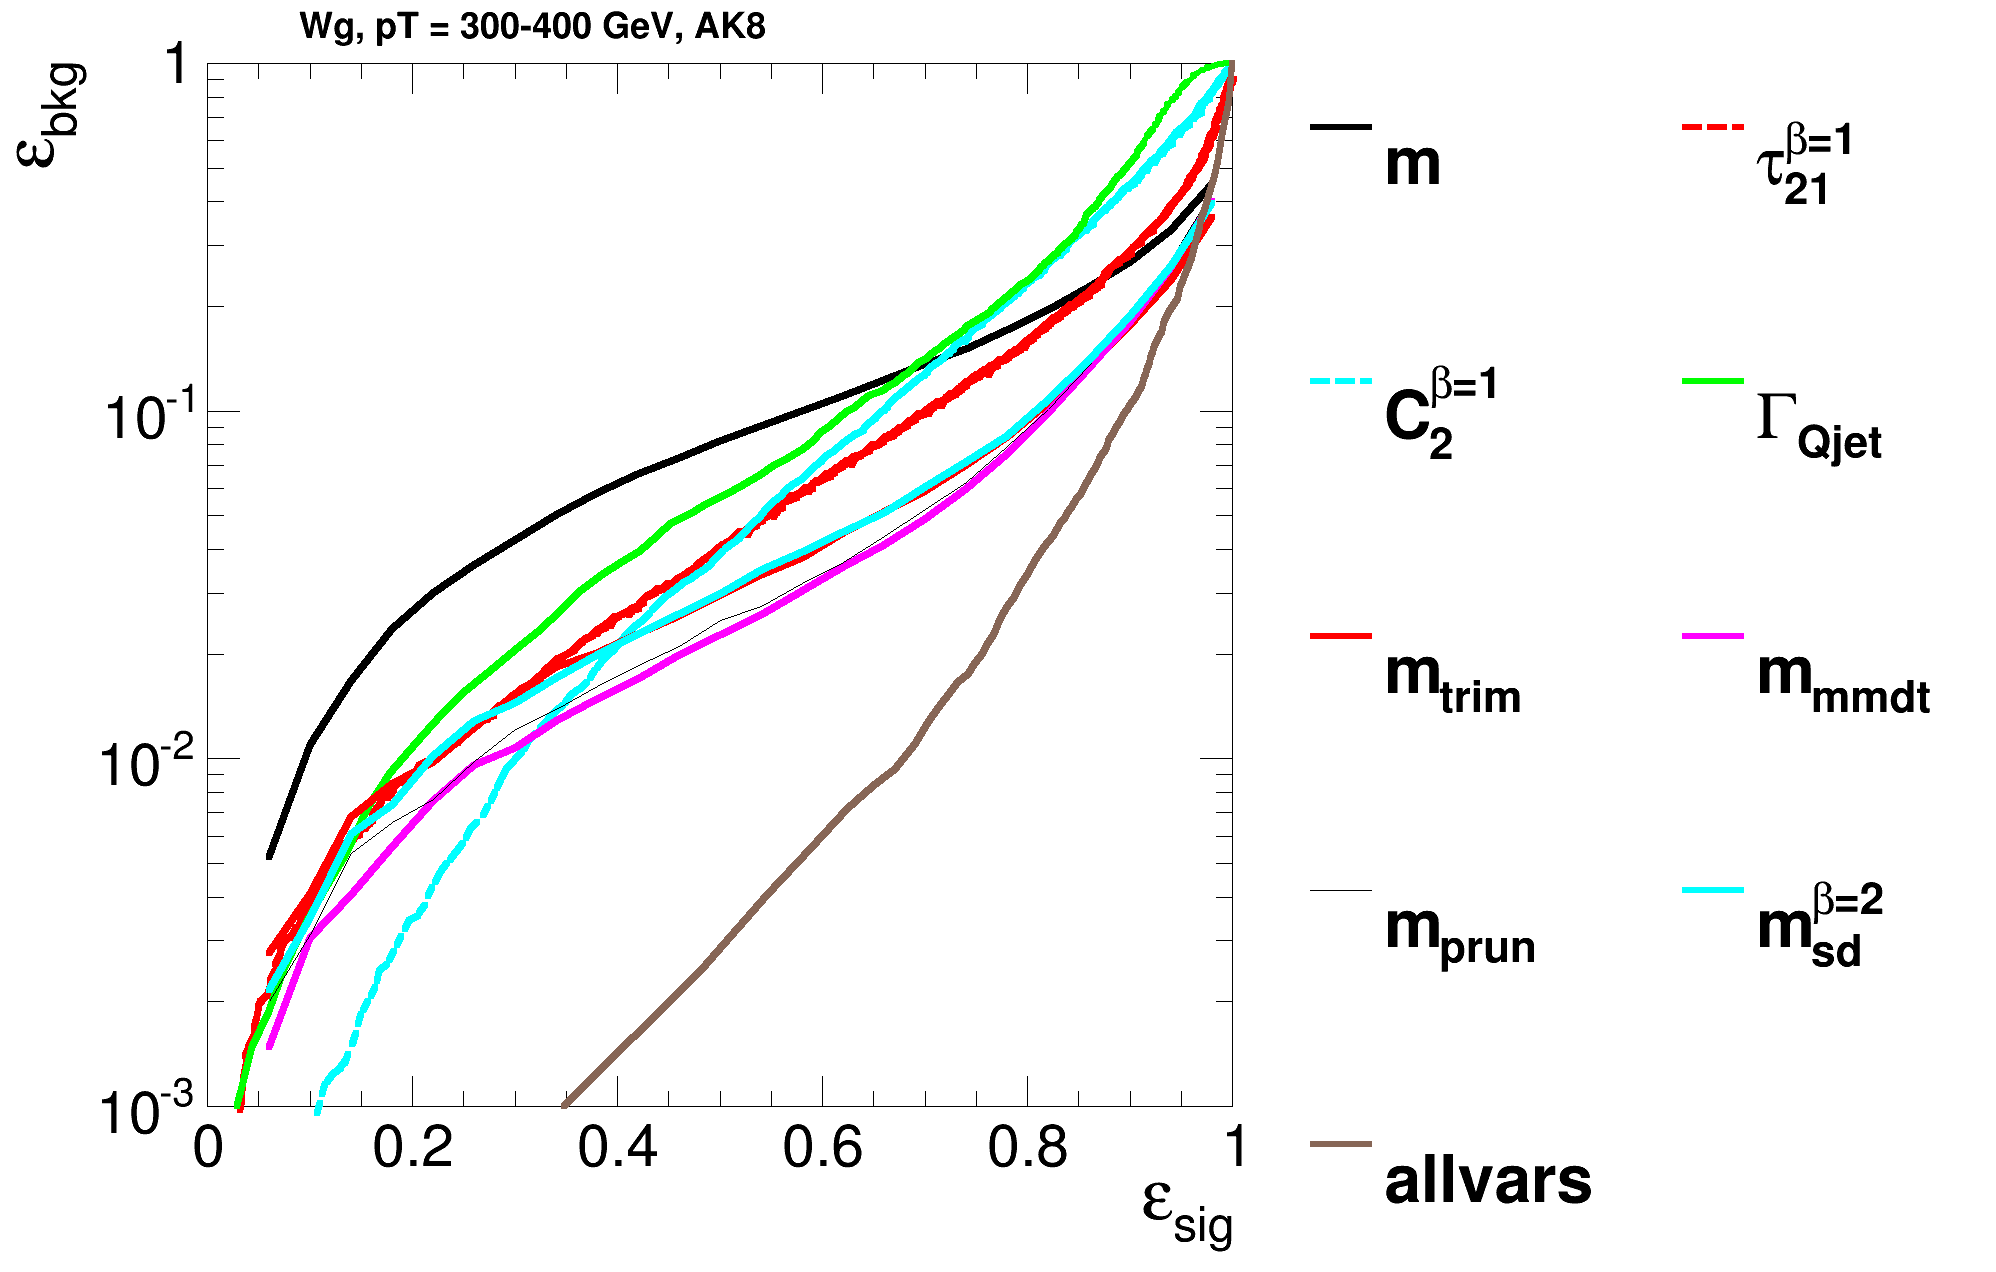
\includegraphics[width=0.8\textwidth]{./Figures/figs072514/figs071614_Wg_bin500_ak12/Rocs_1D_single.png}
%\caption{The ROC curve for all single variables considered for $W$
%tagging in the \pt 500 GeV bin using the anti-\kT R=1.2 algorithm.}
%\label{fig:pt500_single_AKt_R12}
%\end{center}
%\end{figure*}

Although the ROC curves give all the relavant information, it is hard
to compare performance quantitatively. In
Figures~\ref{fig:pt300_comb2D},\ref{fig:pt500_comb2D}
and~\ref{fig:pt1000_comb2D} matrices are shown which give the
background rejection for a signal efficiency of 50\% when two
variables (that on the x-axis and that on the y-axis) are combined in
a BDT. Thus, the diagonal of these plots can be examined to see
quantitatively the individual single variable performance. Because we
have not attempted to optimise the grooming parameter settings of
each grooming algorithm, we do not want to place too much emphasis
here on the relative performance of the groomed masses, but instead
look at the trends veresus \pt and R. One
can see clearly that the background rejection power of the groomed mass
variables increases as the \pt is increased. Within a \pt
bin, one can also see that the groomed mass performance is rather invariant to
changes in the jet radius. In contrast, the substructure variable
performance varies considerably as the jet radius is changed. In
general, the background rejection power of individual jet substructure
variables gets worse as the jet radius is increased. The only
exception to this is in the highest \pt~bin, where the background
rejection power of $C_2^{\beta=1}$ improves when going from jet radius
R=0.4 to R=0.8, but then gets worse again as we go to R=1.2. {\it
  Insert some nice discussion/explanation of why jet substructure
  power generally gets worse as we go to large jet radius, but groomed
mass performance does not}

\begin{figure*}
\begin{center}
\subfigure[\antikt R=0.8, \pt 300-400 GeV bin]{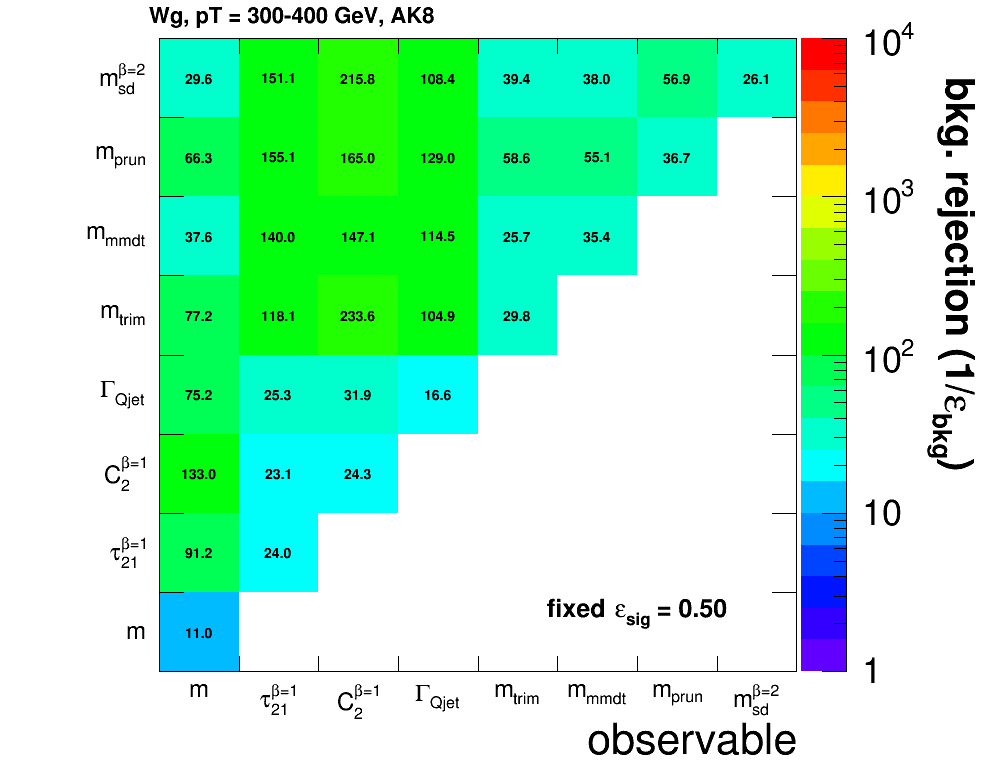
\includegraphics[width=0.5\textwidth]{./Figures/figs072514/figs071614_Wg_bin300_ak08/rocs/effBkg2D.png}}
\subfigure[\antikt R=1.2, \pt 300-400 GeV bin]{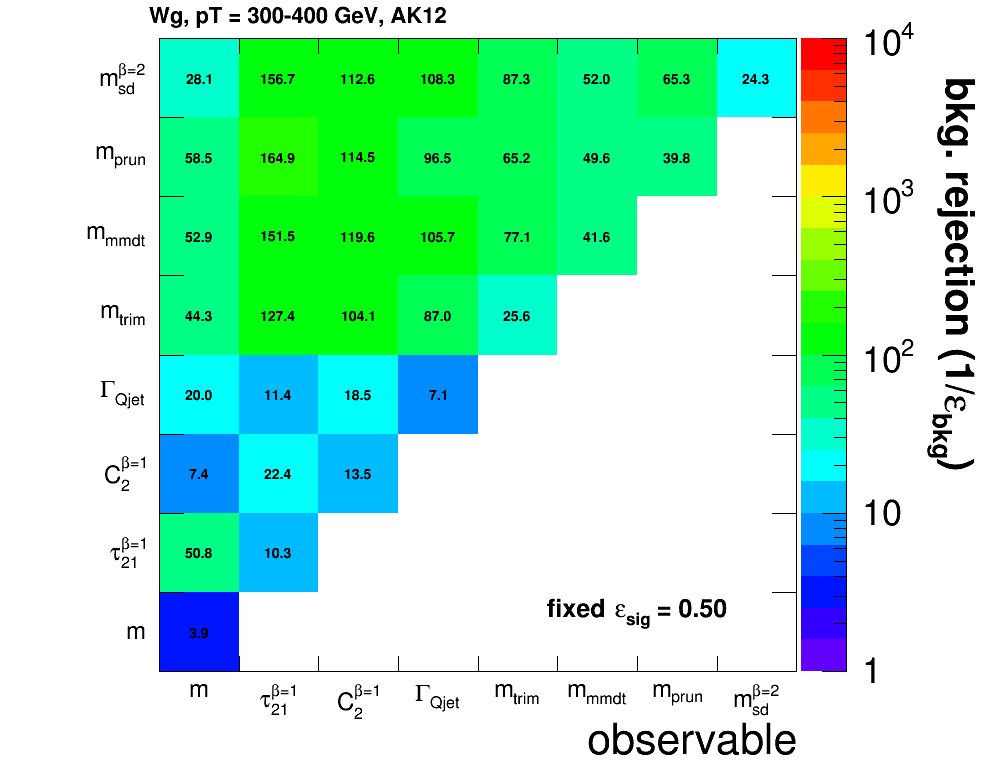
\includegraphics[width=0.5\textwidth]{./Figures/figs072514/figs071614_Wg_bin300_ak12/rocs/effBkg2D.png}}
\caption{
The background rejection
for a fixed signal efficiency (50\%) of each BDT combination of
each pair of variables considered, in the \pt 300-400 GeV bin using the anti-\kT R=0.8
algorithm (top) and R=1.2 algorithm (bottom).
}
\label{fig:pt300_comb2D}
\end{center}
\end{figure*}


\begin{figure*}
\begin{center}
\subfigure[\antikt R=0.8, \pt 500-600 GeV bin]{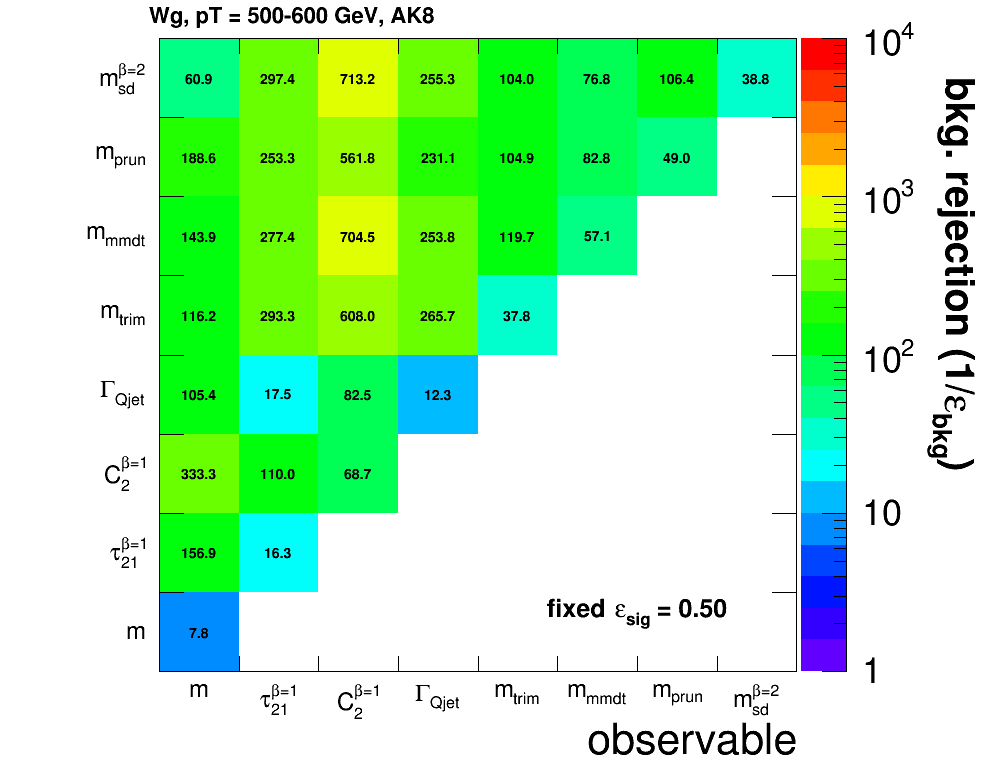
\includegraphics[width=0.5\textwidth]{./Figures/figs072514/figs071614_Wg_bin500_ak08/rocs/effBkg2D.png}}
\subfigure[\antikt R=1.2, \pt 500-600 GeV bin]{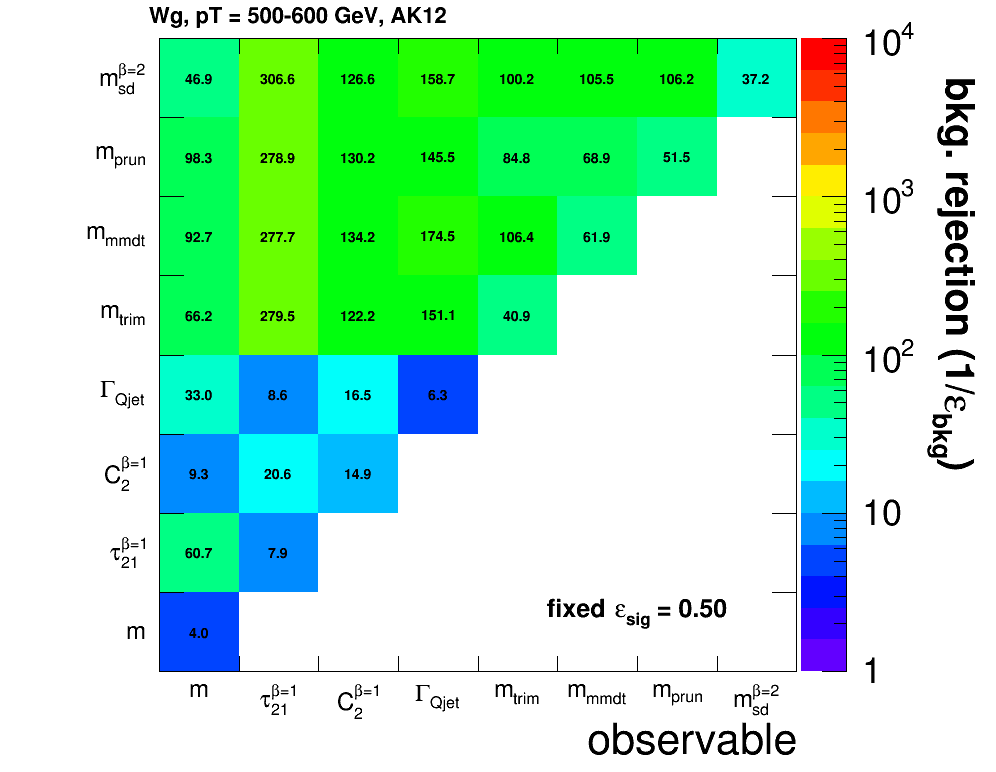
\includegraphics[width=0.5\textwidth]{./Figures/figs072514/figs071614_Wg_bin500_ak12/rocs/effBkg2D.png}}
\caption{The background rejection
for a fixed signal efficiency (50\%) of each BDT combination of
each pair of variables considered, in the \pt 500-600 GeV bin using the anti-\kT R=0.8
algorithm (top) and R=1.2 algorithm (bottom).}
\label{fig:pt500_comb2D}
\end{center}
\end{figure*}

\begin{figure*}
\begin{center}
\subfigure[\antikt R=0.4, \pt 1.0-1.1 TeV bin]{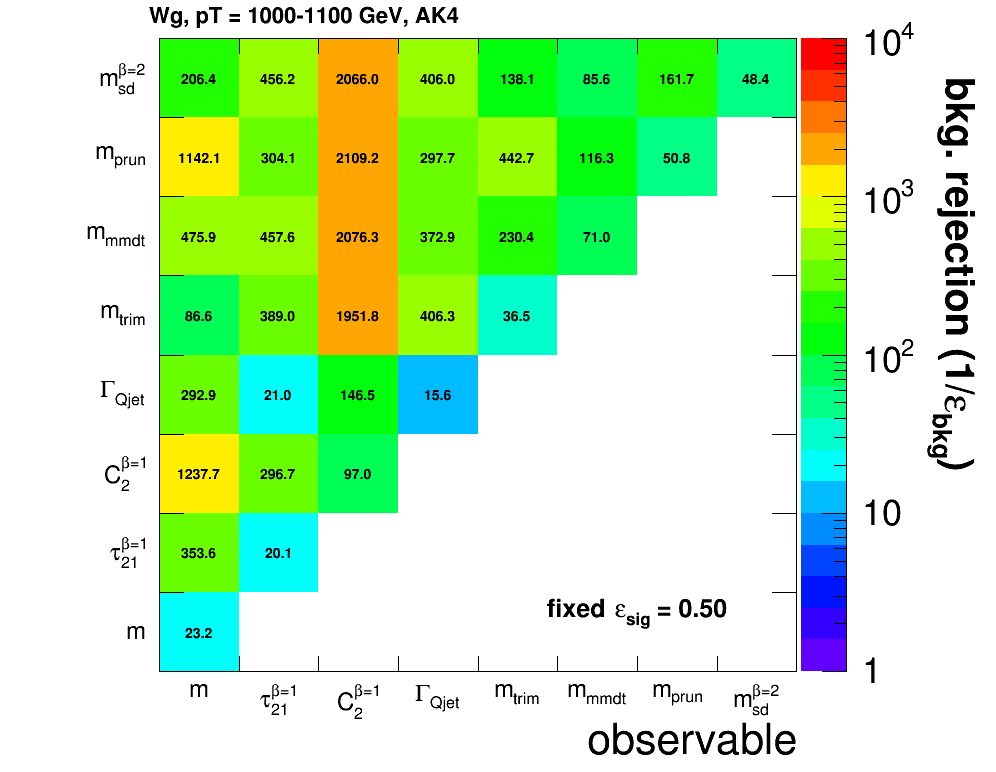
\includegraphics[width=0.5\textwidth]{./Figures/figs072514/figs071614_Wg_bin1000_ak04/rocs/effBkg2D.png}}
\subfigure[\antikt R=0.8, \pt 1.0-1.1 TeV bin]{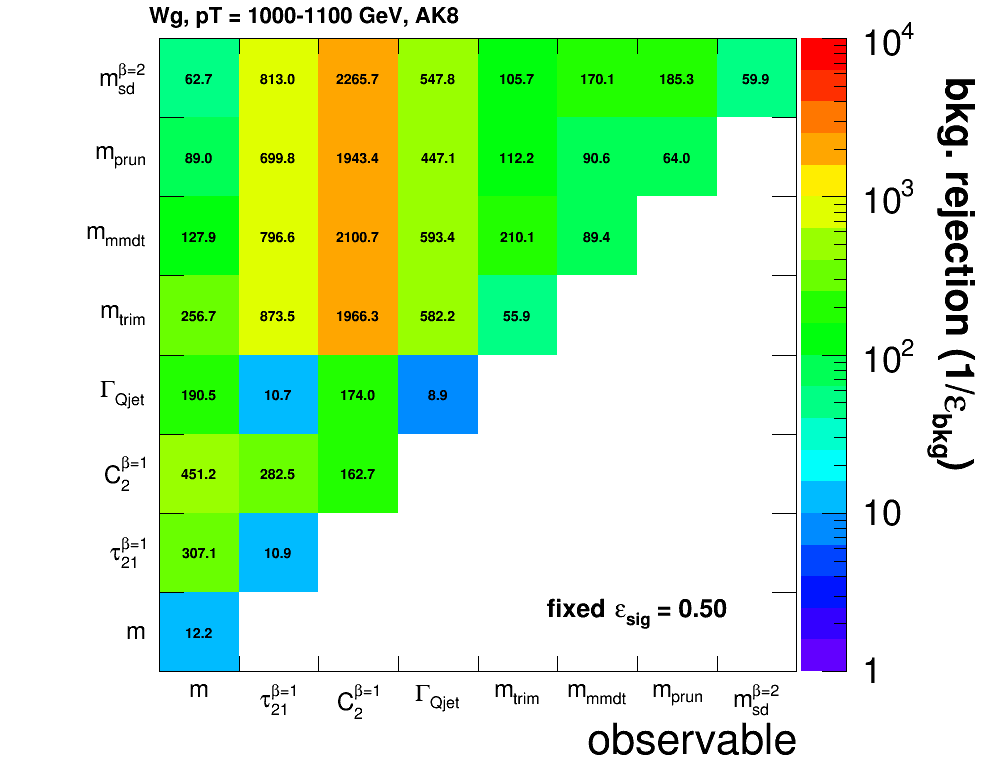
\includegraphics[width=0.5\textwidth]{./Figures/figs072514/figs071614_Wg_bin1000_ak08/rocs/effBkg2D.png}}
\subfigure[\antikt R=1.2, \pt 1.0-1.1 TeV bin]{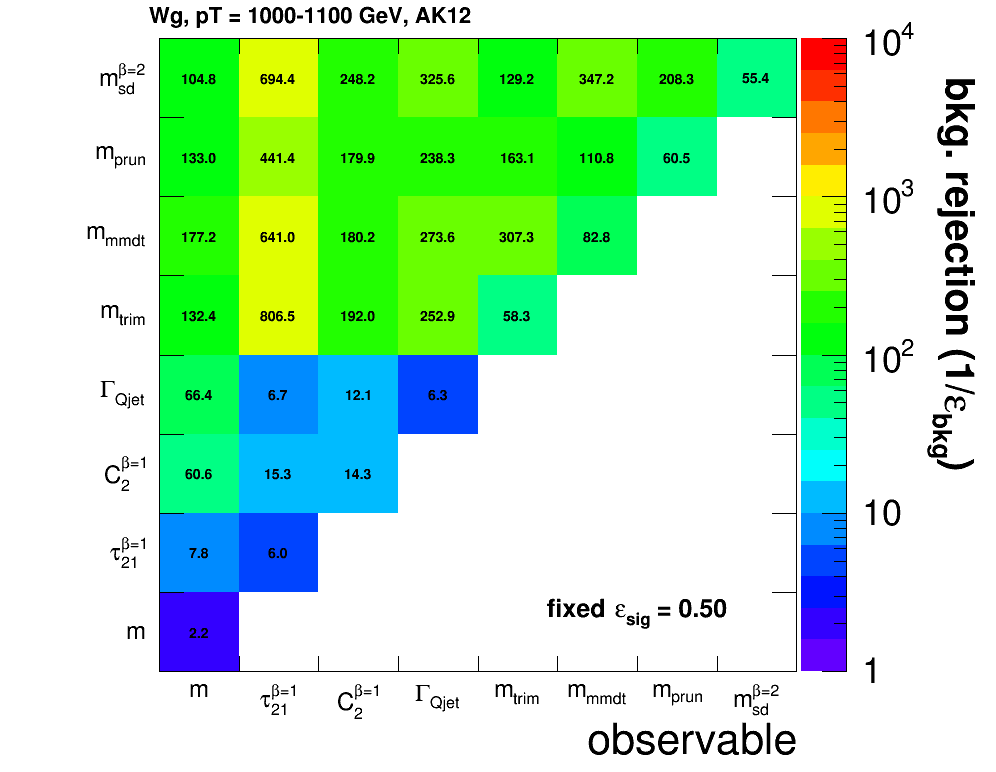
\includegraphics[width=0.5\textwidth]{./Figures/figs072514/figs071614_Wg_bin1000_ak12/rocs/effBkg2D.png}}
\caption{}
\label{fig:pt1000_comb2D}
\end{center}
\end{figure*}


\subsection{Combined Performance}


\subsubsection*{Mass + X Performance}

Figure~\ref{fig:pt500_2Dcomb_AKt_R08} shows the background efficiency
for a fixed signal efficiency (50\%) of each BDT combination of
each pair of variables considered, in the \pt 500 GeV bin using the anti-\kT R=0.8
algorithm. One can see that the best background rejection is achieved
using combinations of the groomed mass variables with other
substructure variables (with the exception
of the soft drop mass with $\beta=-1$). Combinations of the mass
variables themselves are not particularly powerful, but are
interesting for understanding the correlations between the masses (see
Section~\ref{sec:wtag_massplusmass}). Equally, combination of the
substructure variables, without using a mass, are not powerful. 

Figure~\ref{fig:pt500_masscomb_AKt_R08} shows the actual ROC curves of the BDT combinations of each mass variable with every other
variable considered in the \pt 500 GeV bin using the anti-\kT R=0.8
algorithm. {\it Can we drop the combinations of mass + mass
from these plots to make them clearer? Also would be good to put the
single variable mass curve on these plots, so you can see how much
improvement the combination gives, and the ``all variables'' curve.}

No combination with other variables can recover the poor performance
of the ungroomed mass and the soft drop mass with
$\beta=-1$. Figures~\ref{fig:pt500_2Dcomb_AKt_R08}
and~\ref{fig:pt500_masscomb_AKt_R08} show that the
other groomed/filtered masses are all most improved by combination
with the $C_{2}^{\beta=1}$ energy correlation
function. Figure~\ref{fig:pt500_2d_mmdt_AKt_R08} shows the 2-D
correlation plots between the mMDT mass and the $C_{2}^{\beta=1}$,
$\Gamma_{Qjet}$ and $\tau_{21}^{\beta=1}$ variables. One can clearly
see that there is substantially less correlation between the mass and
$C_{2}^{\beta=1}$ than the other variables. Similar results are seen
for the other groomed masses.

\begin{figure*}
\begin{center}
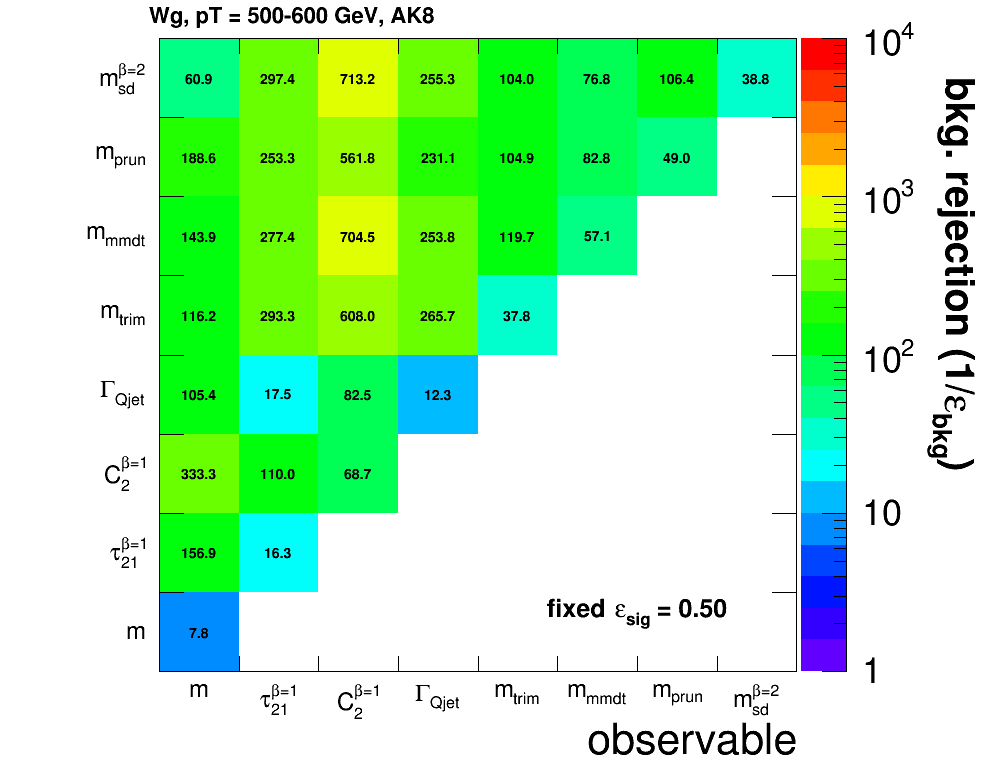
\includegraphics[width=0.48\textwidth]{./Figures/figs072514/figs071614_Wg_bin500_ak08/rocs/effBkg2D.png}
\caption{The background efficiency
for a fixed signal efficiency (50\%) of each BDT combination of
each pair of variables considered, in the \pt 500 GeV bin using the anti-\kT R=0.8
algorithm.}
\label{fig:pt500_2Dcomb_AKt_R08}
\end{center}
\end{figure*}


\begin{figure*}
\begin{center}
\subfigure[Ungroomed mass + X]{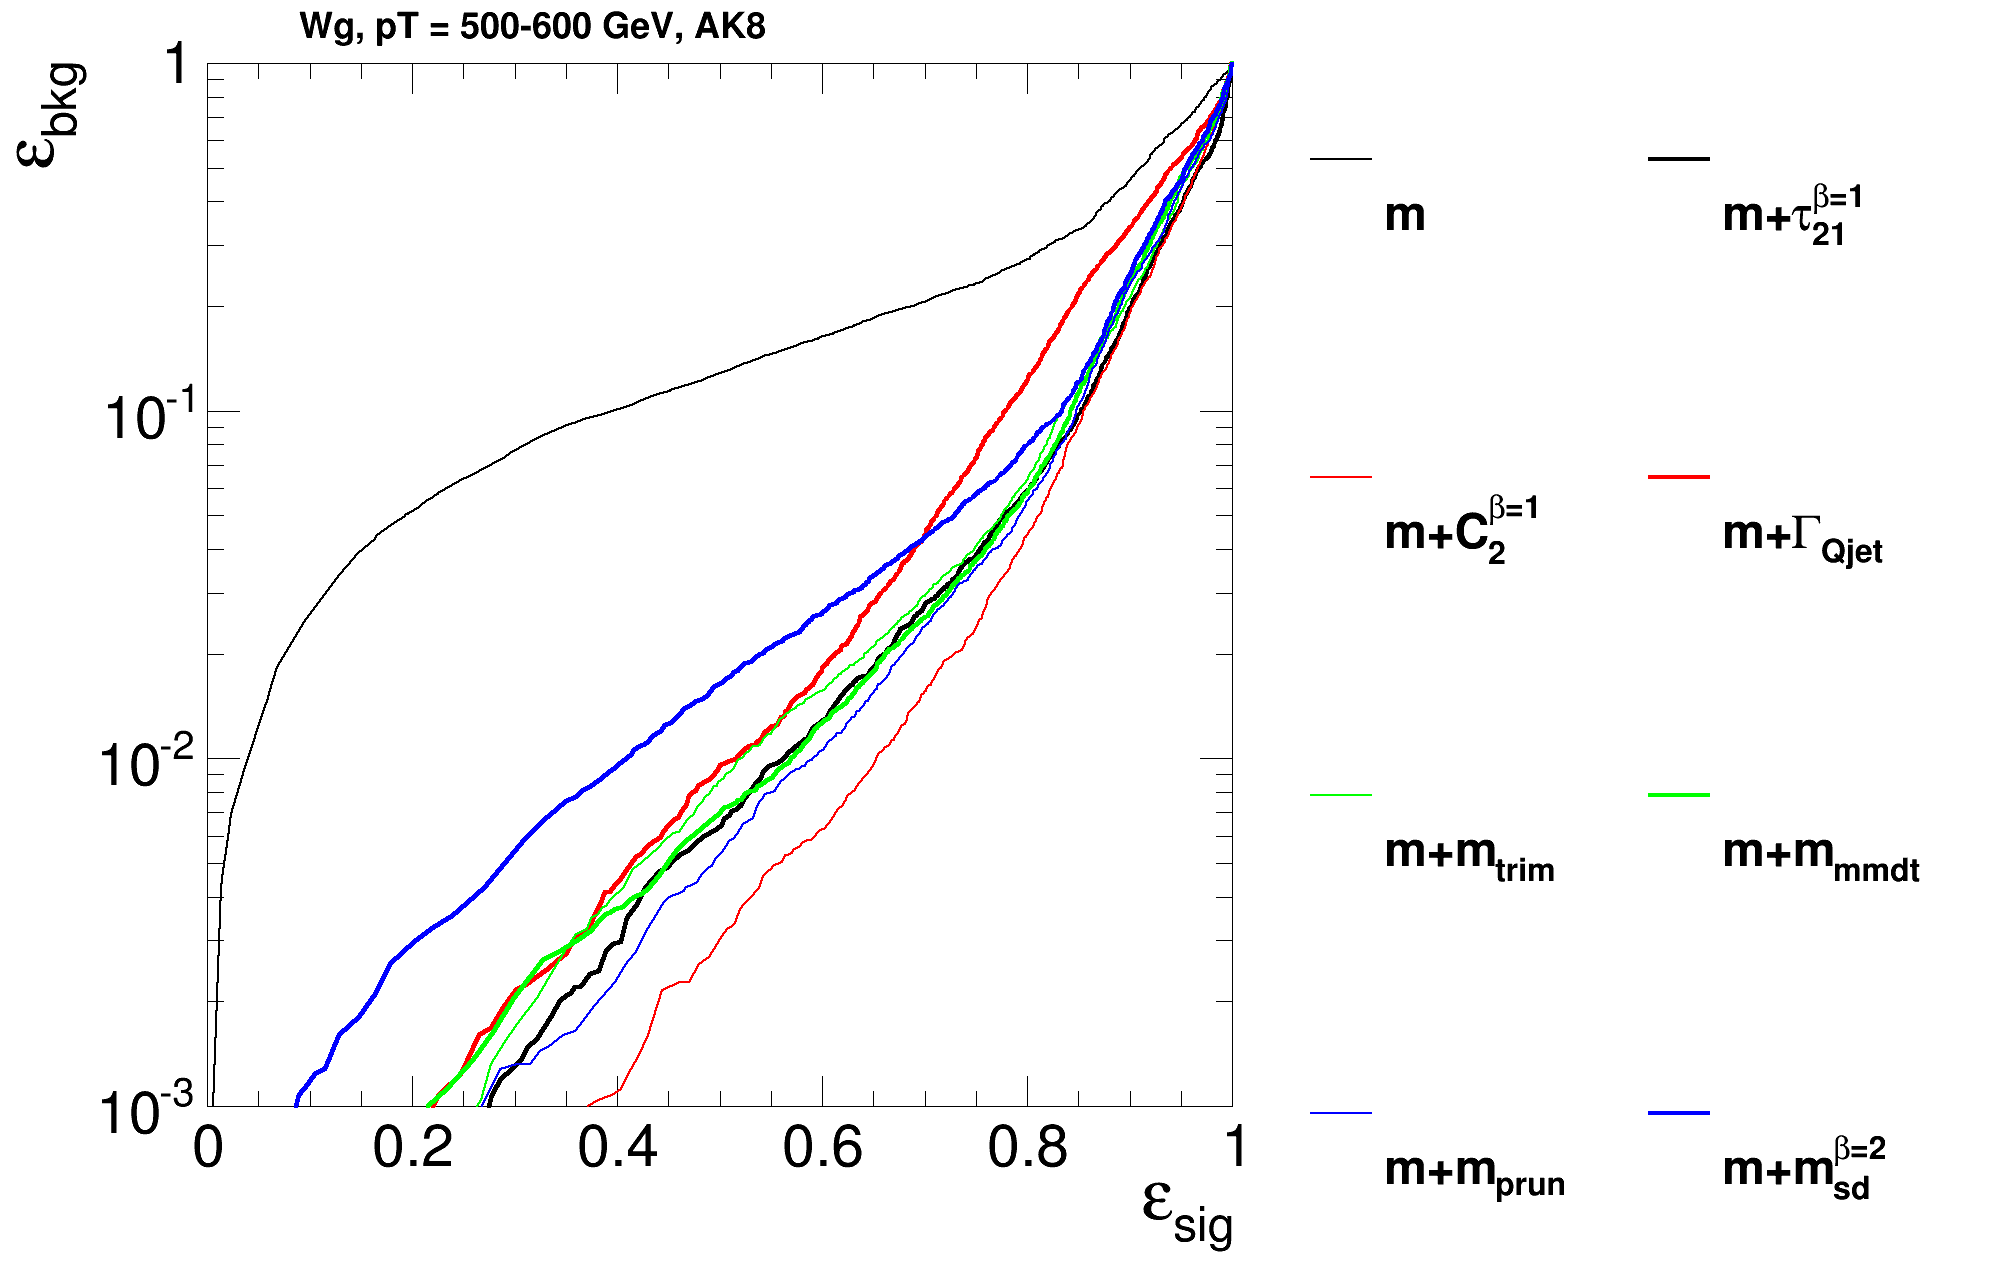
\includegraphics[width=0.48\textwidth]{./Figures/figs072514/figs071614_Wg_bin500_ak08/rocs/Rocs_1D_jmass.png}}
\subfigure[Trimmed mass + X]{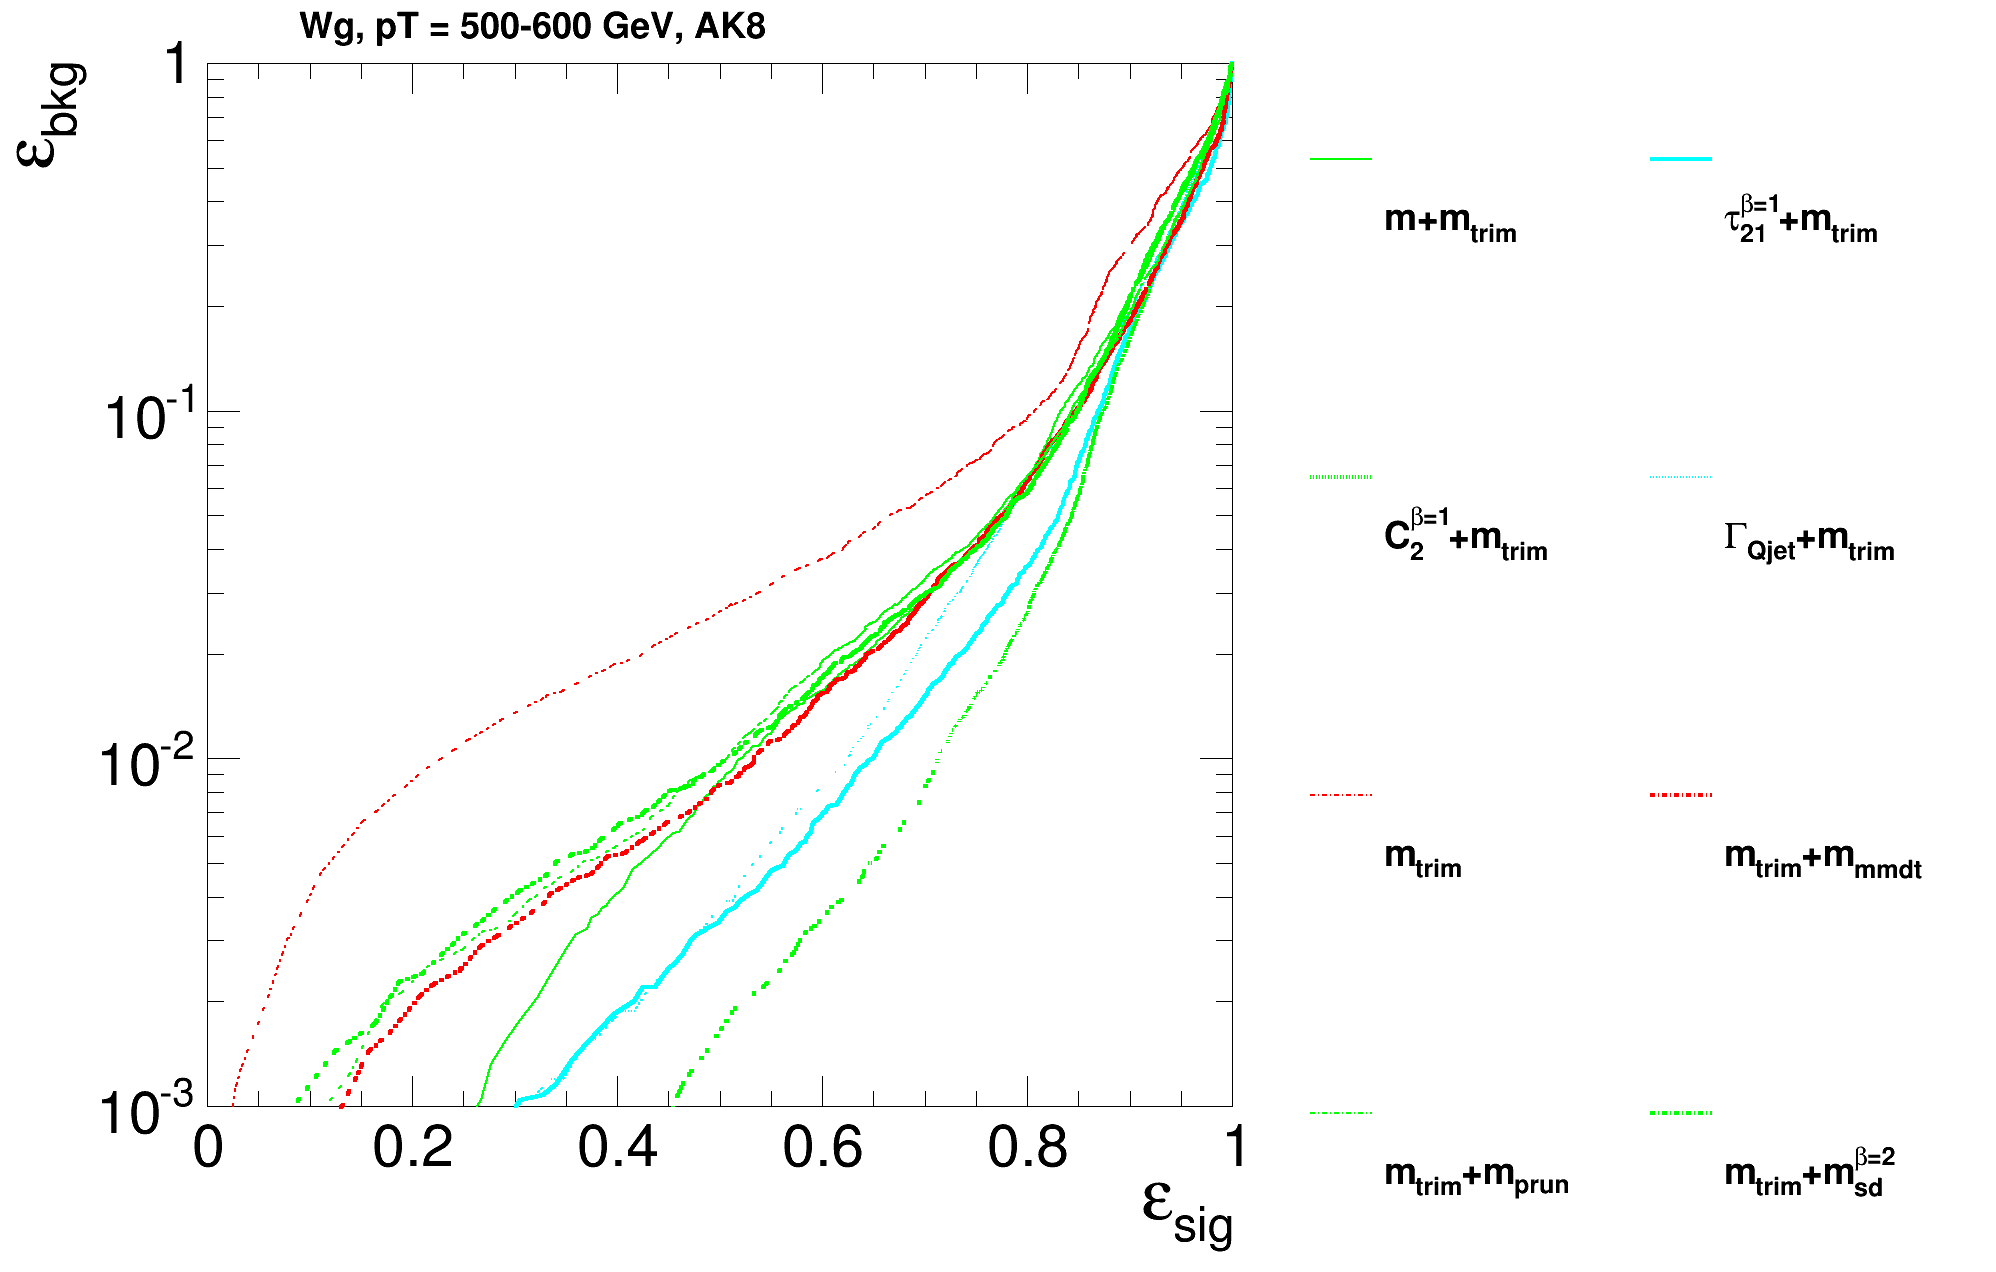
\includegraphics[width=0.48\textwidth]{./Figures/figs072514/figs071614_Wg_bin500_ak08/rocs/Rocs_1D_j_mass_trim.png}}
\subfigure[Pruned mass + X]{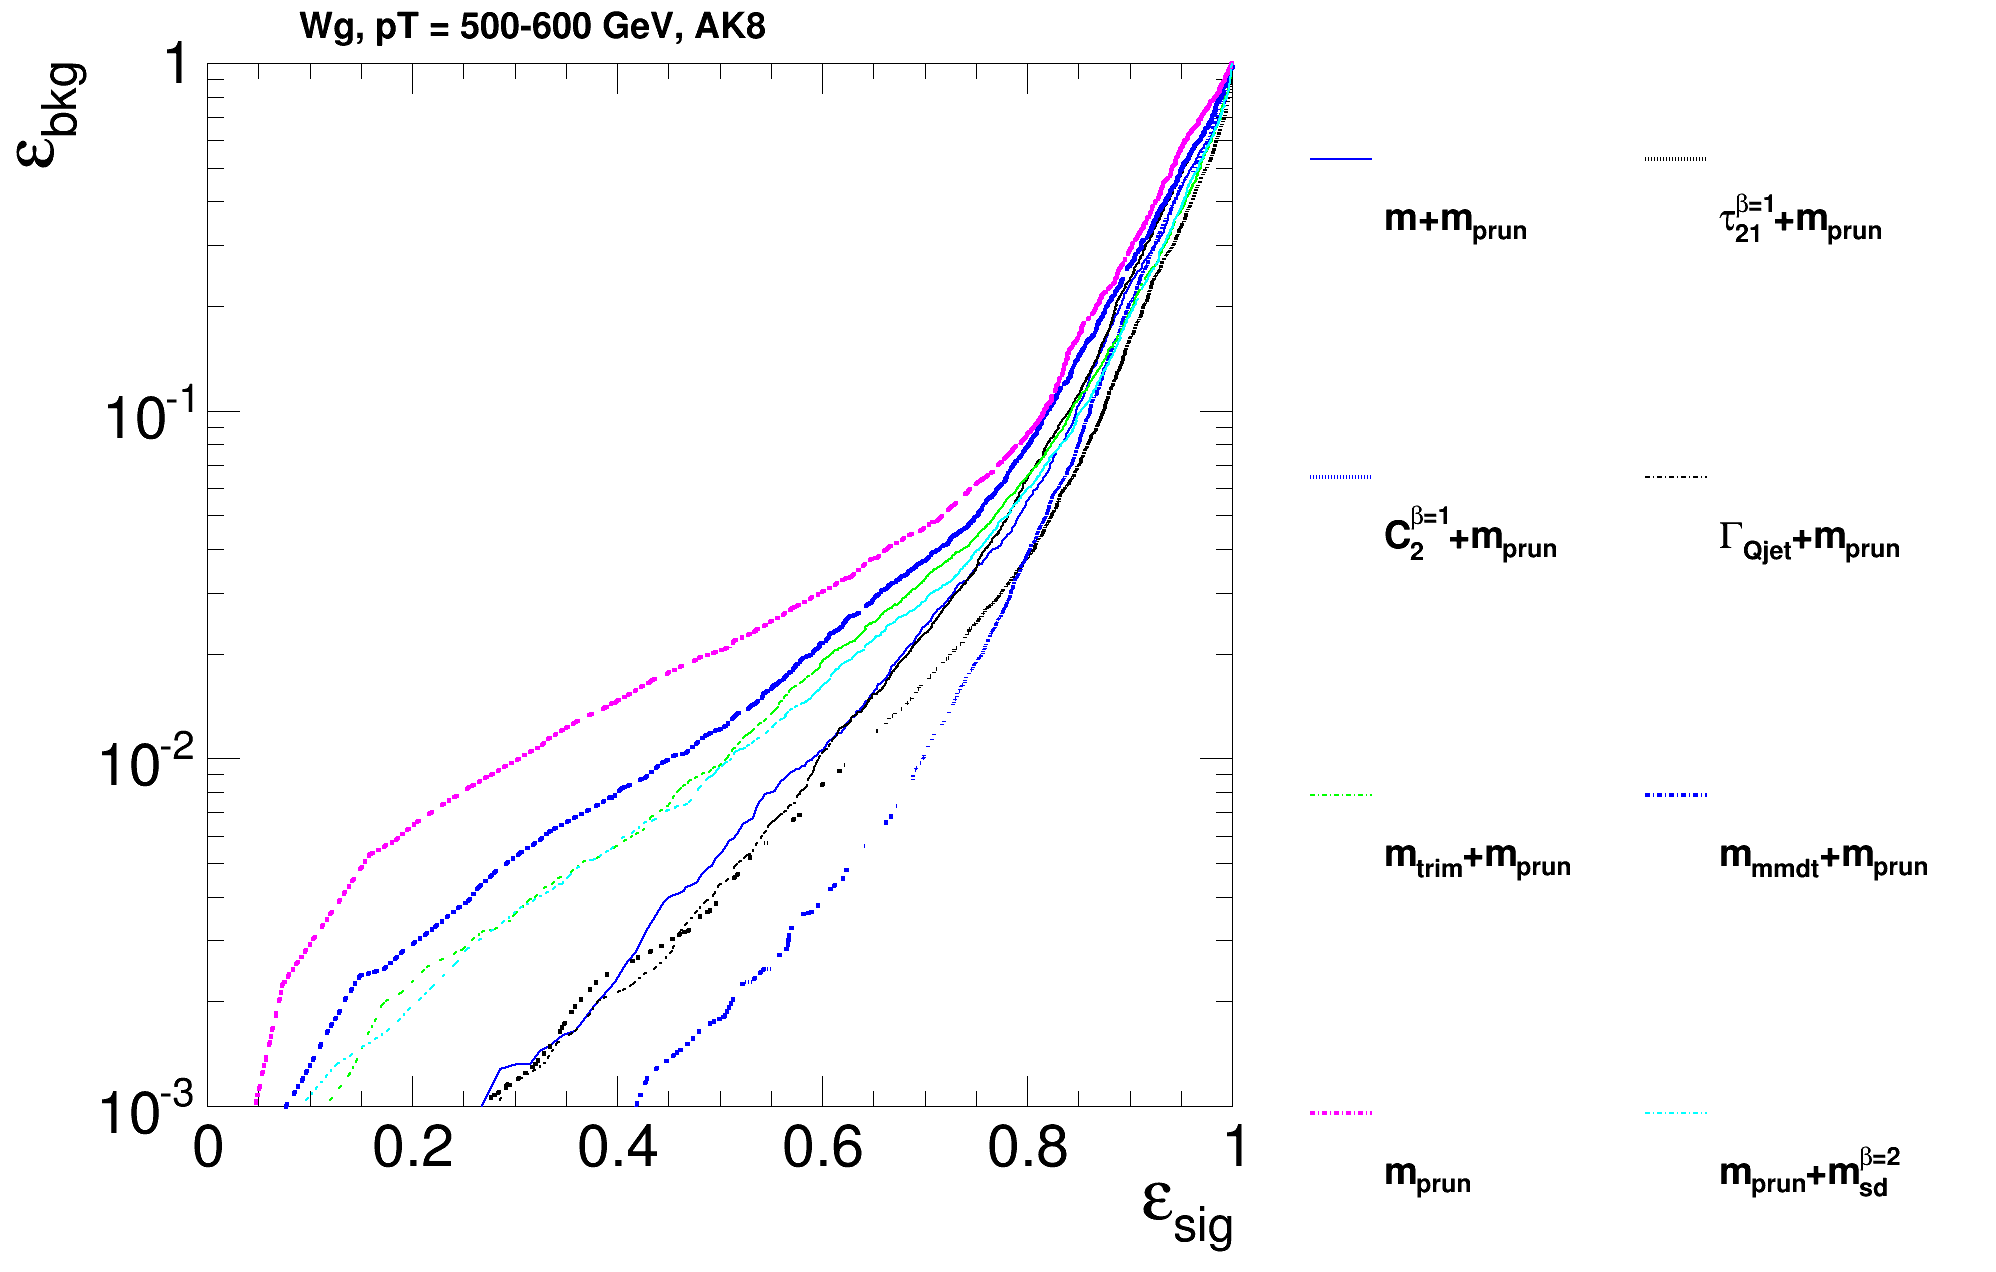
\includegraphics[width=0.48\textwidth]{./Figures/figs072514/figs071614_Wg_bin500_ak08/rocs/Rocs_1D_j_mass_prun.png}}
%\subfigure[Soft drop mass ($\beta=-1$) +X]{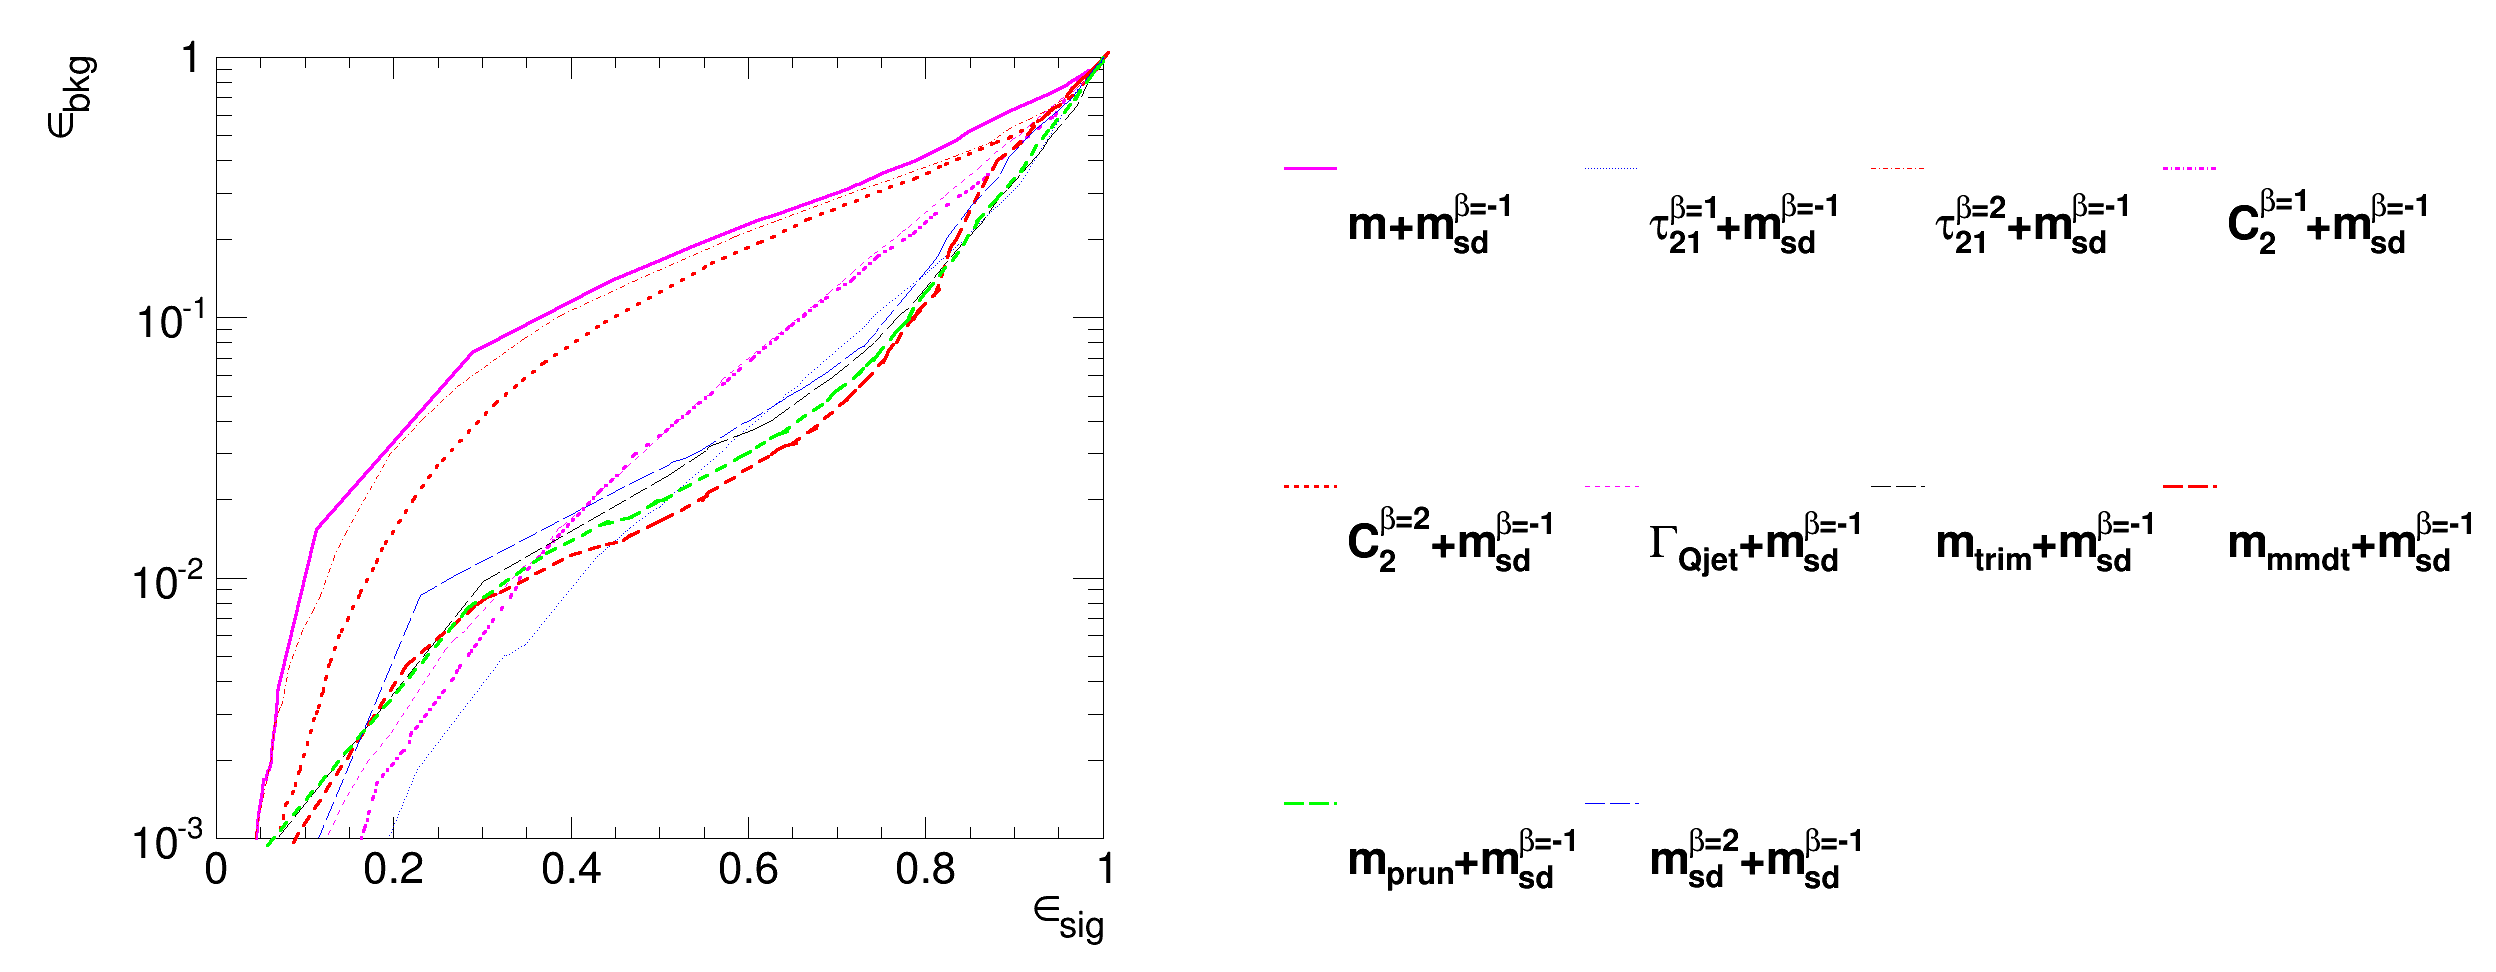
\includegraphics[width=0.48\textwidth]{./Figures/figs072514/figs071614_Wg_bin500_ak08/rocs/Rocs_1D_j_mass_sdm1.png}}
\subfigure[Soft drop mass ($\beta=2$) + X]{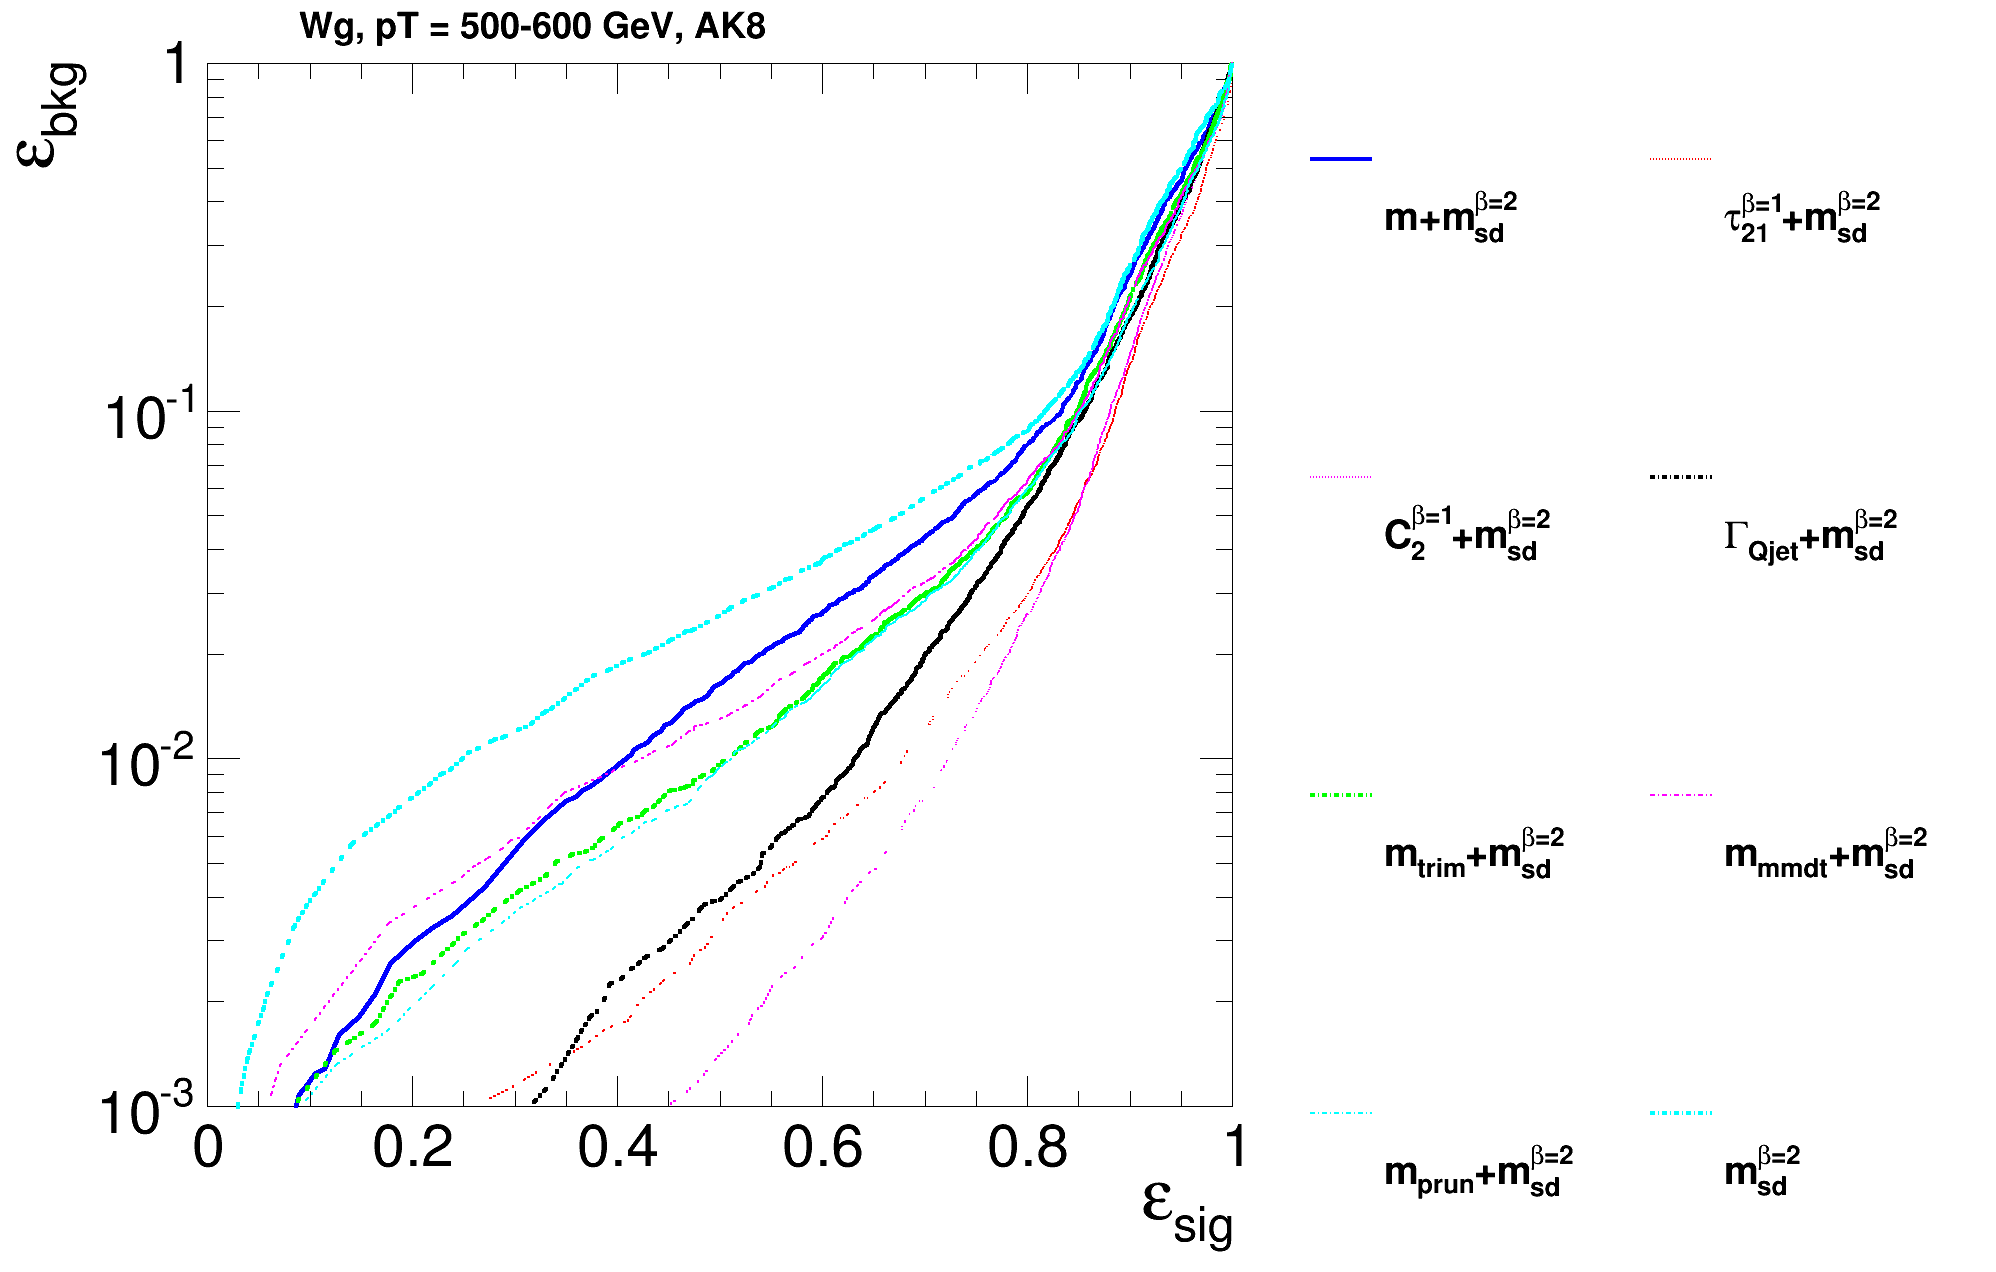
\includegraphics[width=0.48\textwidth]{./Figures/figs072514/figs071614_Wg_bin500_ak08/rocs/Rocs_1D_j_mass_sdb2.png}}
\subfigure[mMDT mass + X]{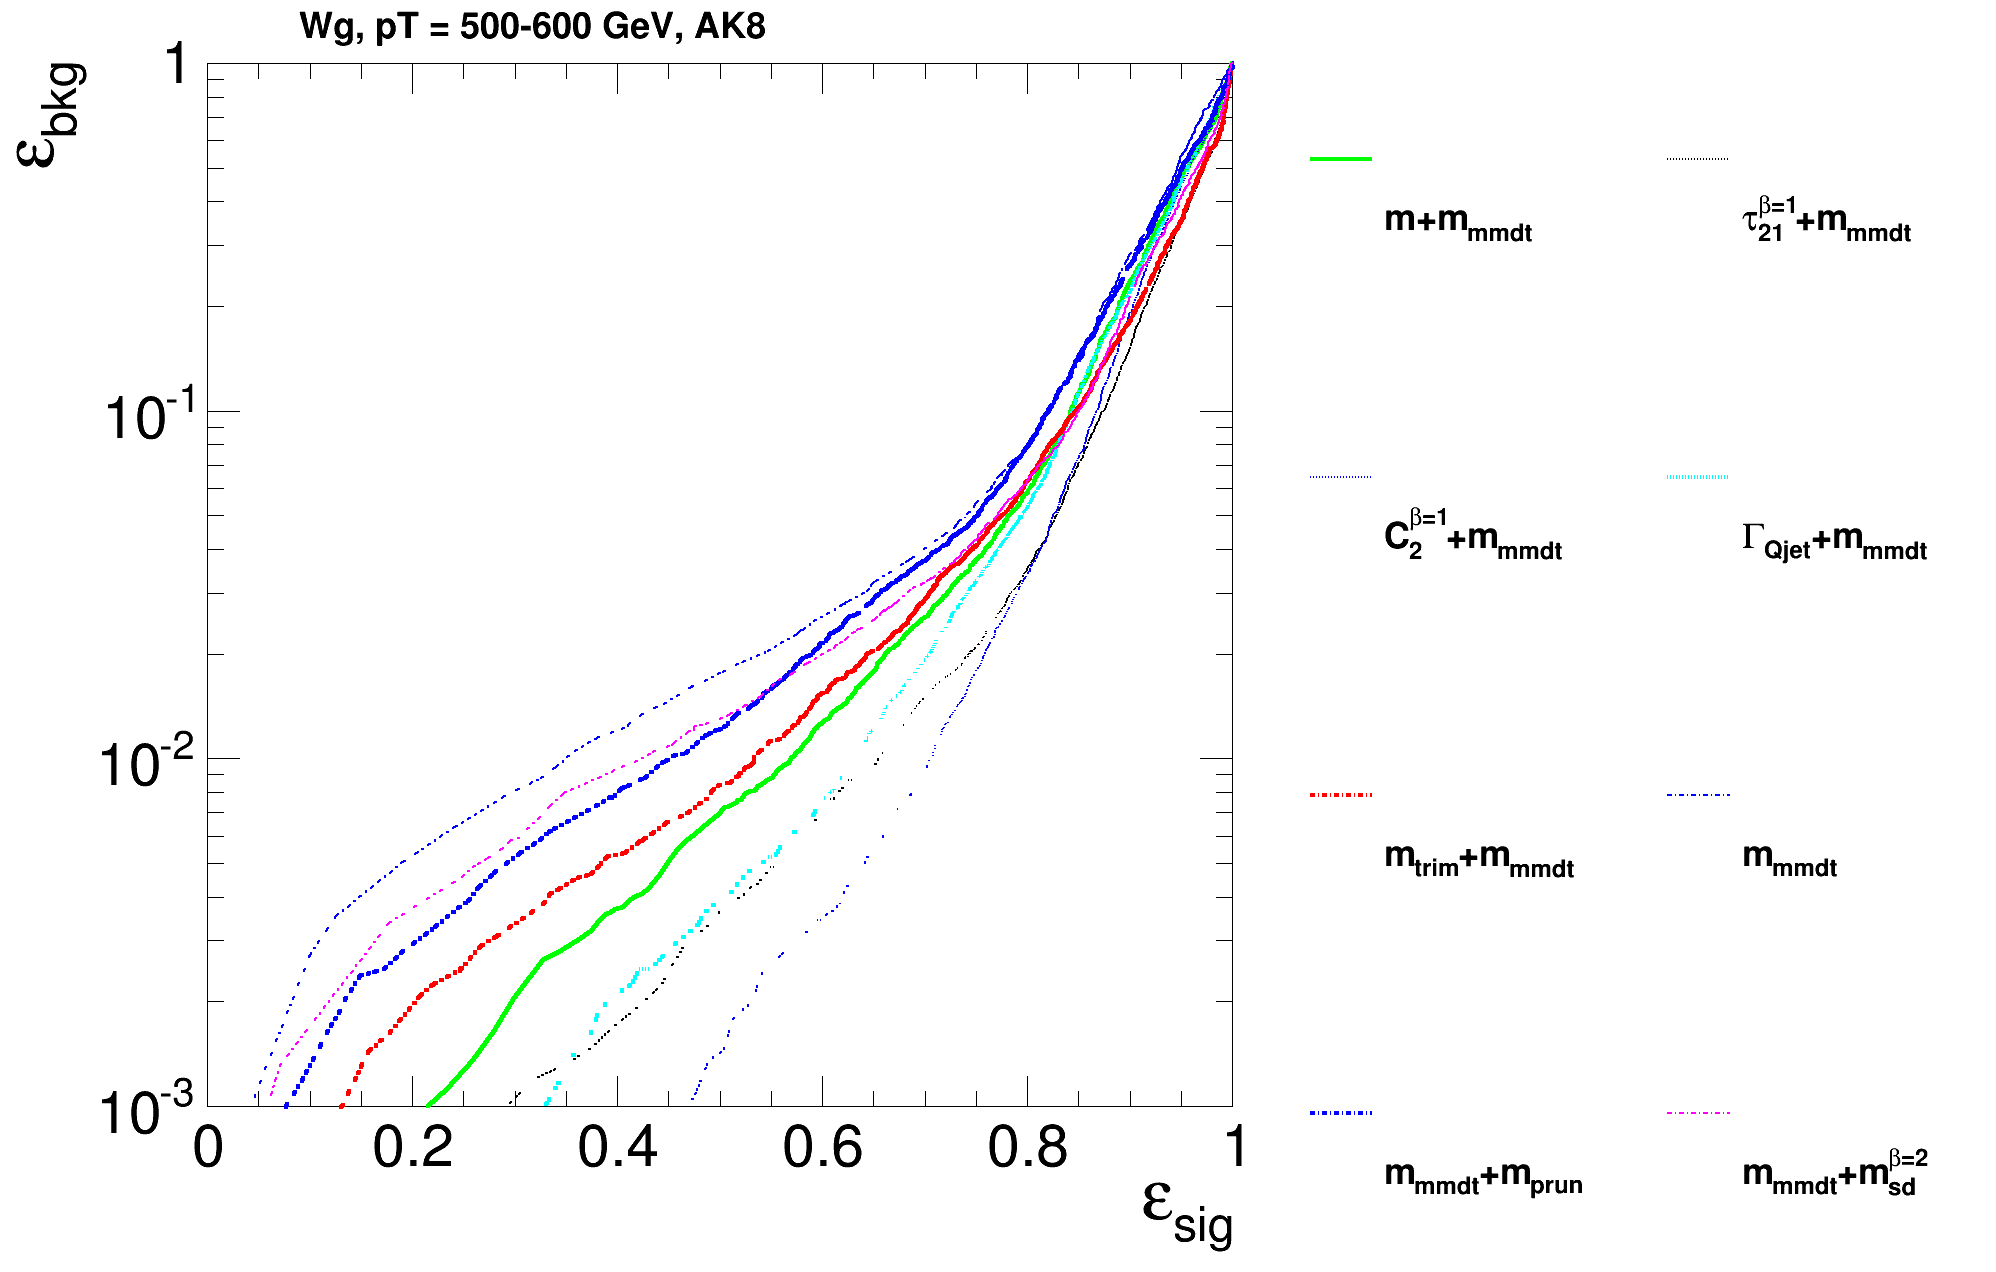
\includegraphics[width=0.48\textwidth]{./Figures/figs072514/figs071614_Wg_bin500_ak08/rocs/Rocs_1D_j_mass_mmdt.png}}
\caption{The BDT combinations of each mass variable with every other
variable considered in the \pt 500 GeV bin using the anti-\kT R=0.8 algorithm.}
\label{fig:pt500_masscomb_AKt_R08}
\end{center}
\end{figure*}


\begin{figure*}
\begin{center}
\subfigure[mMDT mass vs $C_2^{\beta=1}$]{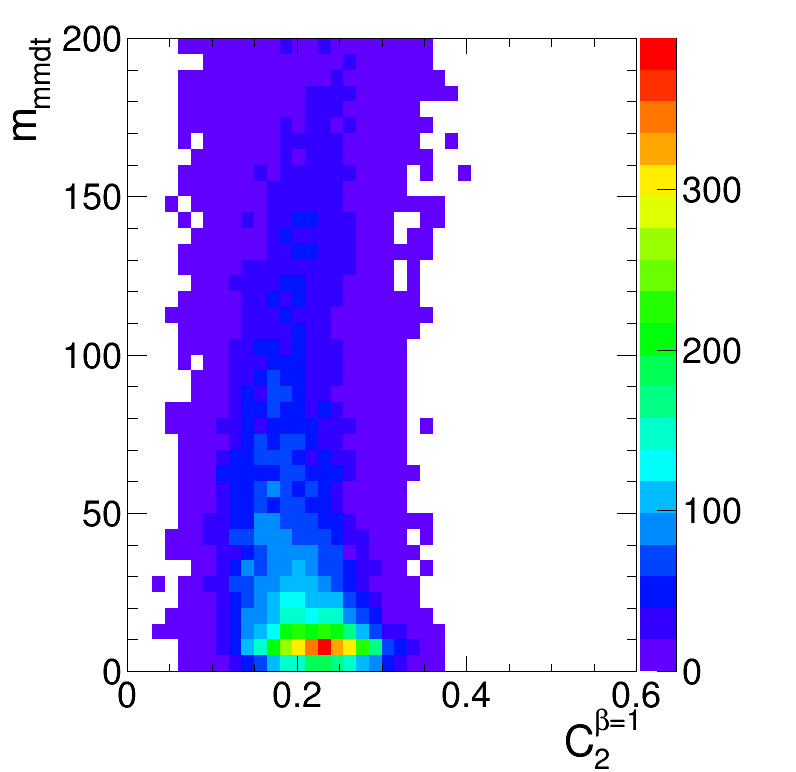
\includegraphics[width=0.48\textwidth]{./Figures/figs072514/figs071614_Wg_bin500_ak08/twoD/h2d_jc2_b1_j_mass_mmdt_gg.png}}
\subfigure[mMDT mass vs $\Gamma_{Qjet}$]{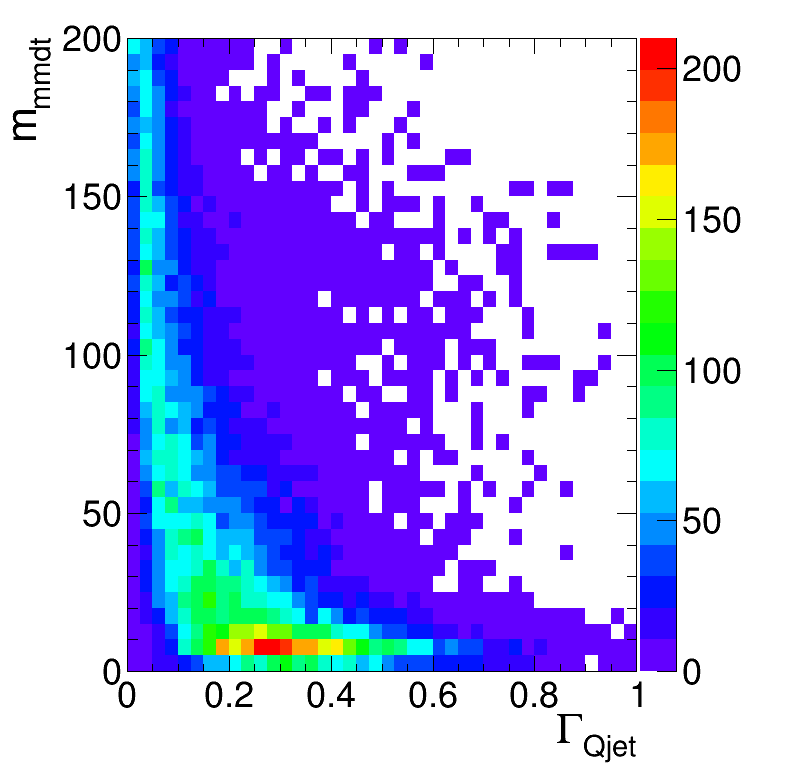
\includegraphics[width=0.48\textwidth]{./Figures/figs072514/figs071614_Wg_bin500_ak08/twoD/h2d_j_qjetVol_j_mass_mmdt_gg.png}}
\subfigure[mMDT mass vs $\tau_{21}^{\beta=1}$]{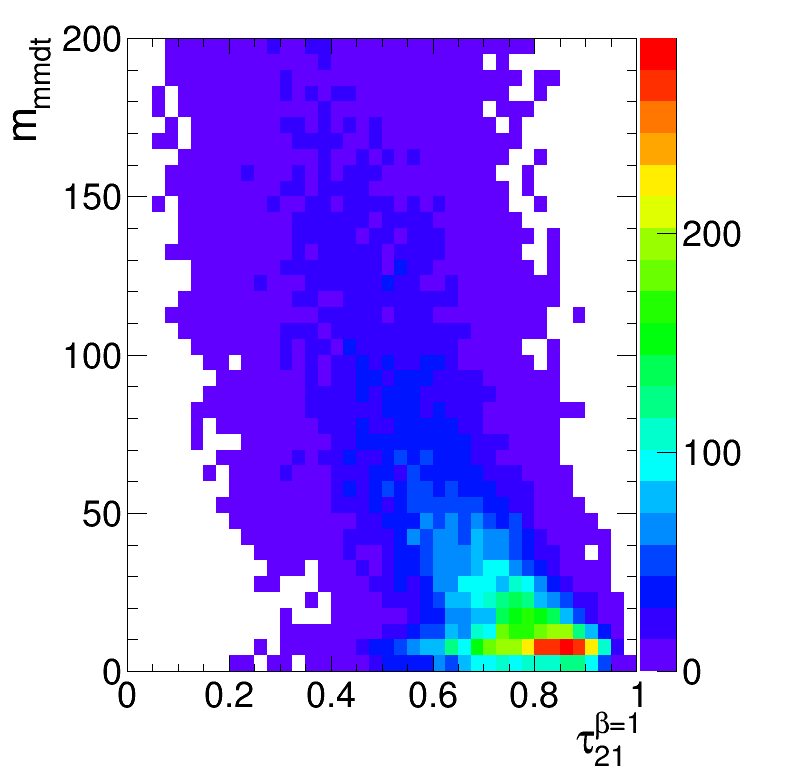
\includegraphics[width=0.48\textwidth]{./Figures/figs072514/figs071614_Wg_bin500_ak08/twoD/h2d_jtau21_b1_j_mass_mmdt_gg.png}}
\caption{2-D plots showing the correlation between mMDT mass and
  various substructure variables in the \pt 500 GeV bin using the
  anti-\kT R=0.8 algorithm in the gg sample.}
\label{fig:pt500_2d_mmdt_AKt_R08}
\end{center}
\end{figure*}

Figure~\ref{fig:pt500_2Dcomb_AKt_R12} shows the background efficiency
for a fixed signal efficiency (50\%) of each BDT combination of
each pair of variables considered, in the \pt 500 GeV bin, now using the anti-\kT R=1.2
algorithm. Compared to Figure~\ref{fig:pt500_2Dcomb_AKt_R08}, the
overall trends are similar, but there are clear differences in the
relative power of the mass + X combinations. Interestingly, the groomed masses are now all most improved by combination
with the $\tau_{21}^{\beta=1}$ variable, in contrast with
$C_{2}^{\beta=1}$ which performed best for the smaller radius of
R=0.8. 
%Q-jet volatility also performs markedly better than it did in
%the R=0.8 case. 
Figure~\ref{fig:pt500_masscomb_AKt_R12} shows the actual ROC curves
for the BDT combinations of
the best performant groomed masses with every other
variable considered in the \pt 500 GeV bin using the anti-\kT R=1.2
algorithm. 
%Interestingly, the groomed masses are now all most improved by combination
%with the $\tau_{21}^{\beta=1}$ variable, in contrast with
%$C_{2}^{\beta=1}$ which performed best for the smaller radius of
%R=0.8. 
One can see from Figure~\ref{fig:pt500_single_AKt_R12} that the
single variable discrimination of $\tau_{21}^{\beta=1}$ and
$C_{2}^{\beta=1}$ changes quite markedly when the distance parameter R
is varied, although in both cases $C_{2}^{\beta=1}$ is a better single
variable discriminant (except for very high signal
efficiencies). Figure~\ref{fig:pt500_subst_AKt_R08_R12} shows how the
actual distributions of the $C_{2}^{\beta=1}$ and $\tau_{21}^{\beta=1}$
change when we change the distance parameter. Figure~\ref{fig:pt500_2d_mmdt_AKt_R12} shows the 2-D
correlation plots between between the mMDT mass and the $C_{2}^{\beta=1}$,
$\Gamma_{Qjet}$ and $\tau_{21}^{\beta=1}$ variables for the R=1.2
case. It is hard to see a substantial difference in the correlations
here versus Figure~\ref{fig:pt500_2d_mmdt_AKt_R08}, but perhaps
$C_{2}^{\beta=1}$ is marginally more correlated with the mass for
R=1.2 compared to R=0.8.
{\it Andrew to add his explanation of why discrimination power of C2 versus tau21
  gets worse when we go to larger jet radii (email 0606/2014)}


{\it Now show a plot which compares on one plot the best combined performance for
each groomed mass + X for both R=0.8 and 1.2 cases e.g. mass +
$C_{2}^{\beta=1}$ for R=0.8 and mass + $\tau_{21}^{\beta=1}$ for R=1.2,
  and draw on also the
all variables curve for both R=0.8,1.2. 
Then we can see if there is much dependence on choice of mass once you
combine with another variable, and compare directly the two distance parameters.
This plot is just for
one kinematic bin, we should make the same plot for others.}

{\it Repeat these studies for different R and different kinematic
bins. Finally make plots which compare best combined performance for
different R and kinematics.}

{\it Do we want to look at other combinations of variables which don't
involve mass? Practically I think we will always be making mass + X though.}


\begin{figure*}
\begin{center}
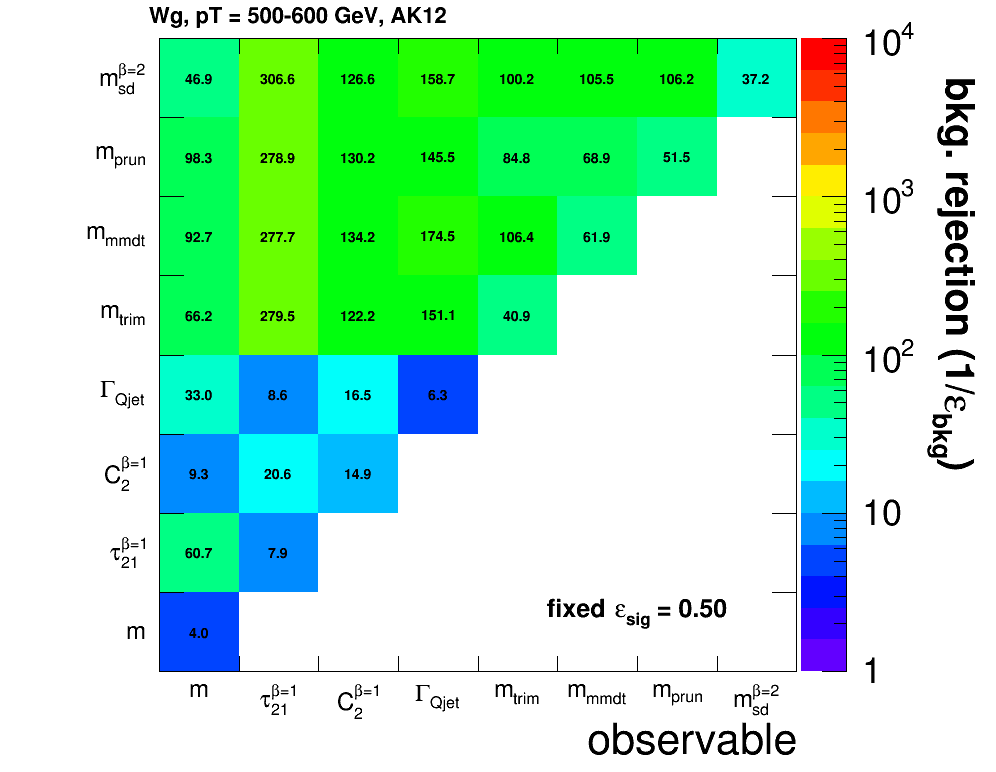
\includegraphics[width=0.48\textwidth]{./Figures/figs072514/figs071614_Wg_bin500_ak12/rocs/effBkg2D.png}
\caption{The background efficiency
for a fixed signal efficiency (50\%) of each BDT combination of
each pair of variables considered, in the \pt 500 GeV bin using the anti-\kT R=1.2
algorithm.}
\label{fig:pt500_2Dcomb_AKt_R12}
\end{center}
\end{figure*}

\begin{figure*}
\begin{center}
%\subfigure[Ungroomed mass + X]{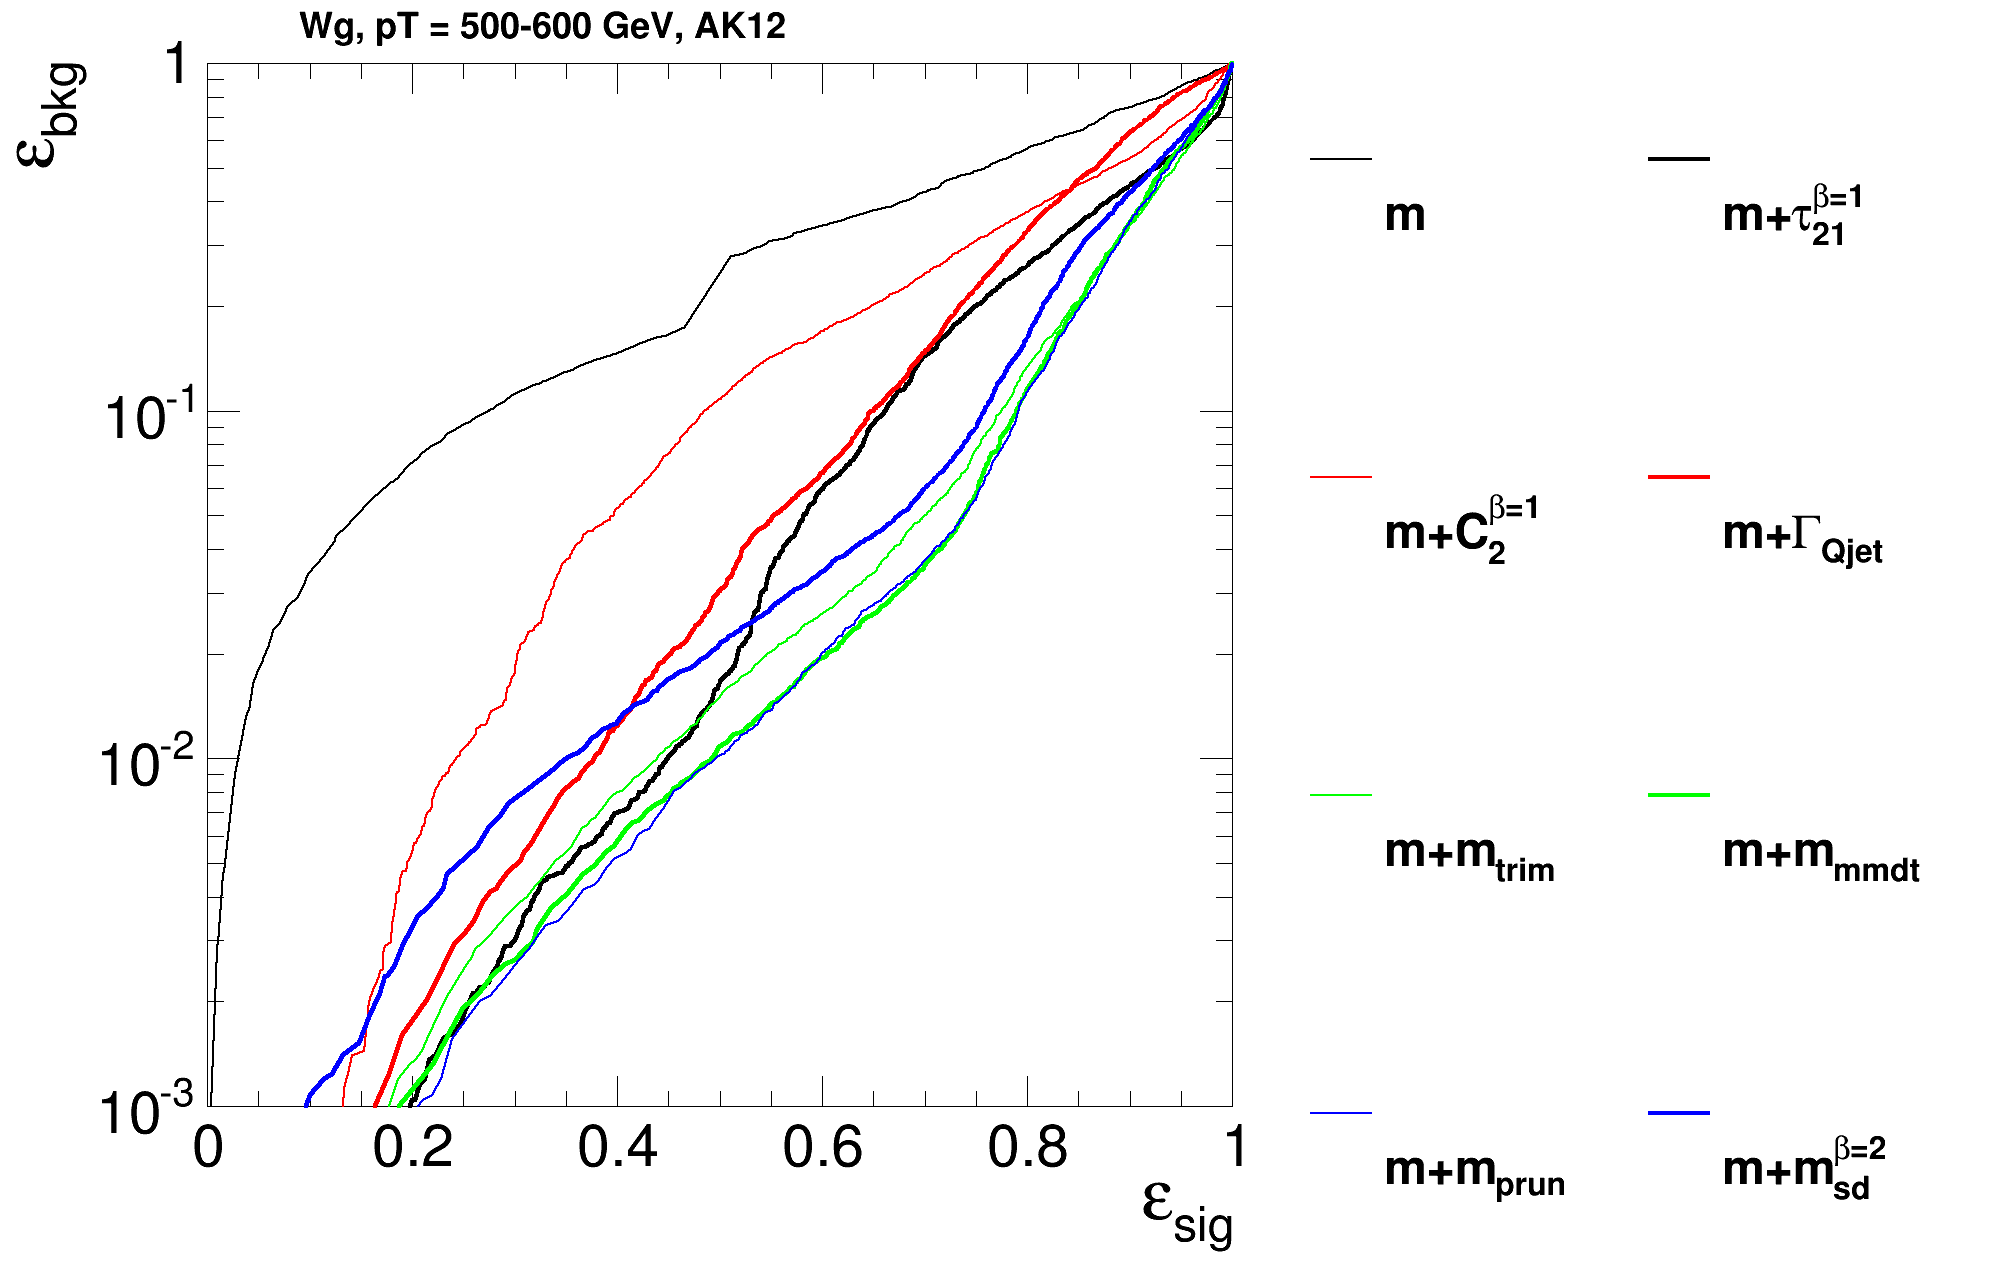
\includegraphics[width=0.48\textwidth]{./Figures/figs072514/figs071614_Wg_bin500_ak12/rocs/Rocs_1D_jmass.png}}
\subfigure[Trimmed mass + X]{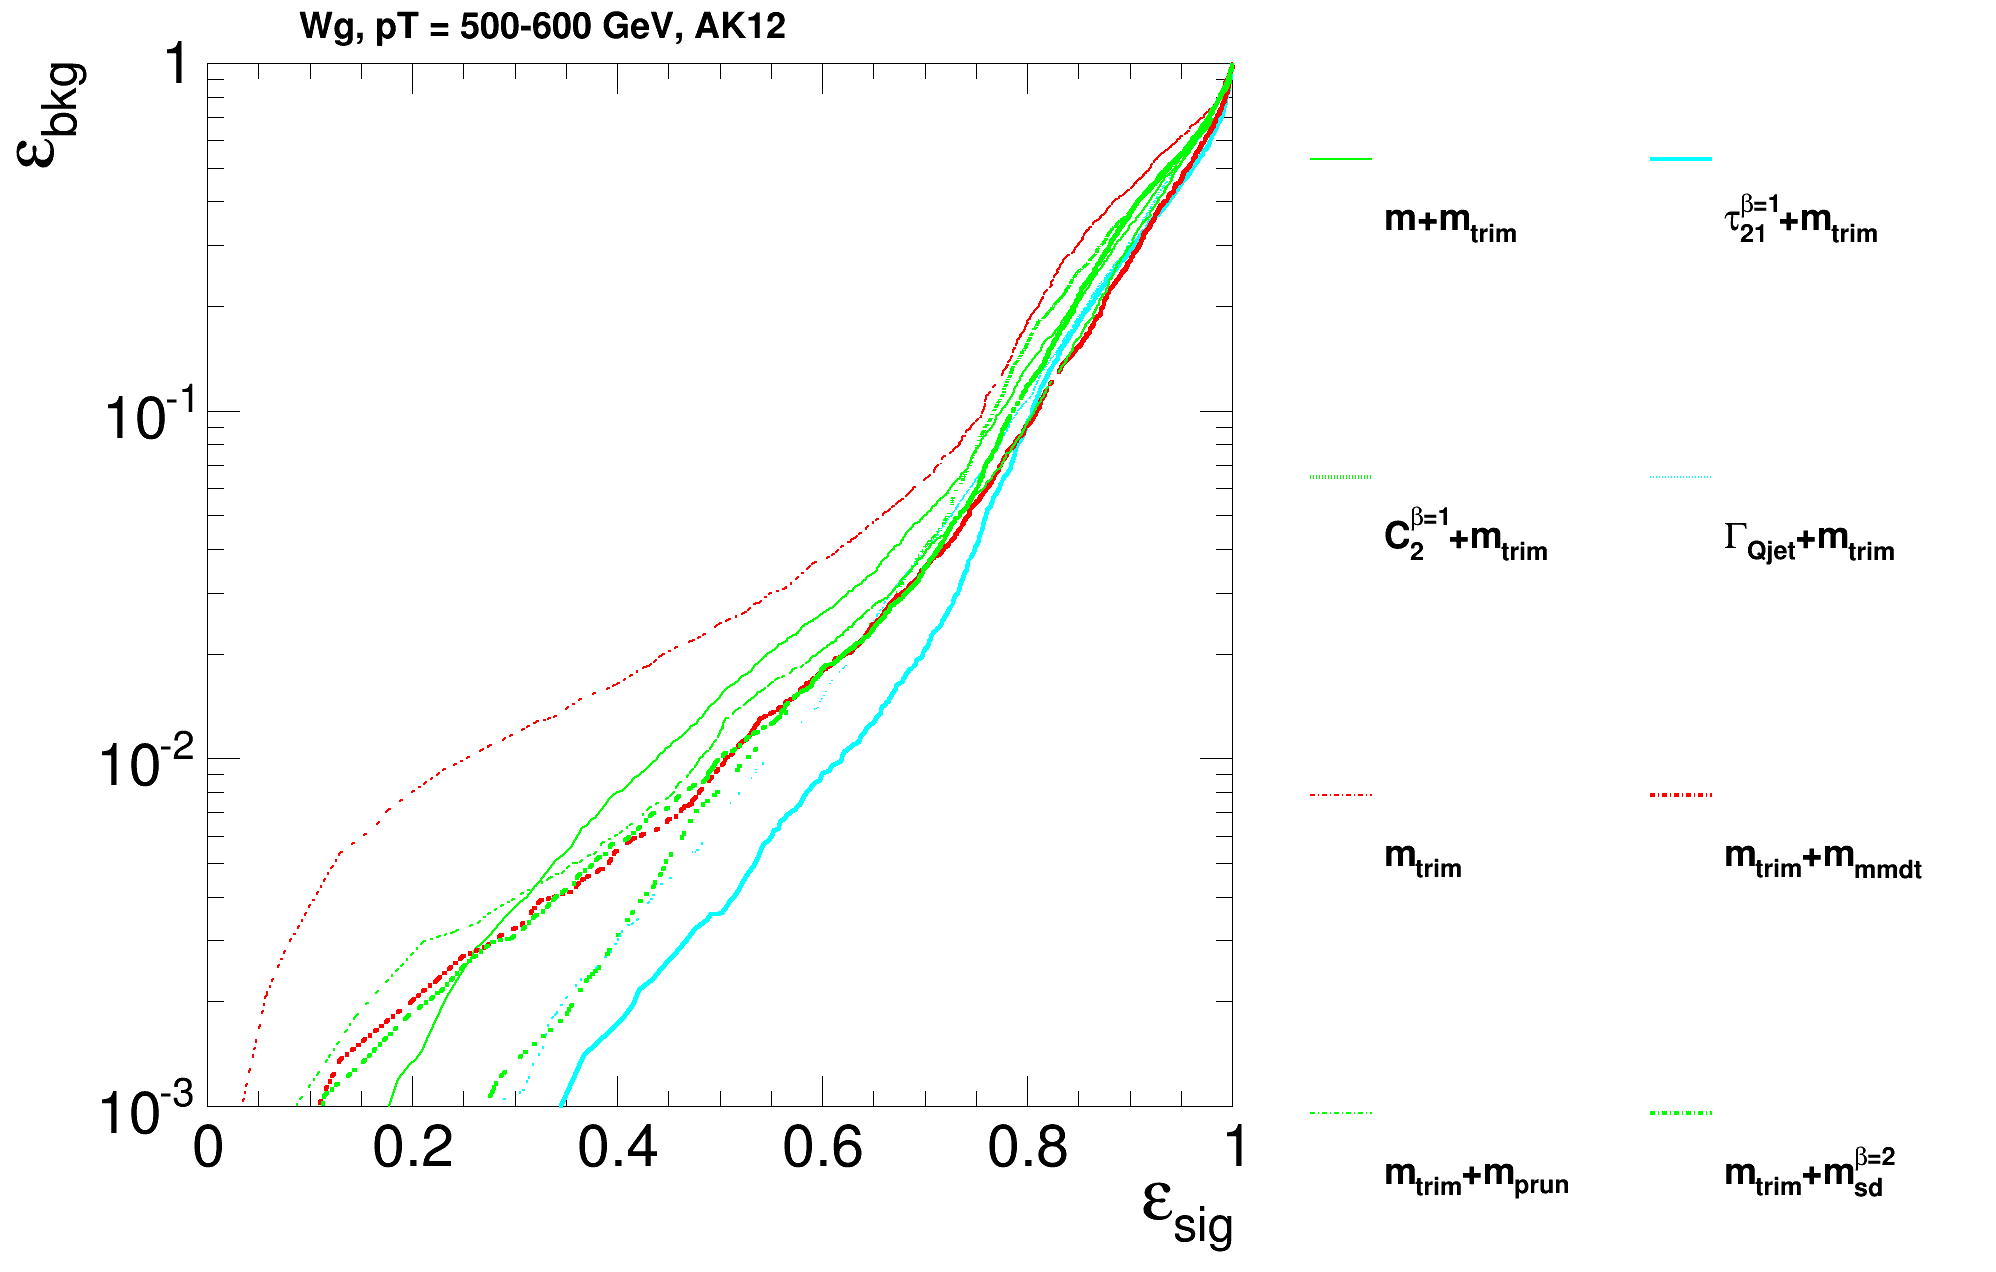
\includegraphics[width=0.48\textwidth]{./Figures/figs072514/figs071614_Wg_bin500_ak12/rocs/Rocs_1D_j_mass_trim.png}}
\subfigure[Pruned mass + X]{\includegraphics[width=0.48\textwidth]{./Figures/figs072514/figs071614_Wg_bin500_ak12/rocs/Rocs_1D_j_mass_prun.png}}
%\subfigure[Soft drop mass ($\beta=-1$) +X]{\includegraphics[width=0.48\textwidth]{./Figures/figs072514/figs071614_Wg_bin500_ak12/rocs/Rocs_1D_j_mass_sdm1.png}}
\subfigure[Soft drop mass ($\beta=2$) + X]{\includegraphics[width=0.48\textwidth]{./Figures/figs072514/figs071614_Wg_bin500_ak12/rocs/Rocs_1D_j_mass_sdb2.png}}
\subfigure[mMDT mass + X]{\includegraphics[width=0.48\textwidth]{./Figures/figs072514/figs071614_Wg_bin500_ak12/rocs/Rocs_1D_j_mass_mmdt.png}}
\caption{The BDT combinations of each mass variable with every other
variable considered in the \pt 500 GeV bin using the anti-\kT R=1.2 algorithm.}
\label{fig:pt500_masscomb_AKt_R12}
\end{center}
\end{figure*}

\begin{figure*}
\begin{center}
\subfigure[$C_2^{\beta=1}$, R=0.8]{\includegraphics[width=0.48\textwidth]{./Figures/figs072514/figs071614_Wg_bin500_ak08/oneD/h_c2_b1.png}}
\subfigure[$C_2^{\beta=1}$, R=1.2]{\includegraphics[width=0.48\textwidth]{./Figures/figs072514/figs071614_Wg_bin500_ak12/oneD/h_c2_b1.png}}
\subfigure[$\tau_{21}^{\beta=1}$, R=0.8]{\includegraphics[width=0.48\textwidth]{./Figures/figs072514/figs071614_Wg_bin500_ak08/oneD/h_tau21_b1.png}}
\subfigure[$\tau_{21}^{\beta=1}$, R=1.2]{\includegraphics[width=0.48\textwidth]{./Figures/figs072514/figs071614_Wg_bin500_ak12/oneD/h_tau21_b1.png}}
\caption{Comparisons of the QCD background to the WW signal in the \pt
  500 GeV bin for $C_2^{\beta=1}$ and $\tau_{21}^{\beta=1}$ variables
  and using the R=0.8 and R=1.2 anti-\kT distance parameters.}
\label{fig:pt500_subst_AKt_R08_R12}
\end{center}
\end{figure*}


\begin{figure*}
\begin{center}
\subfigure[mMDT mass vs $C_2^{\beta=1}$]{\includegraphics[width=0.48\textwidth]{./Figures/figs072514/figs071614_Wg_bin500_ak12/twoD/h2d_jc2_b1_j_mass_mmdt_gg.png}}
\subfigure[mMDT mass vs $\Gamma_{Qjet}$]{\includegraphics[width=0.48\textwidth]{./Figures/figs072514/figs071614_Wg_bin500_ak12/twoD/h2d_j_qjetVol_j_mass_mmdt_gg.png}}
\subfigure[mMDT mass vs $\tau_{21}^{\beta=1}$]{\includegraphics[width=0.48\textwidth]{./Figures/figs072514/figs071614_Wg_bin500_ak12/twoD/h2d_jtau21_b1_j_mass_mmdt_gg.png}}
\caption{2-D plots showing the correlation between mMDT mass and
  various substructure variables in the \pt 500 GeV bin using the
  anti-\kT R=1.2 algorithm in the gg sample.}
\label{fig:pt500_2d_mmdt_AKt_R12}
\end{center}
\end{figure*}


\subsubsection*{Mass + Mass Performance}
\label{sec:wtag_massplusmass}
It's interesting also to study and understand how the different
groomed masses relate to each other and how they are correlated.

Figures~\ref{fig:pt500_2d_massQQ_AKt_R08} and Figures~\ref{fig:pt500_2d_massGG_AKt_R08} shows 2-D correlation plots of
the different types of groomed mass in the \pt 500 GeV bin using the anti-\kT R=0.8
algorithm.

{\it Worth also showing some ROC curves for mass + mass combinations?}


\begin{table*}[htbp!]
\centering
%\setlength\fboxsep{0pt}
%\setlength\fboxrule{0.25pt}
\caption{Action of various groomers on the jet mass distribution in the different phase space regions.  For pruning, $a_\text{prune} = \zcut R_0$ and for trimming $a_\text{trim} = \sqrt{\zcut} R_\text{sub}$.}
\begin{tabular}{c|c|c|c|c} 
Action & Pruning & Trimming & mMDT & SD ($\beta > 0$) \\ \hline
$m>\sqrt{\zcut}R_0 p_T$  &  $-$ & $-$ &  $-$  & $-$ \\ \hline
\parbox[c][3em][c]{7em}{$m<\sqrt{\zcut}R_0 p_T$\\$m>a_x p_T$} & \parbox[c][3em][c]{6em}{cuts soft \& \\ soft-collinear}  & \parbox[c][3em][c]{6em}{cuts soft \& \\ soft-collinear} & \parbox[c][3em][c]{6em}{cuts soft \& \\ soft-collinear} & \parbox[c][5em][c]{7em}{cuts soft \& \\ partially ($\beta$) \\ on soft-collinear}  \\ \hline
$m<a_x p_T$ & \parbox[c][5em][c]{7em}{cuts partially \\ on both soft \& \\  soft-collinear}   &$-$ & \parbox[c][3em][c]{6em}{cuts soft \& \\ soft-collinear} & \parbox[c][5em][c]{7em}{cuts soft \& \\ partially ($\beta$) \\ on soft-collinear} 
\end{tabular}
\label{tab:boostedtoprates}
\end{table*}


\begin{figure*}
\begin{center}
\subfigure[Trimmed mass vs Soft drop mass ($\beta=2$)]{\includegraphics[width=0.48\textwidth]{./Figures/WTagging/pT500/AKtR08/WvsQ/h2d_j_mass_trim_j_mass_sdb2_WW_onSame.png}}
\subfigure[Trimmed mass vs Pruned mass]{\includegraphics[width=0.48\textwidth]{./Figures/WTagging/pT500/AKtR08/WvsQ/h2d_j_mass_trim_j_mass_prun_WW_onSame.png}}
\subfigure[Trimmed mass vs mMDT mass]{\includegraphics[width=0.48\textwidth]{./Figures/WTagging/pT500/AKtR08/WvsQ/h2d_j_mass_trim_j_mass_mmdt_WW_onSame.png}}
\subfigure[mMDT mass vs Soft drop mass ($\beta=2$)]{\includegraphics[width=0.48\textwidth]{./Figures/WTagging/pT500/AKtR08/WvsQ/h2d_j_mass_mmdt_j_mass_sdb2_WW_onSame.png}}
\subfigure[Pruned mass vs Soft drop mass ($\beta=2$)]{\includegraphics[width=0.48\textwidth]{./Figures/WTagging/pT500/AKtR08/WvsQ/h2d_j_mass_prun_j_mass_sdb2_WW_onSame.png}}
\subfigure[mMDT mass vs Pruned mass]{\includegraphics[width=0.48\textwidth]{./Figures/WTagging/pT500/AKtR08/WvsQ/h2d_j_mass_mmdt_j_mass_prun_WW_onSame.png}}
\caption{2-D plots showing the correlation between different types of
  groomed mass in the \pt 500 GeV bin using the anti-\kT R=0.8
  algorithm, separately for the jets in the $X \rightarrow WW$ sample and the
  jets in the quark-quark sample.}
\label{fig:pt500_2d_massQQ_AKt_R08}
\end{center}
\end{figure*}

\begin{figure*}
\begin{center}
\subfigure[Trimmed mass vs Soft drop mass ($\beta=2$)]{\includegraphics[width=0.48\textwidth]{./Figures/WTagging/pT500/AKtR08/WvsG/h2d_j_mass_trim_j_mass_sdb2_WW_onSame.png}}
\subfigure[Trimmed mass vs Pruned mass]{\includegraphics[width=0.48\textwidth]{./Figures/WTagging/pT500/AKtR08/WvsG/h2d_j_mass_trim_j_mass_prun_WW_onSame.png}}
\subfigure[Trimmed mass vs mMDT mass]{\includegraphics[width=0.48\textwidth]{./Figures/WTagging/pT500/AKtR08/WvsG/h2d_j_mass_trim_j_mass_mmdt_WW_onSame.png}}
\subfigure[mMDT mass vs Soft drop mass ($\beta=2$)]{\includegraphics[width=0.48\textwidth]{./Figures/WTagging/pT500/AKtR08/WvsG/h2d_j_mass_mmdt_j_mass_sdb2_WW_onSame.png}}
\subfigure[Pruned mass vs Soft drop mass ($\beta=2$)]{\includegraphics[width=0.48\textwidth]{./Figures/WTagging/pT500/AKtR08/WvsG/h2d_j_mass_prun_j_mass_sdb2_WW_onSame.png}}
\subfigure[mMDT mass vs Pruned mass]{\includegraphics[width=0.48\textwidth]{./Figures/WTagging/pT500/AKtR08/WvsG/h2d_j_mass_mmdt_j_mass_prun_WW_onSame.png}}
\caption{2-D plots showing the correlation between different types of
  groomed mass in the \pt 500 GeV bin using the anti-\kT R=0.8
  algorithm, separately for the jets in the $X \rightarrow WW$ sample and the
  jets in the gluon-gluon sample.}
\label{fig:pt500_2d_massGG_AKt_R08}
\end{center}
\end{figure*}


%\subsection{Performance at High Boosts}
%
%(this section is to cover the $W$-tagging performance for jet \pT 1-1.1 TeV and
%$>$ 1.5 TeV using $\sqrt{s} = 14$ TeV samples)
%
%{\it Maybe we don't need to divide into different medium/high boost sections.}




